%%==============================================================
%% Modelo de TCC para o curso de Sistemas de Informação
%% da Universidade Federal de Viçosa - Campus de Rio Paranaíba
%% Autor: Rodrigo Smarzaro (smarzaro@ufv.br)
%% Última versão Agosto/2021
%% Arquivo em formato UTF-8
%% Compilar com pdftex e biber
%% Precisa do arquivo abntex2-UFV.sty
%%==============================================================

\documentclass[
    % -- opções da classe memoir --
    12pt,                   % tamanho da fonte
    openright,              % capítulos começam em página ímpar (insere página vazia caso preciso)
    oneside,                % para impressão só no anverso. Oposto a twoside
    a4paper,                % tamanho do papel.
    % -- opções do pacote abntex2 --
    % chapter=TITLE,        % Títulos em maiúsculas
    sumario=tradicional,    % Sumário padrão memoir 
    % -- opções do pacote babel --
    english,                % idioma adicional para hifenização
    brazil,                 % idioma principal do documento
    ]{abntex2}

% Pacotes fundamentais
\usepackage{abntex2-UFV}        % Personalização para a Universidade Federal de Viçosa
\usepackage{lmodern}            % Usa a fonte Latin Modern
\usepackage[T1]{fontenc}        % Seleção de códigos de fonte de saída
\usepackage[utf8]{inputenc}        % Codificação do documento (conversão automática dos acentos)
\usepackage{indentfirst}        % Indenta o primeiro parágrafo de cada seção.
\usepackage{graphicx}            % Inclusão de gráficos
\usepackage{booktabs}           % \toprule, \midrule e \bottomrule para tabelas
\usepackage{csquotes}
\usepackage[final]{microtype} 			% para melhorias de justificação
\usepackage{hyphenat}

% Sistema autor-data com títulos nas referências em negrito
%\usepackage[alf,abnt-emphasize=bf]{abntex2cite}

% uso do biblatex, mais flexível e moderno
\usepackage[backend=biber,
            style=abnt,
            uniquename=init,
            giveninits,
            repeatfields,
            justify,
            noslsn]{biblatex}

\usepackage{xurl}

\urlstyle{same}

\addbibresource{referencias.bib}
%\bibliography{referencias}


%\PassOptionsToPackage{hyphens}{url}\usepackage{hyperref}
%\usepackage{url}
% permitir quebra de linha em URLs
%\makeatletter
%\g@addto@macro{\UrlBreaks}{\UrlOrds}
%\makeatother

%\setlength\bibparsep{10pt}

% ---
% CONFIGURAÇÕES DE PACOTES
% ---

% Informações de dados para CAPA e FOLHA DE ROSTO
\titulo{Desenvolvimento de um aplicativo mobile para otimização do transporte universitário intermunicipal de estudantes de São Gotardo - MG para a Universidade Federal de Viçosa - Campus de Rio Paranaíba}
\autor{Leandro Cesar Pereira}
\local{Rio Paranaíba}
\data{2023}
\orientador{Adriana Zanella Martinhago}    % redefinido no abntex2-UFV para aceitar Instituição (default = UFV-CRP)
%\coorientador{Nome do Coorientador}
\instituicao{Universidade Federal de Viçosa}

\campus{\emph{Campus} Rio Paranaíba}      % pacote abntex2-UFV
\curso{Sistemas de Informação}               % pacote abntex2-UFV
\membrobancaA{Membro da Banca A}             % pacote abntex2-UFV default = UFV-CRP
\membrobancaB{Membro da Banca B}       % pacote abntex2-UFV default = UFV-CRP
\databanca{\today}                           % pacote abntex2-UFV

% O preambulo deve conter o tipo do trabalho, o objetivo,
% o nome da instituição e a área de concentração
\preambulo{Monografia apresentada à Universidade Federal de Viçosa, como parte das exigências para a a aprovação na disciplina Trabalho de Conclusão de Curso I}
% ---

% ---
% Configurações de aparência do PDF final

% informações para o arquivo pdf de saída
% Interessante alterar a cor dos links para preto(black)
% na versão final para imprimir
\makeatletter
\hypersetup{
        % metadados
        pdftitle={\@title},
        pdfauthor={\@author},
        pdfsubject={\imprimirpreambulo},
        pdfcreator={LaTeX with abnTeX2},
        colorlinks=true,   % false: links em frame; true: links coloridos
        linkcolor=black,   % cor dos links no documento
        citecolor=blue,    % cor dos links para a bibliografia
        filecolor=magenta, % cor dos links para arquivos
        urlcolor=blue,     % cor dos links para sites
        bookmarksdepth=4   % profundidade do sumário do PDF
}
\makeatother
% ---

\begin{document}
% Retira espaço extra obsoleto entre as frases.
\frenchspacing

% ----------------------------------------------------------
% ELEMENTOS PRÉ-TEXTUAIS
% ----------------------------------------------------------
\pretextual

% Capa
\imprimircapa

% Folha de rosto
\imprimirfolhaderosto
% ---

% Inserir folha de aprovação
%\imprimirfolhadeaprovacao

% Dedicatória
%\begin{dedicatoria}
%   \vspace*{\fill}
%   \centering
%   \noindent
%   \textit{Texto qualquer da dedicatória}
%   \vspace*{\fill}
%\end{dedicatoria}
% ---

% Agradecimentos
%\begin{agradecimentos}
%Insira o texto de agradecimentos aqui
%\end{agradecimentos}
% ---

% Epígrafe
%\begin{epigrafe}
%    \vspace*{\fill}
%    \begin{flushright}
%        \textit{``Word? nunca mais.''\\
%        (Qualquer usuário de \LaTeX)}
%    \end{flushright}
%\end{epigrafe}
% ---

% RESUMOS

% resumo em português
\begin{resumo}
     Este trabalho aborda o desafio logístico e financeiro do transporte universitário entre São Gotardo-MG e Rio Paranaíba-MG.Apresento uma proposta de desenvolvimento de um aplicativo \textit{mobile} para auxiliar na organização do transporte dos estudantes para a UFV-CRP em Rio Paranaíba. O objetivo do aplicativo é oferecer uma solução tecnológica eficiente para resolver problemas como a falta de informações atualizadas sobre as rotas e pontos de parada, além da superlotação dos veículos e a falta de organização. O aplicativo irá fornecer funcionalidades como consulta de horários de transporte, acompanhamento em tempo real dos veículos e comunicação direta com os responsáveis pelo transporte. A metodologia adotada compreende etapas como o levantamento e especificação de requisitos, definição da arquitetura do aplicativo, desenvolvimento, validação e implantação. A eficácia do aplicativo será avaliada por meio de testes funcionais, testes de usabilidade e coleta de \textit{feedback} dos usuários. Espera-se que este trabalho contribua para a melhoria do transporte dos estudantes de São Gotardo até a UFV-CRP, proporcionando uma experiência mais organizada, eficiente e confortável.

    \vspace{\onelineskip}
    
    \noindent\textbf{Palavras-chave:} aplicativo \textit{mobile}, aplicativo de transporte, transporte universitário, transporte intermunicipal, melhoria da experiência acadêmica.

\end{resumo}

% resumo em inglês
\begin{resumo}[Abstract]
\begin{otherlanguage*}{english}
   This work addresses the logistical and financial challenges of university transportation between São Gotardo-MG and Rio Paranaíba-MG. I present a proposal for developing a mobile application to assist in organizing student transportation to UFV-CRP in Rio Paranaíba. The aim of the application is to offer an efficient technological solution to problems such as the lack of up-to-date information on routes and stops, as well as vehicle overcrowding and disorganization. The application will provide functionalities such as transport schedule consultation, real-time vehicle tracking, and direct communication with transportation coordinators. The adopted methodology includes steps such as requirement gathering, app architecture definition, development, validation, and deployment. The effectiveness of the application will be evaluated through functional tests, usability tests, and user feedback collection. It is expected that this work will contribute to improving student transportation from São Gotardo to UFV-CRP, providing a more organized, efficient, and comfortable experience.
    
    \vspace{\onelineskip}
    
    \noindent\textbf{Keywords:} mobile application, transport app, university transportation, intermunicipal transport, academic experience enhancement.
 \end{otherlanguage*}
\end{resumo}

% inserir lista de ilustrações
\pdfbookmark[0]{\listfigurename}{lof}
\listoffigures*
\cleardoublepage
% ---

% inserir lista de tabelas
%\pdfbookmark[0]{\listtablename}{lot}
%\listoftables*
%\cleardoublepage
% ---

% Lista de siglas e abreviaturas (opcional)
% sintaxe: \item [sigla] Descrição da sigla

\begin{siglas}
    \item[AESGUFVCRP] Associação dos Estudantes de São Gotardo na Universidade Federal de Viçosa \emph{Campus} Rio Paranaíba
    \item[API] \textit{Application Program Interface}
    \item[CRP] \emph{Campus} Rio Paranaíba
    \item[HTTP] \textit{Hypertext Transfer Protocol}
    \item[iOS] \textit{iPhone Operational System}
    \item[SGBD]Sistemas de Gerenciamento de Banco de Dados
    \item[UFV] Universidade Federal de Viçosa
    
    
\end{siglas}

% Lista de símbolos (opcional)
% sintaxe: \item [simbolo] Descrição do símbolo

%\begin{simbolos}
%\item[$\infty$ ] Infinito
%\end{simbolos}

% inserir o sumario
\pdfbookmark[0]{\contentsname}{toc}
\tableofcontents*
\cleardoublepage
% ---

% ----------------------------------------------------------
% ELEMENTOS TEXTUAIS
% ----------------------------------------------------------
\textual

%Modifique a estrutura dos capítulos e seções de acordo com a necessidade do seu trabalho
\chapter{Introdução}\label{sec:introducao}
     
    O transporte universitário é uma questão crucial para estudantes que precisam se deslocar diariamente entre cidades em busca de educação de qualidade. Essa realidade também se aplica às cidades de São Gotardo-MG e Rio Paranaíba-MG, onde as opções de transporte são limitadas e nem sempre são adequadas e acessíveis, podendo comprometer a frequência e o desempenho dos alunos.O transporte diário desses estudantes é essencial para garantir o acesso à universidade, mas muitas vezes enfrenta desafios como a falta de informações atualizadas, a e lotação dos veículos e a falta de organização.

    Esses estudantes enfrentam desafios logísticos e financeiros ao buscarem meios de transporte para chegar às instituições de ensino. A ausência de um serviço de transporte eficiente e de baixo custo afeta negativamente a experiência acadêmica, levando a dificuldades como cansaço excessivo, menos tempo para estudos, e desistência dos cursos \cite{Souza2016}.
    
    Diante dessa realidade é necessário buscar soluções que otimizem o transporte universitário entre essas cidades. Este trabalho irá analisar os desafios enfrentados pelos estudantes e propor uma alternativa de melhoria viável para melhorar a qualidade deste serviço, ao identificar e abordar essas questões, espera-se contribuir para a construção de um sistema de transporte universitário eficiente com a disponibilidade de forma mais acessível e organizadas dos dados do serviço no aplicativo \textit{móvel}, que atenda às necessidades dos estudantes melhore sua experiência acadêmico com um trasporte organizado e prático com o uso do aplicativo tendo acesso aos recursos do serviço pelo \textit{smartfone} \cite{freitas2020transporte}.
    
    E isto será feito neste trabalho aonde será desenvolvido de um aplicativo \textit{mobile} para auxiliar na organização do transporte dos estudantes de São Gotardo até a UFV-CRP em Rio Paranaíba.
    
    O restante deste trabalho está organizado da seguinte forma. Na Seção 2, descreve-se a base teórica para o desenvolvimento do aplicativo. Na Seção 3, são apresentados os Trabalhos Relacionados a este assunto. Na Seção 4, discutem-se os resultados esperados e quais seus impactos possíveis e melhorias proporcionadas. Por fim, na Seção 5, são apresentadas as conclusões.

    \section{Objetivos}\label{sec:objetivos}
        \label{sec:Objetivos}
        \subsection{Objetivo Geral}\label{sec:ObjetivosEspec}
            Desenvolver um aplicativo \textit{mobile} que ajude a organizar o transporte dos estudantes de São Gotardo até a UFV-CRP em Rio Paranaíba.
    
        \subsection{Objetivos Específicos}\label{sec:ObjetivosEspec}
            \begin{enumerate}
                \item Realizar um levantamento das principais necessidades dos estudantes em relação ao transporte até a UFV-CRP em Rio Paranaíba.
                \item Desenvolver um protótipo do aplicativo, com foco nas funcionalidades de cadastro de usuários, registro de rotas e disponibilidade de vagas no transporte.
                \item Implementar um sistema de geolocalização no aplicativo para auxiliar na identificação do ponto de encontro e na otimização das rotas.
                \item Realizar testes e validações do aplicativo em ambiente controlado, com participação dos estudantes de São Gotardo.
            \end{enumerate}


\chapter{Referencial Teórico}\label{sec:RefTeorico}

Neste capítulo, será apresentado o referencial teórico que fundamenta o desenvolvimento do trabalho. Serão discutidos conceitos e teorias relacionadas ao transporte universitário, aplicativos móveis e tecnologias utilizadas na construção do aplicativo. 

\section{Transporte Universitário}
\label{sec:transporte-universitario}

O transporte universitário é um serviço que visa facilitar o deslocamento dos estudantes entre suas residências e o \textit{Campus} da universidade. Ele é especialmente importante em regiões onde a universidade está distante e geralmente é feito em diferentes contextos como o transporte municipal e o intermunicipal.

     O transporte municipal refere-se ao serviço de transporte público disponibilizado pela prefeitura ou órgãos responsáveis pelo transporte na cidade onde a universidade está localizada, além de ter trasportes privados que oferecem este serviço aos estudantes também. Esse serviço tem como objetivo principal atender às necessidades de deslocamento dos estudantes universitários dentro do perímetro urbano, facilitando o acesso às instituições de ensino.
    
    O transporte municipal universitário desempenha um papel fundamental na mobilidade dos estudantes, proporcionando uma opção acessível e conveniente de deslocamento para a universidade. Esses serviços geralmente operam em horários específicos, alinhados com os horários de aulas e atividades acadêmicas, e possuem rotas que abrangem os principais pontos de embarque e desembarque frequentados pelos estudantes \cite{miranda2019infraestrutura}.

    
     O transporte intermunicipal refere-se ao serviço de transporte público ou privado entre diferentes municípios, especialmente quando há uma distância considerável entre a cidade de origem do estudante e a cidade onde a universidade está localizada. Esse tipo de transporte é projetado para atender às necessidades de estudantes que precisam viajar de uma cidade para outra para frequentar a universidade. Geralmente, o transporte intermunicipal universitário é fornecido por meio de ônibus ou vans, e possui horários e rotas específicas para atender à demanda dos estudantes. Esse serviço permite que os estudantes se desloquem de suas cidades de origem para a universidade de forma mais segura, confortável e eficiente.
    
    O transporte intermunicipal universitário desempenha um papel crucial na conectividade entre diferentes regiões e na promoção do acesso à educação superior para estudantes de localidades distantes. Além disso, existem os desafios enfrentados pelos estudantes que dependem do transporte intermunicipal para acessar a universidade, como a falta de horários adequados e a lotação dos veículos, uma referência para este contexto pode ser visto no trabalho na seção \cite{Souza2016}.
    
    Este trabalho está inserido em um contexto específico, pois se trata de um serviço de transporte intermunicipal entre as cidades de São Gotardo-MG e Rio Paranaíba-MG, realizado por meio de ônibus operados pela Associação dos Estudantes de São Gotardo na Universidade Federal de Viçosa - \textit{Campus} Rio Paranaíba (AESGUFVCRP). Embora seja um serviço de transporte privado, a AESGUFVCRP recebe auxílio da Prefeitura de São Gotardo-MG para redução dos valores das passagens. No entanto, é importante ressaltar que esse apoio financeiro fornecido pela prefeitura não é garantido e varia em termos de valor.

\section{Dispositivos Móveis}
\label{sec:dispositivos-moveis}

Os dispositivos móveis revolucionaram a forma como nos comunicamos e interagimos com o mundo digital. Inicialmente, os telefones celulares foram desenvolvidos com o propósito principal de comunicação sem fio, permitindo que as pessoas se conectassem em qualquer lugar. Com o passar do tempo, esses dispositivos foram evoluindo, incorporando recursos cada vez mais avançados \cite{adrenaline-evolucao-celulares}.

O surgimento dos \textit{smartphones} foi um marco significativo na história dos dispositivos móveis. Esses dispositivos combinam a funcionalidade de um telefone celular com a capacidade de executar uma ampla variedade de aplicativos e acessar à Internet. Os \textit{smartphones} modernos oferecem telas sensíveis ao toque, permitindo interações intuitivas e uma experiência de usuário aprimorada\cite{adrenaline-evolucao-celulares}.

Além disso, os dispositivos móveis estão equipados com vários sensores integrados, como acelerômetro, giroscópio, GPS e sensor de luz. Esses sensores permitem que os aplicativos móveis obtenham informações sobre a localização do dispositivo, detectem movimentos e ajustem automaticamente a interface do usuário com base nas condições ambientais \cite{techtudo-smartphone}.

A conectividade de rede é outra característica fundamental dos dispositivos móveis. Com acesso à Internet os usuários podem se comunicar, acessar informações, fazer transações financeiras e usar uma ampla gama de serviços \textit{online}. A rápida evolução das redes móveis, como 3G, 4G e agora 5G, oferece velocidades de conexão cada vez mais rápidas e de maior capacidade.

Por fim, o poder de processamento dos dispositivos móveis tem aumentado consideravelmente. Os avanços na tecnologia de processadores e a otimização dos sistemas operacionais permitem que os dispositivos móveis executem aplicativos complexos e exigentes em termos de recursos. Isso possibilita o desenvolvimento de aplicativos móveis sofisticados, como os aplicativos de transporte universitário, que oferecem recursos de geolocalização, planejamento de rotas e interações em tempo real.

Para os funcionamento e operação dos dispositivos móveis são essenciais diversos recursos e o gerenciamento destes recursos fica por responsabilidade do sistema operacional, sendo importante e extremante relevante para o processo de desenvolvimento.

\subsection{Sistemas Operacionais}
\label{subsec:sistemas-operacionais}

Existem diversos sistemas operacionais móveis como Android, iOS, \textit{KaiOS}, \textit{Windows Phone}. Porém, os dois principais são o Android e o iOS que juntos representam mais de 99\% do mercado \cite{statcounter}, eles são os principais ambientes nos quais os aplicativos móveis são executados atualmente. Esses sistemas operacionais são desenvolvidos por diferentes empresas e possuem características distintas que influenciam a experiência do usuário e a compatibilidade dos aplicativos.

\subsection{Android}
\label{subsubsec:android}

O Android, desenvolvido pela empresa Google, é um sistema operacional amplamente utilizado em dispositivos móveis em todo o mundo. Ele se destaca por ser um sistema de código aberto, o que significa que pode ser personalizado e adaptado por fabricantes de dispositivos e desenvolvedores independentes \cite{android}. 
O Android oferece suporte a uma ampla variedade de dispositivos e possui uma grande base de usuários, tanto globalmente quanto no Brasil \cite{statcounter}. 

\subsection{iOS}
\label{subsubsec:ios}

O iOS, desenvolvido pela empresa Apple, é um sistema operacional exclusivo para dispositivos móveis da Apple, como iPhones e iPads. O iOS se destaca por sua integração vertical entre hardware e software, proporcionando uma experiência coesa e otimizada. Embora o iOS tenha uma participação de mercado menor em relação ao Android globalmente, ele é bastante popular entre os usuários de dispositivos móveis no Brasil \cite{statcounter-br}.

Os sistemas operacionais Android e iOS dominam o mercado de dispositivos móveis, e considerar suas diferenças e características distintas é essencial para o desenvolvimento de aplicativos móveis de sucesso.


\section{Aplicativos Móveis}
\label{sec:aplicativos-moveis}
Os aplicativos móveis são programas desenvolvidos para serem executados em dispositivos móveis, como \textit{ smartphones} e \textit{tablets}. Eles são projetados para aproveitar os recursos e as funcionalidades desses dispositivos, oferecendo uma ampla gama de serviços e utilidades para os usuários.

Esses aplicativos são desenvolvidos com o objetivo de proporcionar uma experiência interativa e personalizada, aproveitando recursos como telas sensíveis ao toque, câmeras, sensores, conectividade de rede e poder de processamento dos dispositivos móveis. Eles oferecem uma ampla variedade de funcionalidades, desde jogos e entretenimento até serviços de produtividade, redes sociais, educação, saúde, transporte e muito mais \cite{aplicativosmoveis}.

Os aplicativos móveis desempenham um papel significativo em nossa vida cotidiana, facilitando tarefas, fornecendo informações em tempo real, permitindo a comunicação instantânea e oferecendo acesso à serviços e conteúdos de forma conveniente. Eles se tornaram uma parte essencial na forma como interagimos com o mundo digital, transformando a maneira como nos comunicamos, trabalhamos, aprendemos, nos divertimos e nos deslocamos \cite{aplicativosmoveis}.

Existem diferentes tipos de aplicativos móveis, cada um com suas características e abordagens de desenvolvimento. Os aplicativos nativos são desenvolvidos especificamente para uma plataforma, como Android ou iOS, e podem tirar total proveito dos recursos do dispositivo. Os aplicativos web são acessados por meio de um navegador da web no dispositivo móvel e podem ser desenvolvidos usando tecnologias web padrão. Já os aplicativos híbridos combinam elementos de aplicativos nativos e aplicativos web, oferecendo uma abordagem mais flexível para o desenvolvimento em várias plataformas, cada um com seus pontos de diferenciação \cite{accurate-nativexmult}.

A escolha entre esses tipos de aplicativos móveis depende das necessidades do projeto, do público-alvo e dos recursos disponíveis. Cada abordagem tem suas vantagens e desvantagens, e é importante avaliar cuidadosamente as opções antes de iniciar o desenvolvimento de um aplicativo móvel, poderá ser visto de forma mais detalhada sobre o que são Aplicativos Nativos na seção \ref{subsec:aplicativos-nativos} e Aplicativos Híbridos na seção \ref{subsec:aplicativos-multiplataforma}.

Conforme o trabalho \cite{pinheiro-analise-apps-mobile} que faz uma análise completa das diferenças de desenvolvimento de aplicativos em linguagens nativas dos sistemas e aplicativos móveis multiplataforma, e demonstrado o tamanho impacto destas tecnologias, e as vantagens e desvantagens dos métodos, que fundamentam os argumentos apresentados nesta seção, como os impactos em desempenho e dificuldades de implementação de algum recurso.

A Figura \ref{fig:nativevsmultplataform} ilustra de forma simplificada a comparação entre as tecnologias de desenvolvimento mencionadas, onde é demonstrado que aplicações web app tem extremas desvantagem porém as tecnologias de apps nativos e híbridos tem diferenças bem menores umas em relação às outras, sendo as mais plausíveis para o desenvolvimento, por terem desempenho e segurança semelhante, porem com diferenças pequenas em áreas como usabilidade e UX/UI onde os apps nativos tem desvantagem.

\begin{figure}[!h]
  \begin{center}
  \centering
  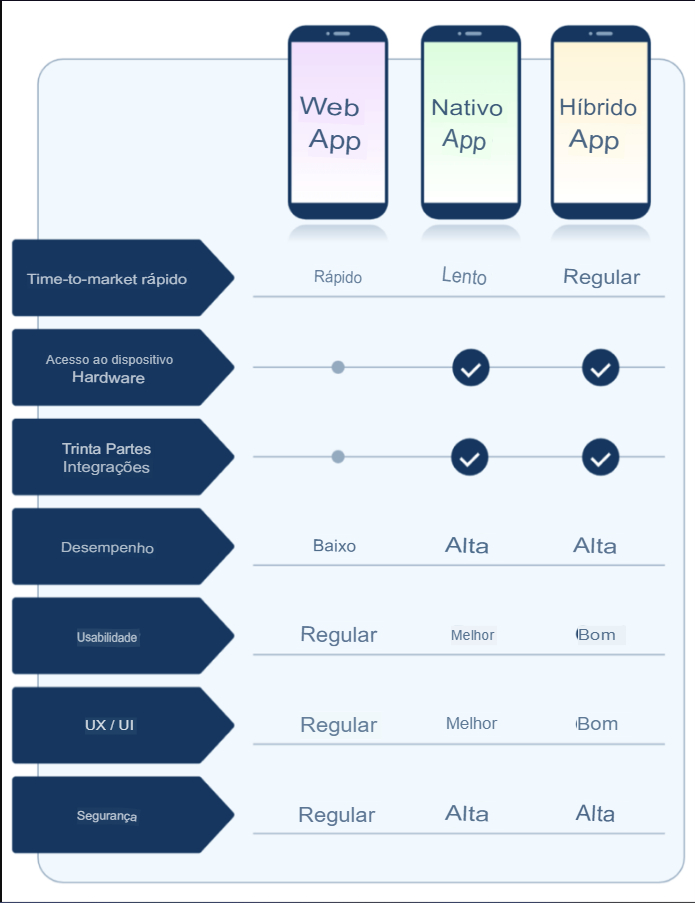
\includegraphics[width=0.8\linewidth]{Imagens/NativevsMulplataforma.png}
  \end{center}
  \caption[Comparação entre Tecnologias de Desenvolvimento]{Comparação Entre Tecnologias Nativas e Multiplataforma de Desenvolvimento Mobile}
  \label{fig:nativevsmultplataform}
  \legend{Fonte: \cite{infraestruturaaplicativo}}
\end{figure}

\newpage

No contexto do transporte universitário, os aplicativos móveis desempenham um papel importante na melhoria da experiência dos estudantes e na otimização da gestão do serviço. Eles oferecem recursos como visualização de rotas, horários, compra de passagens e comunicação direta com os usuários.

\subsection{Aplicativos em Linguagens Nativas dos Sistemas}
\label{subsec:aplicativos-nativos}
Os aplicativos móveis podem ser desenvolvidos utilizando as linguagens de programação nativas de cada sistema operacional, como Java ou Kotlin para Android e Objective-C ou Swift para iOS. Essa estratégia permite explorar todas as funcionalidades e recursos específicos de cada plataforma de forma direta e otimizada \cite{pinheiro-analise-apps-mobile}. No entanto, é importante considerar as vantagens e desvantagens.

\textbf{Vantagens}
\begin{itemize}
  \item \textbf{Desempenho}: Os aplicativos desenvolvidos em linguagens nativas geralmente apresentam melhor desempenho, pois podem aproveitar totalmente os recursos do dispositivo e as otimizações do sistema operacional.
  \item \textbf{Acesso completo às APIs}: O desenvolvimento nativo permite o acesso completo às APIs e bibliotecas específicas de cada plataforma, possibilitando a criação de recursos avançados e integrações profundas com o sistema.
\end{itemize}

\textbf{Desvantagens}
\begin{itemize}
  \item \textbf{Custo e tempo de desenvolvimento}: Desenvolver um aplicativo nativo para cada plataforma requer conhecimento específico das linguagens e  \textit{frameworks} utilizados, o que pode demandar mais tempo e recursos financeiros.
  \item \textbf{Manutenção}: Manter aplicativos nativos em diferentes plataformas pode ser complexo, pois qualquer atualização ou correção precisa ser implementada separadamente em cada versão do aplicativo.
\end{itemize}

\subsection{Aplicativos Móveis Multiplataforma}
\label{subsec:aplicativos-multiplataforma}
Outra forma de desenvolvimento de aplicativos é utilizando tecnologias multiplataforma, como React Native, Flutter ou Xamarin. Essas tecnologias permitem criar aplicativos que são executados em várias plataformas utilizando um único conjunto de código \cite{accurate-nativexmult}. Assim como na abordagem nativa, é importante considerar as vantagens e desvantagens dessa abordagem:

\textbf{Vantagens}
\begin{itemize}
  \item \textbf{Economia de tempo e recursos}: Com o desenvolvimento multiplataforma, é possível criar um único código-base que pode ser compartilhado entre diferentes plataformas, reduzindo o tempo e os custos de desenvolvimento.
  \item \textbf{Manutenção simplificada}: Atualizações e correções podem ser aplicadas de forma mais rápida e eficiente, pois são refletidas em todas as versões do aplicativo simultaneamente.
\end{itemize}

\textbf{Desvantagens}
\begin{itemize}
  \item \textbf{Desempenho}: Apesar das melhorias recentes, os aplicativos multiplataforma ainda podem apresentar um desempenho ligeiramente inferior em comparação aos aplicativos nativos, devido à camada adicional de abstração.
  \item \textbf{Limitações das APIs}: Nem todas as APIs e recursos específicos de cada plataforma podem ser acessados diretamente em aplicativos multiplataforma, o que pode restringir a implementação de certos recursos avançados.
\end{itemize}

Esta será a forma escolhida para o desenvolvimento da aplicação, pois não existe grande necessidades por desempenho, e nem uso de muitos recursos específicos de algum sistema, e as vantagens de economia de tempo e recursos e manutenção simplificada são pontos bem mais importantes para o contexto da aplicação.

\section{Tecnologias Utilizadas}
\label{sec:tecnologias-utilizadas}

Nesta seção serão descritas as tecnologias utilizadas no desenvolvimento do nosso sistema de gestão do transporte universitário.

\subsection{React Native}
\label{subsec:react-native}

O \textit{React Native} é um \textit{framework} de desenvolvimento de aplicativos móveis multiplataforma desenvolvido pela empresa Meta (antiga Facebook). Ele permite a criação de aplicativos nativos para Android e iOS usando uma única base de código escrita em \textit{JavaScript}. O \textit{React Native} utiliza componentes reutilizáveis, que são renderizados de forma nativa, proporcionando um desempenho e uma experiência de usuário semelhante aos aplicativos nativos tradicionais. Além disso, o \textit{React Native} possui uma grande comunidade de desenvolvedores e uma vasta biblioteca de componentes prontos para uso, acelerando o processo de desenvolvimento \cite{alura-react-native}.

Uma tecnologia focada em facilitar o desenvolvimento algo que pode ser visto em sua página oficial do aonde é demonstrado o foco em versatilidade no desenvolvimento de aplicativos mobile  \cite{reactnative}

 Essas vantagens tornam o \textit{React Native} uma escolha vantajosa para o desenvolvimento de aplicativos móveis, especialmente do ponto de vista do mercado atual.Isso pode ser visto em diversos artigos que abordam diretamente as vantagens da tecnologia \textit{React Native} para o desenvolvimento de aplicativos móveis \cite{alura-dev-apps-mobile}, \cite{alura-react-native}. 

A Figura \ref{fig:arquitetura-react-native} representa a arquitetura do \textit{React Native}, e demonstrado como esta tecnologia permite o desenvolvimento de aplicativos móveis nativos para iOS e Android usando \textit{JavaScript}. O \textit{React Native} combina a eficiência do desenvolvimento web com a experiência de usuário e o desempenho de aplicativos nativos. A arquitetura inclui o \textit{JavaScriptCore} como o motor \textit{JavaScript}. O \textit{Bridge} para comunicação entre \textit{JavaScript} e código nativo. O \textit{Framework Core} com bibliotecas nativas e a camada de interface do usuário onde os componentes visuais são criados usando JSX(\textit{JavaScript Syntax Extension}), sendo uma forma de criar elementos para serem utilizadas como \textit{templates} de aplicações React que facilita o desenvolvimento e aumenta o reaproveitamento do código. Essa abordagem simplifica o desenvolvimento multiplataforma e economiza tempo e esforço para criar aplicativos nativos separados para cada plataforma.

\begin{figure}[!h]
  \begin{center}
  \centering
  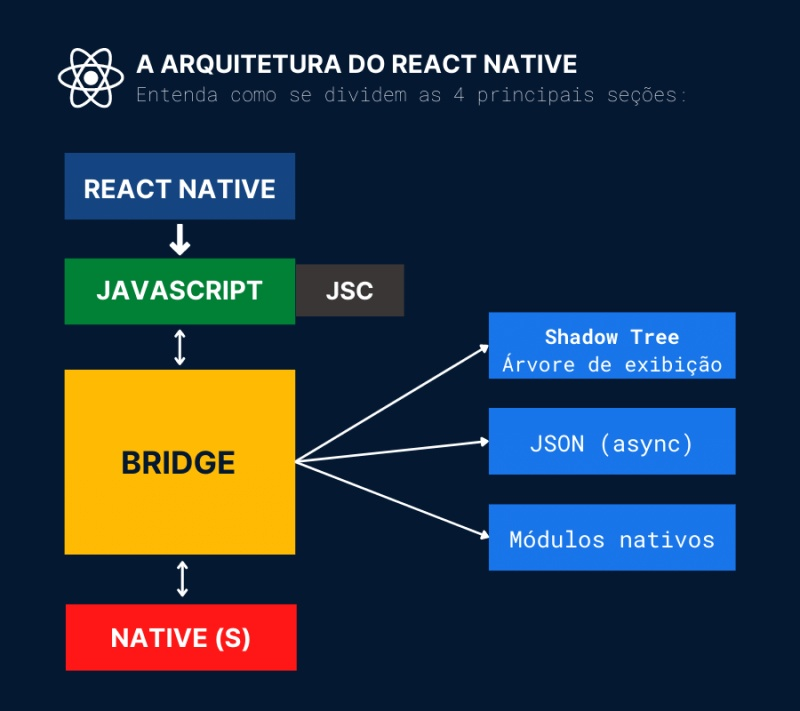
\includegraphics[width=1\linewidth]{Imagens/arquitetura-react-native.jpg}
  \end{center}
  \caption[Imagem da Arquitetura do React Native]{ 
  Demonstração da Arquitetura do React Native}
  \label{fig:arquitetura-react-native}
  \legend{Fonte: \cite{alura-react-native}}
\end{figure}

\newpage

\subsection{APIs de Geolocalização}
\label{subsec:apis-geolocalizacao}

Para a implementação de recursos de localização e rastreamento no aplicativo de transporte universitário será utilizado APIs de geolocalização. Essas APIs fornecem funcionalidades para obter a localização atual do dispositivo, calcular distâncias, traçar rotas e exibir mapas interativos. No caso do Android, será utilizado a API de Geolocalização do Google \cite{devmedia-google-maps}, que se integra perfeitamente com o sistema operacional. Já no iOS, também será usada a API de Geolocalização do Google \cite{devmedia-google-maps}. Essas APIs permitem a obtenção de dados precisos de localização em tempo real, essenciais para a funcionalidade de monitoramento e rastreamento do transporte universitário.

\subsection{Sistemas de Informação Geográfica}
\label{subsec:sistemas-informacao-geografica}

Os Sistemas de Informação Geográfica (SIG) são ferramentas utilizadas para capturar, armazenar, analisar e visualizar dados geográficos. Esses sistemas permitem que os operadores do transporte universitário gerenciem informações geográficas essenciais, como rotas, pontos de embarque e desembarque, áreas de cobertura e outros elementos relevantes para o serviço, o SIG será usando principalmente para a parte de visualização dos dados geográficos no aplicativo, porém por parte dos administradores do sistema será usado também para recolher e verificar os dados antes de incorporar ao banco de dados do serviço \cite{bolfe2018sistemas}.

Os SIG são capazes de criar e manipular mapas digitais que apresentam dados geográficos de forma interativa. Além disso, esses sistemas podem ser integrados aos aplicativos móveis, proporcionando aos usuários a possibilidade de acessar mapas interativos, pesquisar rotas, localizar pontos de embarque próximos e obter informações geográficas em tempo real. Essa integração com os aplicativos móveis amplia a experiência do usuário e fornece recursos de geolocalização e navegação que facilitam o uso do transporte universitário \cite{bolfe2018sistemas}.

Os SIG terão o papel importante no gerenciamento e visualização de informações geográficas no  trabalho, a visualização será feita a partir do uso das funções da biblioteca \textit{React Native Maps} \cite{logrocket-react-native-maps}, biblioteca \textit{JavaScript} que permitira a visualização dos dados em mapas interativos no aplicativo.

\subsection{Bancos de Dados}
\label{subsec:bancos-dados}

No contexto do desenvolvimento do sistema de gestão do transporte universitário, é importante empregar um banco de dados que possibilite a armazenagem e administração eficazes de informações cruciais. Além disso, a utilização de um Sistema de Gerenciamento de Banco de Dados (SGBD) é essencial para gerir esses bancos de dados, permitindo a manipulação de variados aspectos, como os registros dos usuários, rotas de ônibus, horários e outras informações pertinentes ao serviço.

Um banco de dados é um sistema de armazenamento e recuperação de informações estruturadas de forma organizada. Ele permite a criação, atualização, consulta e remoção de dados de maneira eficiente.

Um SGBD é um software responsável por gerenciar o armazenamento e a recuperação de dados em um banco de dados. Ele fornece uma interface para criar, manipular e consultar informações de forma eficiente e segura. Além disso, o SGBD gerencia aspectos como a integridade dos dados, a segurança, o controle de acesso e a otimização de consultas \cite{elmasri2000sistemas}.

Optou-se por utilizar o Sistema Gerenciador de Banco de Dados relacional MySQL, pois ele já está incorporado em sistemas existentes da AESGUFVCRP, facilitando assim sua implementação e utilização, também são consideráveis suas vantagens, como sua estabilidade, flexibilidade e ampla adoção na indústria \cite{mysql}. Além do MySQL oferece recursos avançados de consulta e manipulação de dados, garantindo um ambiente confiável para o armazenamento das informações do sistema de gestão do transporte universitário. Além disso, o MySQL conta com uma vasta documentação sendo suportado por uma comunidade ativa, o que facilita a resolução de dúvidas e problemas.

\subsection{\textit{Frameworks} Complementares}
\label{subsec:frameworks-complementares}

Além das tecnologias mencionadas anteriormente, serão utilizados alguns \textit{frameworks} complementares para auxiliar no desenvolvimento do sistema de gestão do transporte universitário. Entre eles, destaca-se o \textit{Axios} \cite{axios}, um cliente HTTP baseado em \textit{Promises} que são objetos que representa a eventual conclusão (ou falha) de uma operação assíncrona e seu valor resultante, que nos permite realizar requisições HTTP assíncronas para interagir com APIs externas, como o servidor de autenticação e o servidor de rotas do transporte universitário. Também será utilizado o \textit{Redux} \cite{redux}, um gerenciador de estado previsível para aplicações \textit{JavaScript}, que ajuda a centralizar e controlar o estado global do aplicativo, facilitando a comunicação entre os componentes.


\chapter{Trabalhos Relacionados}\label{sec:trabalhos-relacionado}

Nesta seção, são apresentados alguns trabalhos relacionados que abordam temas semelhantes ao trabalho proposto. 

\section{Automatização da Administração do Transporte Intermunicipal de Estudantes – Tupã/Marília}
\label{sec:TransporteIntermunicipalSouza2016}

\cite{Souza2016} descreve o desenvolvimento de um sistema de gestão do transporte intermunicipal universitário entre as cidades de Tupã e Marília. O objetivo principal do sistema é fornecer informações relevantes aos passageiros universitários, tais como a emissão de boletos de mensalidade, a quantidade de passageiros que utilizam o transporte, o valor da diária dos ônibus e a quantidade de ônibus contratados. Algumas dessas funcionalidades se assemelham às que estarão presentes na aplicação desenvolvida neste trabalho.

A plataforma proposta para o sistema é exclusivamente voltada para dispositivos Android e foi desenvolvida utilizando a linguagem de programação Java. Um ponto onde os trabalhos se diferem é a escolha de para quais sistemas a aplicação será desenvolvida, pois utilizando a tecnologia React Native será possível desenvolver para ambas neste trabalho. Essa abordagem permite alcançar um público mais amplo de usuários, abrangendo tanto os usuários de dispositivos Android quanto os de iOS.

Este trabalho relacionado é relevante para o trabalho proposto, uma vez que ambos abordam o desenvolvimento de aplicativos móveis para a gestão do transporte, embora apresentem diferenças na plataforma de desenvolvimento, bem como algumas funcionalidades específicas. A análise comparativa entre essas abordagens pode fornecer  \textit{insights} valiosos sobre as vantagens e desafios de cada uma delas, auxiliando na tomada de decisões e no aprimoramento do nosso próprio aplicativo. 


\section{UFRGS caronas: um aplicativo móvel de caronas para a comunidade da UFRGS}
\label{sec:caronasufrgsboranga2019}

\cite{boranga2019ufrgs} descreve o desenvolvimento de um aplicativo móvel de caronas para a comunidade da Universidade Federal do Rio Grande do Sul (UFRGS). O objetivo desse aplicativo é permitir que as pessoas compartilhem caronas e otimizem o deslocamento dentro do \textit{Campus} universitário. O aplicativo visa reduzir o tráfego, proporcionar mais conforto aos usuários de carona e promover a interação entre os membros da comunidade acadêmica.

É importante destacar que, em comparação com o trabalho \ref{sec:caronasufrgsboranga2019}, este trabalho tem uma abordagem mais ampla, desenvolvendo um aplicativo móvel para a gestão do transporte universitário em ambas as plataformas Android e iOS, utilizando a tecnologia React Native. Por outro lado, o trabalho \ref{sec:caronasufrgsboranga2019} foi desenvolvido apenas para a plataforma iOS usando linguagem nativa para apps do sistema e ferramentas da Apple. Essa abordagem diferente permite atingir um público mais amplo de usuários, abrangendo tanto os usuários de dispositivos Android quanto os de iOS.

A análise de tais trabalhos pode fornecer visões valiosos sobre as diferentes abordagens utilizadas no desenvolvimento de aplicativos móveis para o transporte universitário, auxiliando na tomada de decisões e no aprimoramento do nosso próprio aplicativo. Além disso, é importante mencionar que o serviço de transporte de estudantes de São Gotardo também oferece serviço de carona para qualquer pessoa que queira viajar entre as duas cidades, e o trabalho \ref{sec:caronasufrgsboranga2019} pode fornecer boas ideia para incorporação do serviço carona do ônibus de São Gotardo ao app. 

\section{Uma Infraestrutura para o Monitoramento e Predição de Rotas e Paradas de Ônibus no Transporte
Universitário}
\label{sec:infraestruturamiranda2019}

\cite{miranda2019infraestrutura} apresenta o desenvolvimento de uma infraestrutura para o monitoramento e predição de rotas e paradas de ônibus no transporte universitário. Seu objetivo é utilizar dados provenientes de sensores e atuadores presentes nos veículos para fornecer serviços de monitoramento e predição, a fim de melhorar a eficiência e qualidade do transporte. No entanto, neste trabalho, não aprofundaremos esse aspecto, abordando apenas funções básicas que utilizam dados geográficos para informar o intervalo de horários dos ônibus, sem utilizar dispositivos próprios de monitoramento via GPS.

Foram conduzidos testes em rotas de ônibus reais e, embora os resultados sejam preliminares, mostraram-se atrativos e com potencial para pesquisa.

Ao comparar esse trabalho com os demais mencionados, é possível observar que ele faz uma abordagem específica de monitoramento e predição de rotas e paradas de ônibus, complementando os estudos anteriores que se concentram em aplicativos móveis. Embora o trabalho também envolva o uso de um aplicativo móvel, esse não é o foco principal, diferentemente dos trabalhos citados anteriormente. Isso proporciona uma visão mais abrangente das diferentes soluções e abordagens disponíveis no contexto do transporte universitário.

A inclusão desse trabalho nesta seção fornece um embasamento adicional para a pesquisa, destacando a importância do monitoramento e da predição de rotas e paradas de ônibus no contexto universitário.

\chapter{Métodos}\label{sec:metodos}

Nesta seção, serão descritos os métodos utilizados neste trabalho, que tem como objetivo desenvolver um aplicativo móvel para ajudar a organizar o transporte dos estudantes de São Gotardo até a UFV-CRP em Rio Paranaíba.

\section{Tipo de Pesquisa}

Este estudo é baseado em um projeto de desenvolvimento de software, que envolve a criação de um aplicativo móvel para solucionar um problema específico. O objetivo principal é desenvolver uma solução tecnológica eficiente e prática para a organização do transporte dos estudantes.

\section{Levantamento de Requisitos}

Para iniciar o desenvolvimento do aplicativo, será realizado um levantamento de requisitos junto aos estudantes de São Gotardo e às instituições envolvidas, como a Associação dos Estudantes de São Gotardo na Universidade
Federal de Viçosa \textit{Campus} Rio Paranaíba(AESGUFVCRP). O levantamento de requisitos consistirá em entrevistas com os usuários-alvo para entender suas necessidades, expectativas e desafios relacionados ao transporte.

\section{Especificação de Requisitos}

Com base no levantamento de requisitos, serão especificados os requisitos funcionais e não funcionais do aplicativo. Os requisitos funcionais descrevem as funcionalidades que o aplicativo deve oferecer, como o cadastro de usuários, a consulta de horários de transporte, entre outros. Já os requisitos não funcionais abordam aspectos de desempenho, usabilidade e compatibilidade do aplicativo.

\section{Arquitetura e Desenvolvimento do Aplicativo}
\label{sec:arquitetura-desenvolvimento-aplicativo}

Com os requisitos especificados, será definida a arquitetura do aplicativo, que é responsável por definir a estrutura geral do sistema, incluindo a divisão em módulos, as interações entre os componentes e as tecnologias utilizadas. Neste caso, a arquitetura escolhida para o desenvolvimento é o uso de \textit{feedback} multiplataforma, como o \textit{React Native}, devido à necessidade de maior compatibilidade.

A etapa de desenvolvimento do aplicativo consistirá na implementação das funcionalidades definidas, seguindo a arquitetura estabelecida. Serão utilizadas diversas tecnologias, como os \textit{feedback} \textit{React Native} e APIs de Geolocalização, além de linguagens de programação como \textit{JavaScript}. Também serão utilizados ambientes de desenvolvimento integrados, como emuladores no \textit{Android Studio}, e ferramentas específicas para testes de APIs, entre outros.

Durante o processo de desenvolvimento, serão adotadas boas práticas de programação, como a modularização do código, uso de padrões de projeto e documentação adequada. Além disso, serão realizados testes unitários para verificar a correta implementação de cada funcionalidade e identificar possíveis erros ou inconsistências.

\section{Validação do Aplicativo}
\label{sec:validacao-aplicativo}

Após a conclusão do desenvolvimento, será realizada a etapa de validação do aplicativo para garantir sua qualidade e desempenho. Serão conduzidos testes funcionais, nos quais cada funcionalidade será avaliada individualmente para garantir seu correto funcionamento. Também serão realizados testes de usabilidade, nos quais usuários reais utilizarão o aplicativo para verificar sua facilidade de uso, eficácia e experiência do usuário.

Além dos testes, o \textit{feedback} dos usuários será considerado. Suas opiniões e sugestões serão analisadas para identificar possíveis melhorias e ajustes no aplicativo. Essa interação com os usuários contribuirá para aprimorar a qualidade e a usabilidade do aplicativo, tornando-o mais adequado às necessidades e expectativas dos usuários.

Dessa forma, as etapas de desenvolvimento e validação do aplicativo envolverão a utilização de tecnologias adequadas, a realização de testes abrangentes e a consideração do \textit{feedback} dos usuários. O objetivo é garantir um aplicativo funcional, eficiente e com uma ótima experiência de uso, com um uso simples, intuitivo e prático.

\section{Implantação e Avaliação}

Após a validação do aplicativo, ele será implantado em ambiente de produção, disponibilizando-o para uso dos estudantes e demais usuários envolvidos. Serão realizadas avaliações posteriores para verificar a efetividade do aplicativo na organização do transporte dos estudantes. A coleta de dados sobre o uso do aplicativo e o \textit{feedback} dos usuários serão importantes para avaliar a eficácia e identificar possíveis melhorias.


\section{Cronograma}
\label{sec:cronograma}

O cronograma de desenvolvimento da aplicação \textit{mobile} é apresentado na Tabela \ref{tab:cronograma}, que mostra as atividades planejadas ao longo de 4 meses de 2023 (agosto, setembro, outubro e novembro).

\begin{table}[htbp]
  \centering
  \caption{Cronograma de desenvolvimento da aplicação mobile em meses}
  \label{tab:cronograma}
  \begin{tabular}{lcccc}
    \toprule
    \textbf{Atividade} & \textbf{Agosto} & \textbf{Setembro} & \textbf{Outubro} & \textbf{Novembro} \\
    \midrule
    Levantamento de requisitos & $\bullet$ & & & \\
    Especificação de requisitos & $\bullet$ & $\bullet$ & & \\
    Desenvolvimento do aplicativo & & $\bullet$ & $\bullet$ \\
    Validação do aplicativo & & & $\bullet$ & $\bullet$ \\
    Ajustes e melhorias & & & $\bullet$ & $\bullet$ \\
    \bottomrule
  \end{tabular}
  \fonte{Próprio Autor}
\end{table}

O cronograma de desenvolvimento da aplicação \textit{mobile} foi definido para um período de 4 meses. No primeiro mês, será realizado o levantamento de requisitos e a especificação dos requisitos. No segundo mês, será dada especificação dos requisitos e início do desenvolvimento do aplicativo. No terceiro mês, o desenvolvimento do aplicativo será concluída e serão realizados os testes de funcionalidade. No quarto mês, serão realizados ajustes e melhorias com base nos testes realizados. Esse cronograma permite um desenvolvimento eficiente e organizado da aplicação \textit{mobile}.

\newpage

\chapter{Resultados}
\label{chap:resultados}

    Neste capítulo, são apresentados os resultados obtidos a partir da todo processo de desenvolvimento realizado. Os resultados são divididos em seções, abordando cada um dos objetivos específicos propostos no início deste trabalho.
    
    \section{Seleção do \textit{Framework} de Desenvolvimento}
    \label{sec:selecao-framework}
    
        A escolha do \textit{framework} de desenvolvimento foi uma etapa crucial no processo de construção do aplicativo que fui amplamente discutido nas seções anteriores deste trabalho, pois influencia diretamente no processo do desenvolvimento e na experiência do usuário, pois as tecnologias escolhidas devem ser as mais adequadas para o desenvolvimento da aplicação. Nesta seção, serão discutidos os critérios e razões que nortearam a seleção do \textit{framework} e tecnologias para o desenvolvimento do aplicativo de transporte universitário.
        
        \textbf{Requisitos do Projeto}
        
        No início do processo, foram identificados os requisitos específicos do projeto. Isso incluiu considerações sobre a compatibilidade multiplataforma, eficiência no desenvolvimento, e a habilidade de integrar funcionalidades essenciais, como geolocalização e comunicação em tempo real.
        
        \textbf{Avaliação de \textit{Frameworks} Disponíveis}
        
        Foram avaliados diversos \textit{frameworks} de desenvolvimento mobile disponíveis no mercado. Entre as opções consideradas, o \textit{React Native} destacou-se como uma escolha sólida devido à sua popularidade, ampla comunidade de desenvolvedores, e a capacidade de criar aplicativos nativos para iOS e Android utilizando uma única base de código.
        
        \textbf{Facilidade de Aprendizado e Documentação}
        
        A curva de aprendizado e a disponibilidade de documentação também foram fatores cruciais na decisão. Optou-se pelo \textit{React Native} devido à sua curva de aprendizado relativamente suave, além da abundância de recursos educacionais e documentação disponíveis.
        
        \textbf{Experiência Anterior e Familiaridade}
        
        A experiência anterior da equipe de desenvolvimento também foi levada em consideração. Se a equipe já possuía familiaridade com o \textit{React Native}, isso representava uma vantagem significativa, acelerando o desenvolvimento e minimizando potenciais obstáculos.
        
        \textbf{Considerações de Longo Prazo}
        
        Além dos requisitos imediatos do projeto, foram consideradas as implicações de longo prazo. A escolha do \textit{framework} deveria ser sustentável ao longo do ciclo de vida do aplicativo, levando em conta a evolução tecnológica e as futuras atualizações do sistema.
        
        \textbf{Decisão pela Utilização do \textit{React Native}}
        
        Com base nessas análises, decidiu-se pela utilização do \textit{React Native} como \textit{framework} principal para o desenvolvimento do aplicativo de transporte universitário. Essa escolha proporcionou uma base sólida para a implementação eficiente, multiplataforma e escalável do aplicativo, alinhada aos objetivos e requisitos do projeto.
    
    
    \section{Desenvolvimento do Aplicativo}
    \label{sec:desenvolvimento-aplicativo}
    
        A etapa de desenvolvimento é crucial para transformar os requisitos e a arquitetura definidos anteriormente em um produto tangível. Nesta seção, descreveremos as principais etapas do desenvolvimento do aplicativo de transporte universitário.
        
        \subsection{Implementação de Funcionalidades}
        
        Com base nos requisitos especificados na seção anterior, iniciou-se a implementação das funcionalidades essenciais do aplicativo. Cada funcionalidade foi desenvolvida de acordo com as práticas de programação e os padrões arquiteturais previamente definidos.
        
        \subsection{Tecnologias Utilizadas}
        
        As tecnologias selecionadas durante a fase de seleção do \textit{framework} foram amplamente utilizadas durante o desenvolvimento. Isso incluiu o uso do \textit{React Native} para a criação da interface do usuário e a integração de APIs de geolocalização para rastreamento em tempo real dos veículos.
        
        \subsection{Ambiente de Desenvolvimento}
        
        O ambiente de desenvolvimento consistiu em diversos componentes, incluindo editores de código, emuladores e dispositivos físicos para testes. Ferramentas como Visual Studio Code foram adotadas para garantir uma experiência de desenvolvimento consistente e eficiente.
        
        \subsection{Testes Unitários}
        
        Para garantir a estabilidade e a correta implementação de cada funcionalidade, foram realizados testes unitários. Esses testes focaram em verificar se cada unidade do código funcionava conforme o esperado, identificando eventuais erros ou inconsistências.
        
        \subsection{Iterações e Ajustes}
        
        O desenvolvimento foi realizado seguindo uma abordagem iterativa e incremental. Após a implementação inicial, foram conduzidas revisões e testes internos. Com base nos resultados dessas revisões, ajustes e melhorias foram aplicados para aprimorar a qualidade do código e a funcionalidade do aplicativo.
        
        \subsection{Integração Contínua}
        
        A prática de integração contínua foi adotada para garantir que as alterações realizadas por diferentes membros da equipe fossem integradas regularmente. Isso minimizou conflitos de código e facilitou a identificação precoce de possíveis problemas.
        
        \subsection{Validação de Funcionalidades}
        
        Cada funcionalidade implementada foi validada para garantir que atendesse aos requisitos especificados. Testes funcionais foram conduzidos para verificar a integração correta entre as diferentes partes do aplicativo.
        
        \subsection{Preparação para Testes com Usuários}
        
        Com a conclusão da fase de desenvolvimento, o aplicativo estava pronto para ser submetido a testes mais abrangentes com usuários reais. Essa fase de testes envolveria tanto a funcionalidade geral do aplicativo quanto a usabilidade, permitindo ajustes finais antes do lançamento oficial.
        
        Esta seção resume o processo de desenvolvimento do aplicativo, destacando as principais atividades realizadas, tecnologias empregadas e a abordagem adotada para garantir a qualidade e eficácia do produto final.
    
    \section{Testes e Validação do App com os Usuário}
    
    Discuta os resultados dos testes de usabilidade, enfatizando a experiência do usuário. Considere incluir feedback qualitativo dos participantes, destacando pontos fortes e áreas de melhoria.
    
    \section{O aplicativo AESG}
        \subsection{Tela Inicial}
            A tela inicial e a preimeira tela que usuario ira ver quando acessar o aplicativo pela preimeira vez, e nesta tela ele vera o logo da Associação dos Estudantes de São Gotardo na Universidade Federal de Viçosa Campus Rio Paranaíba, com sua sigla "aesg ufv crp", alem disso na parte inferio da tela ele tera os botões para suas duas opções que são "Login" aonde ele podera fazer o seu loguin caso ele ja seja um associado cadastrado, e Cadastro aonde ele podera se cadastrar para se tornar um associado, esta tela pode ser vista na Figura \ref{fig:AppTelaInicial}.

            \begin{figure}[!h]
                \begin{center}
                \centering
                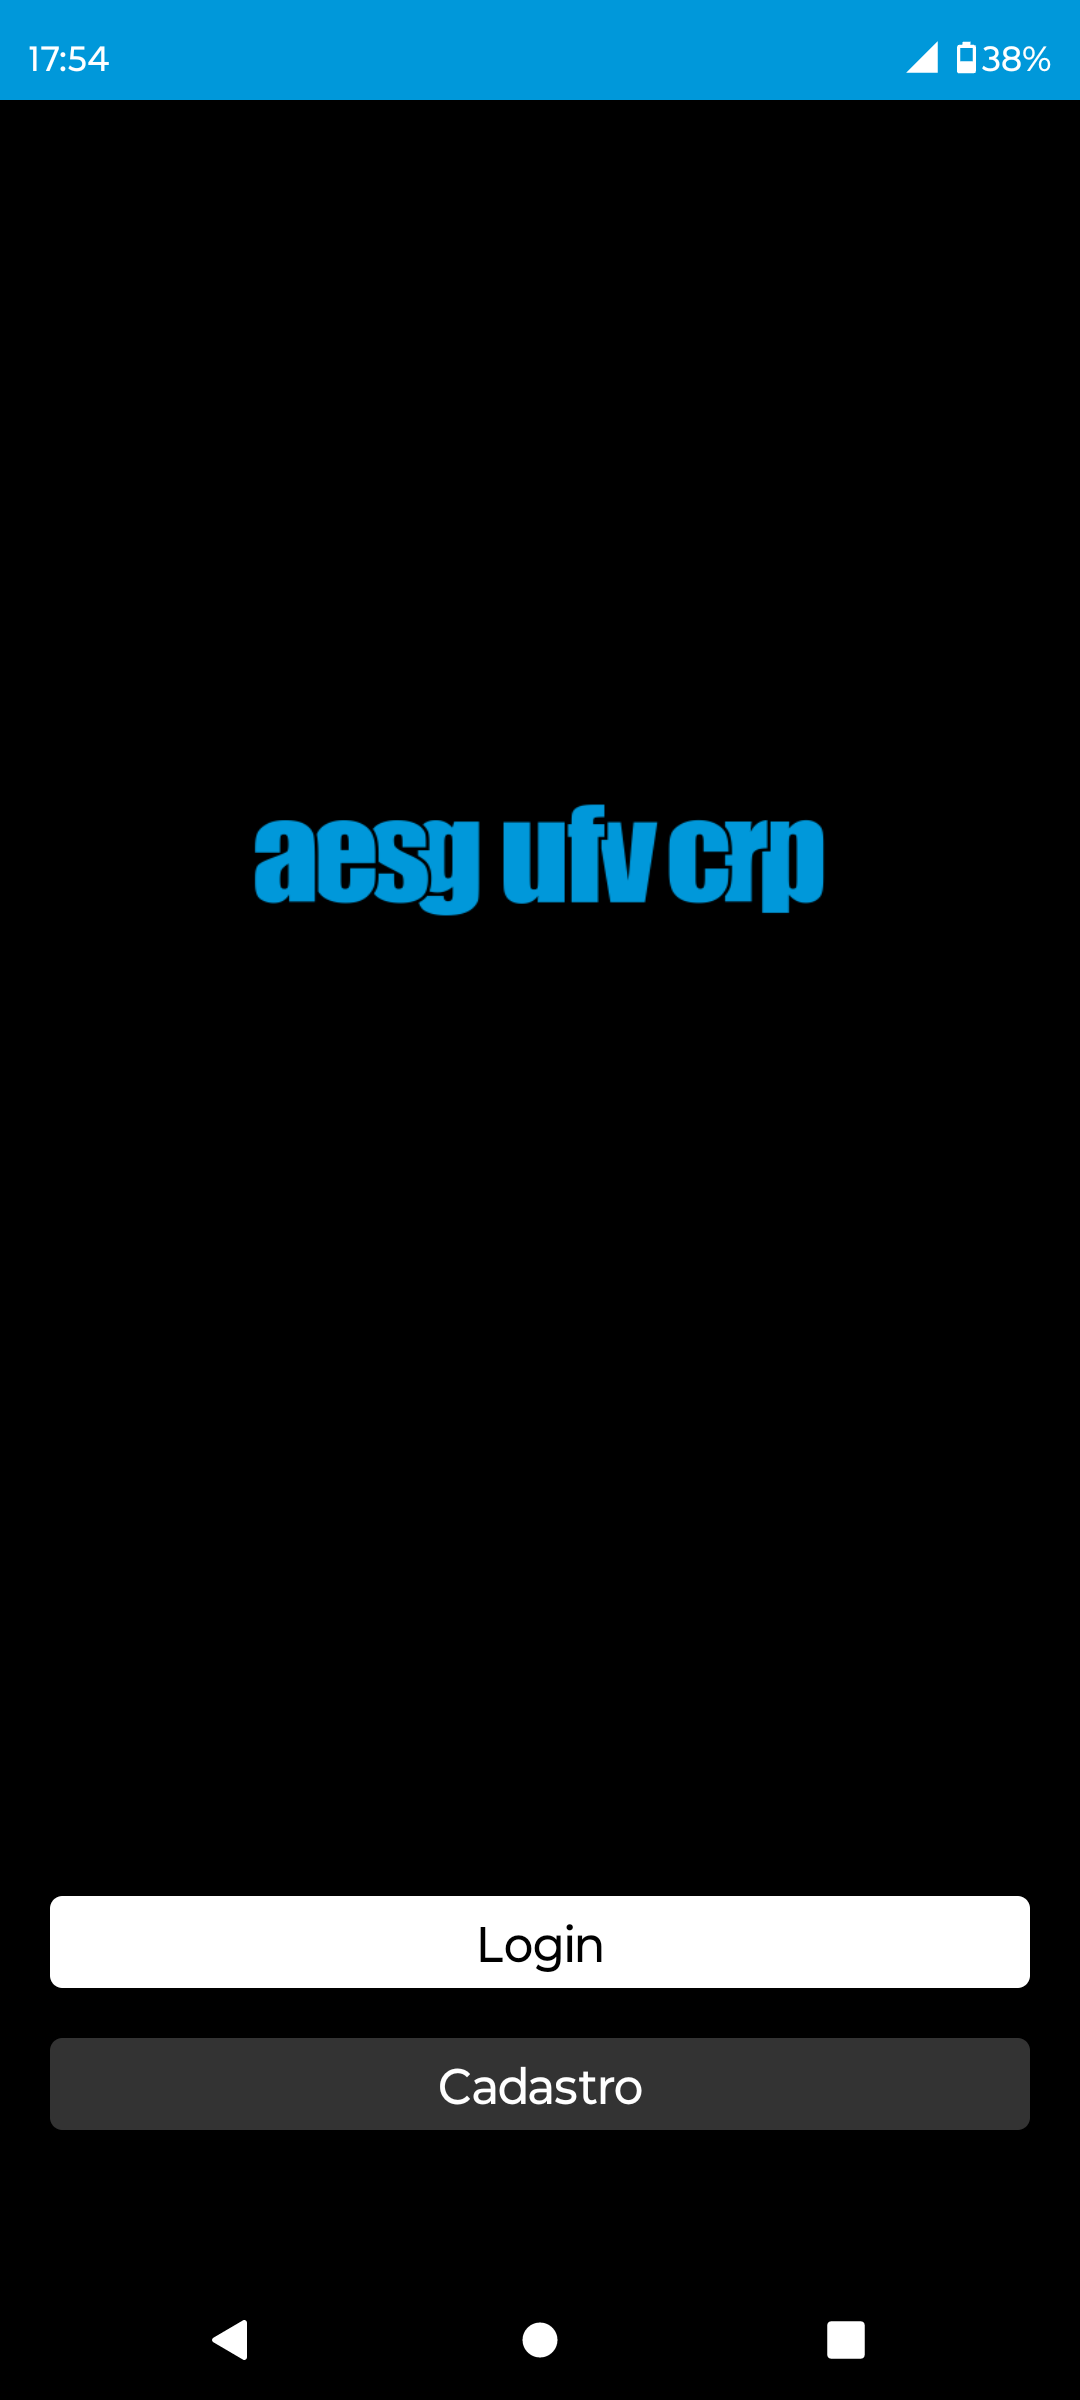
\includegraphics[width=0.4\linewidth]{Imagens/App Images          User/AU1.png}
                \end{center}
                \caption[Imagem da Tela Inicial do Aplicativo AESG]{ 
                Imagem da Tela Inicial do Aplicativo AESG}
                \label{fig:AppTelaInicial}
                \legend{Fonte: O author}
            \end{figure}
            
        \subsection{Tela de Login}
            A tela de Login vai ser acessada pelo usuario ao clicar no botão login na tela inicial, esta tela tem um cabecalho com o nome da pagina no topo, no corpo da pagina temos a logo em cor branca, e logo abaixo os campos de email e senha para que o usaurio possa fazer o login, apos prençher os dados corretamente ele devera clicar no botão entrar para efetuar seu login, porem se ele perceber que le não possui cadastro, ele pode acessar a tela de cadastro diretamente por esta pagina clicando no botão cadastrar-se a tela pode ser vista na Figura \ref{fig:AppTelaLogin}.
            \begin{figure}[!h]
                \begin{center}
                \centering
                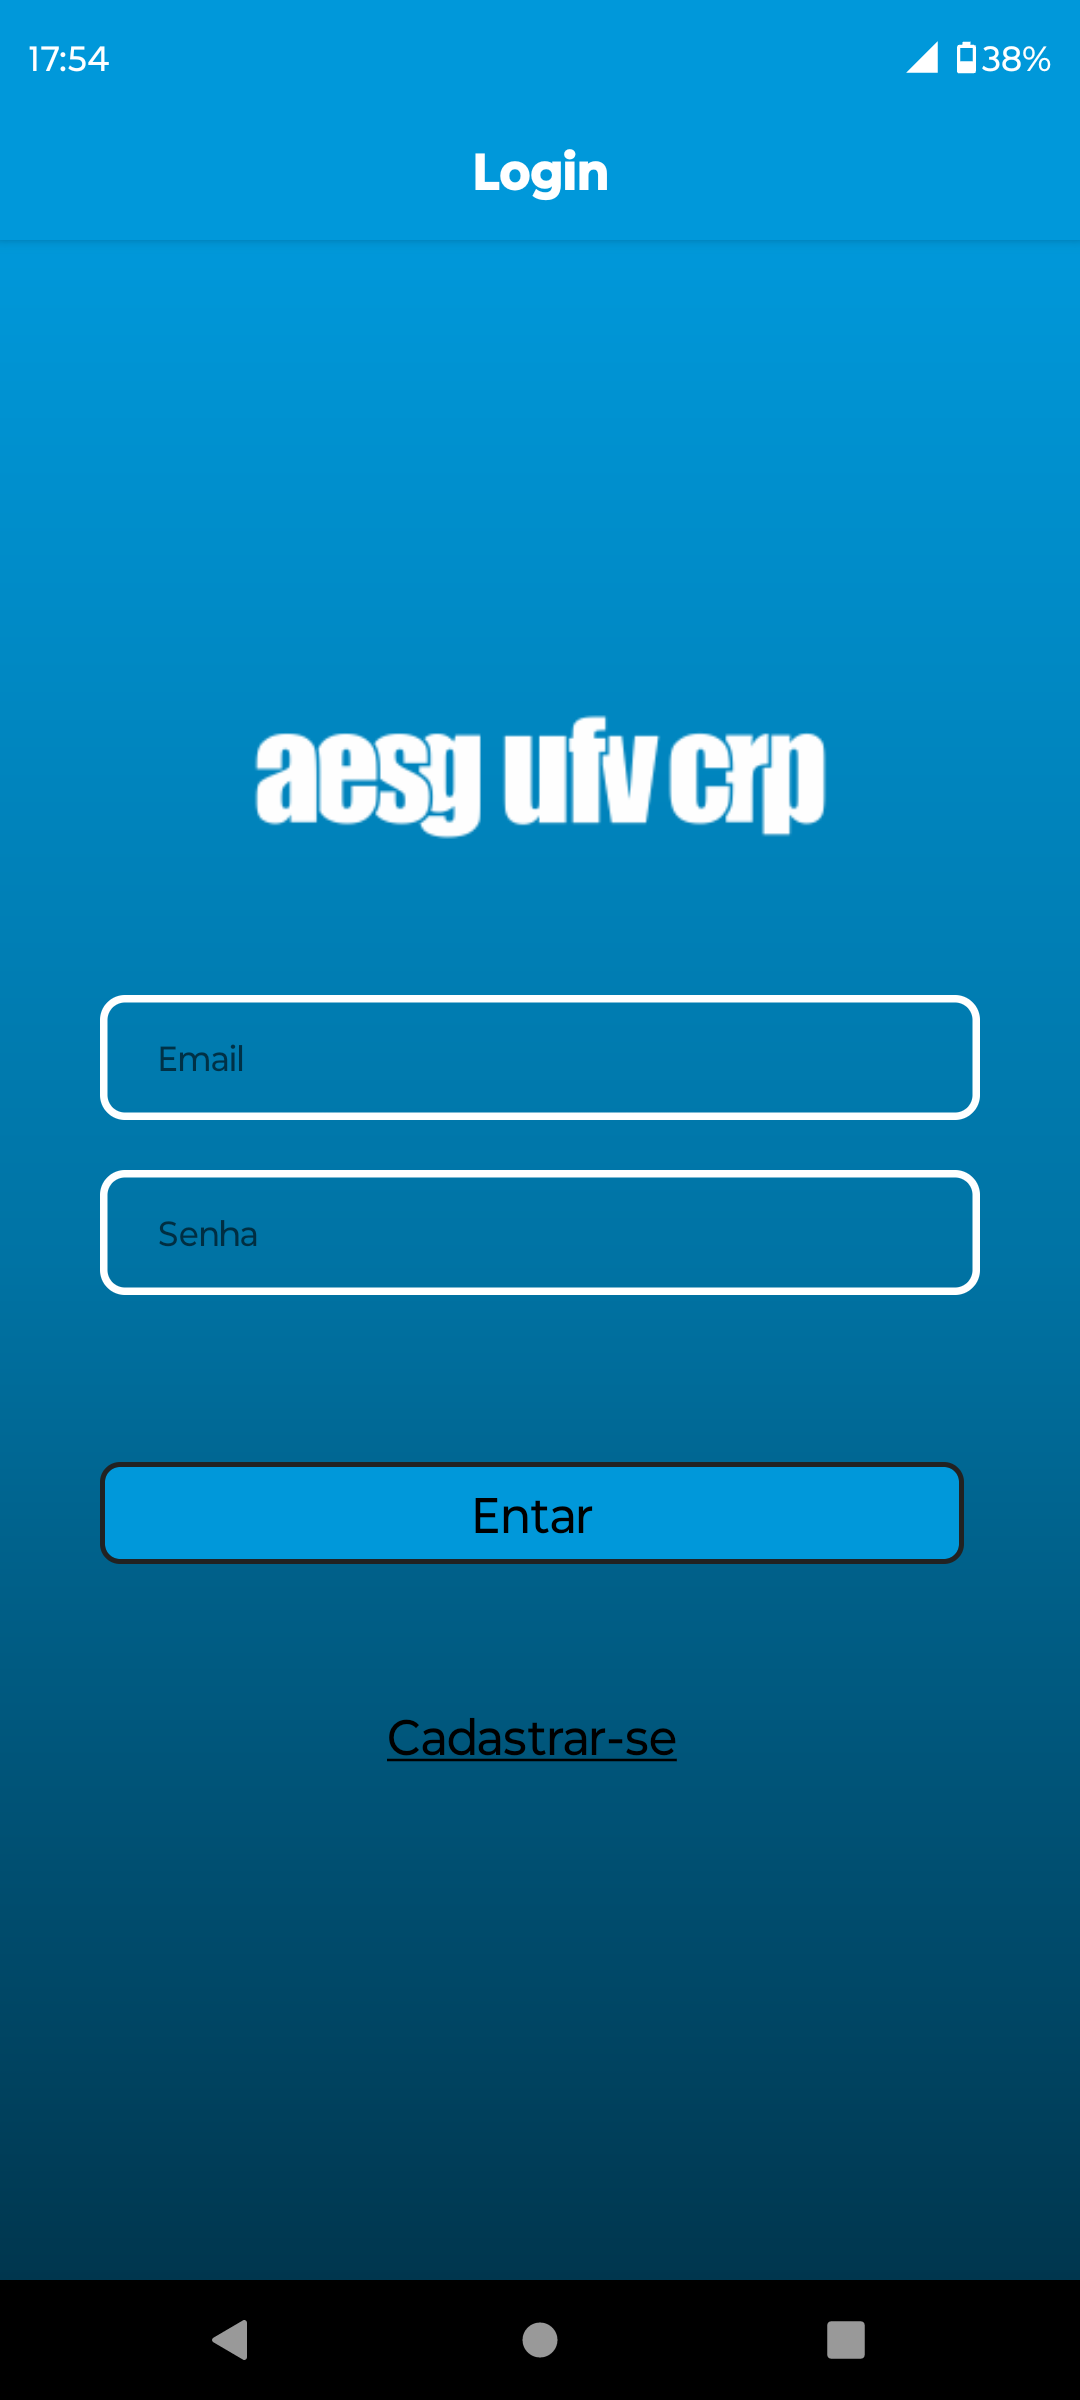
\includegraphics[width=0.4\linewidth]{Imagens/App Images          User/AU2.png}
                \end{center}
                \caption[Imagem da Tela de Login do Aplicativo AESG]{ 
                Imagem da Tela de Login do Aplicativo AESG}
                \label{fig:AppTelaLogin}
                \legend{Fonte: O author}
            \end{figure}
        \subsection{Tela de Cadastro}
            A tela de Cadastro vai ser acessada pelo usuario ao clicar no botão Cadastro na tela inicial ou no botão Cadastrar-se na tela de Login, esta tela tem uma estrutura diferente pois ela e composta de 7 telas, que fazem um cadastro guiado do usuario separada em 6 etapas, na preimeira etapa o usuario ira cadastrar seus dados de login, que são o email, senha e confirmar senha, tendo um botão mostrar senha para o usuario conferir se digitou corretamente, e na parte inferior um botão para avnçar para a proxima estapa, a tela pode ser vista na Figura \ref{fig:AppTelaCadastro10} e Figura \ref{fig:AppTelaCadastro1}.
            \begin{figure}[!h]          
                \begin{minipage}{0.5\textwidth}
                    \centering
                    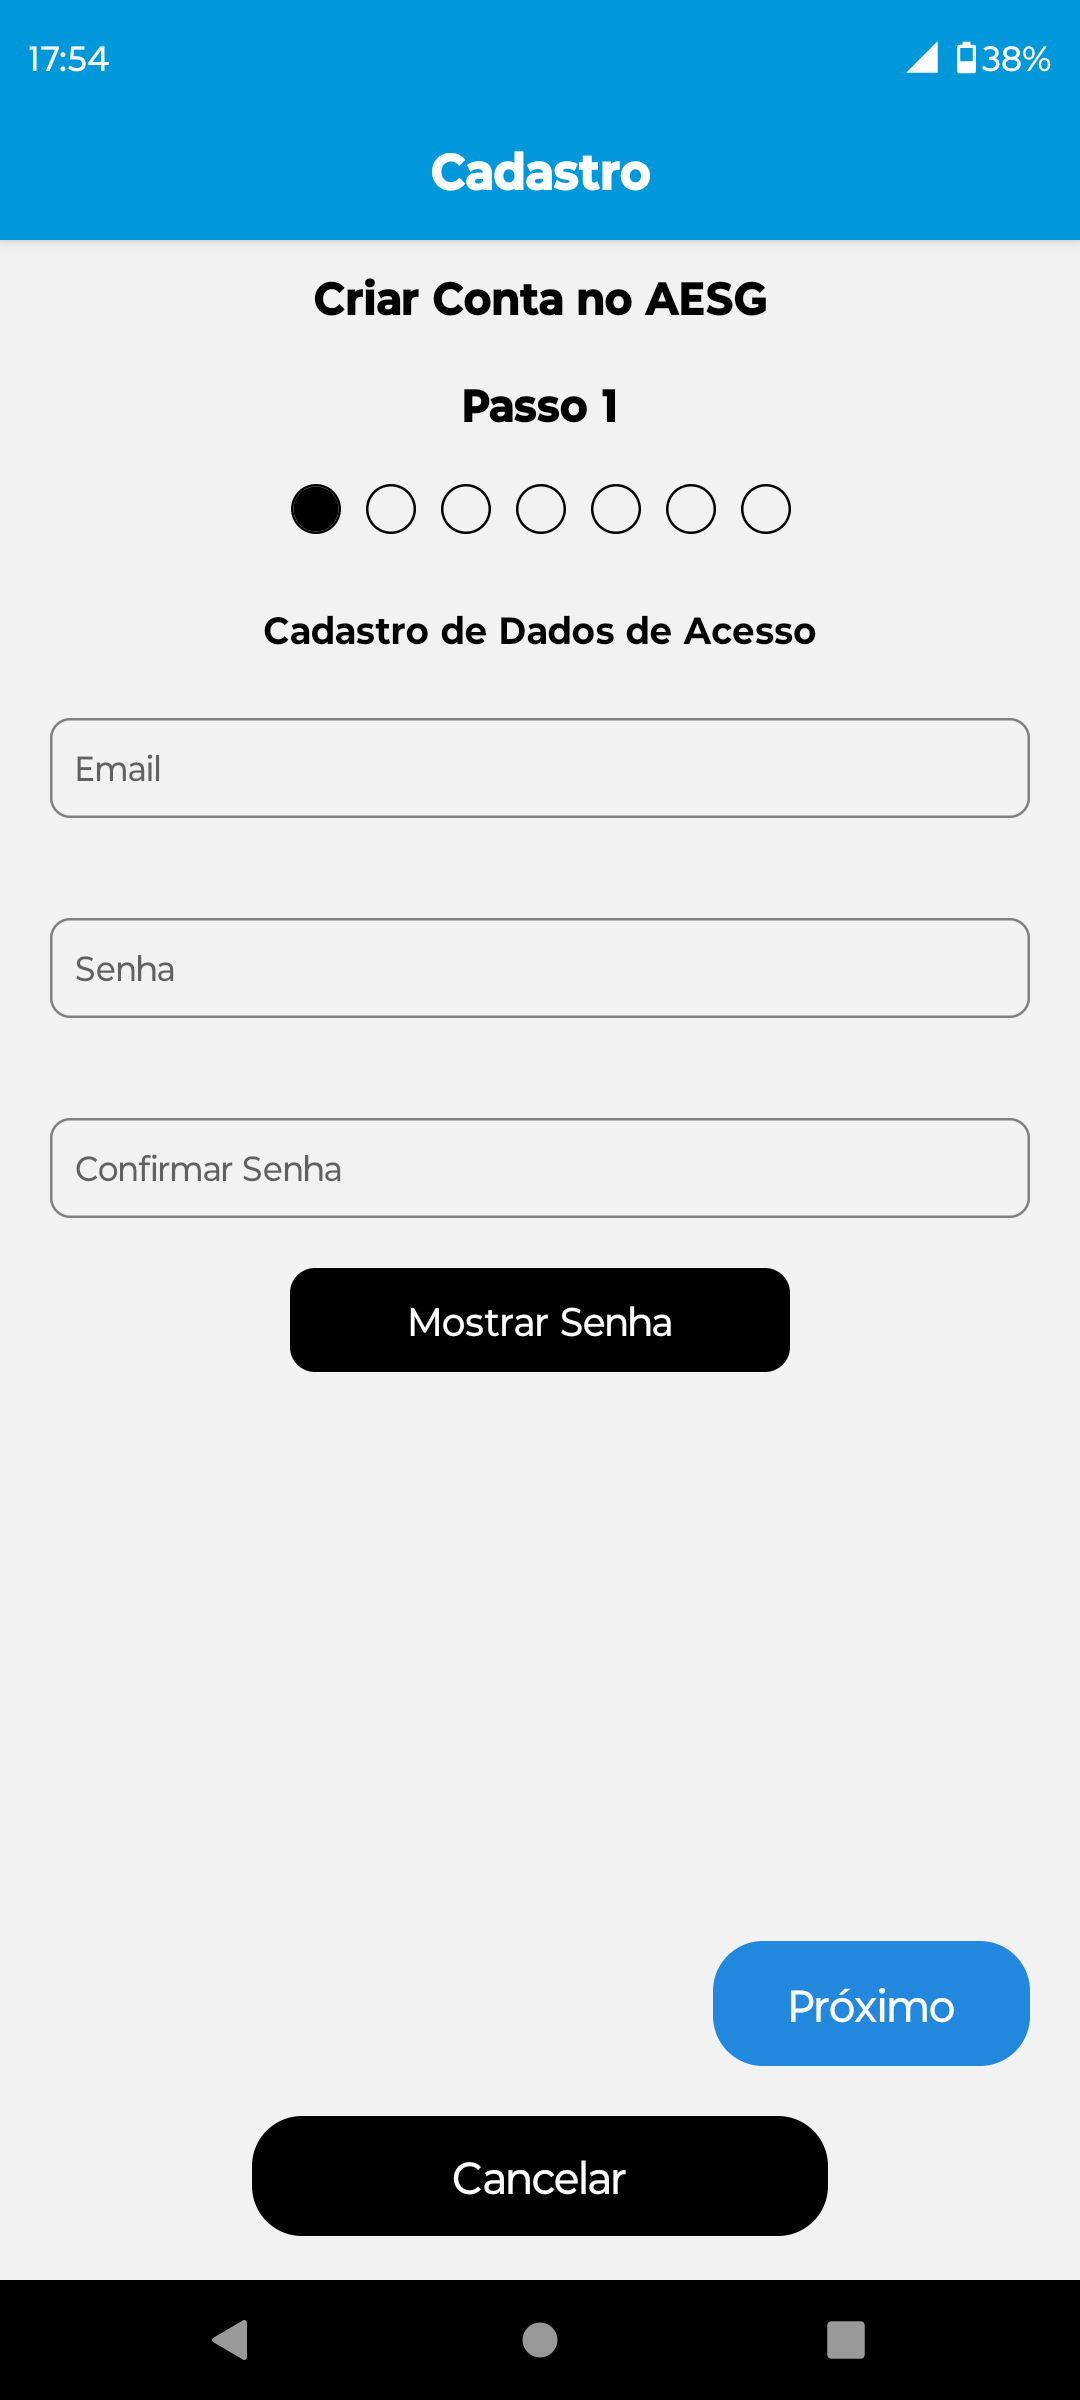
\includegraphics[width=0.8\linewidth]{Imagens/App Images User/AUCadastro10.png}
                    \caption[Imagem da Tela de Cadastro dos Dados de Acesso do Aplicativo AESG]{ 
                    Imagem da Tela de Cadastro dos Dados de Acesso do Aplicativo AESG}
                    \label{fig:AppTelaCadastro10}
                    \legend{Fonte: O author}
                \end{minipage}%
                \begin{minipage}{0.5\textwidth}
                    \centering
                    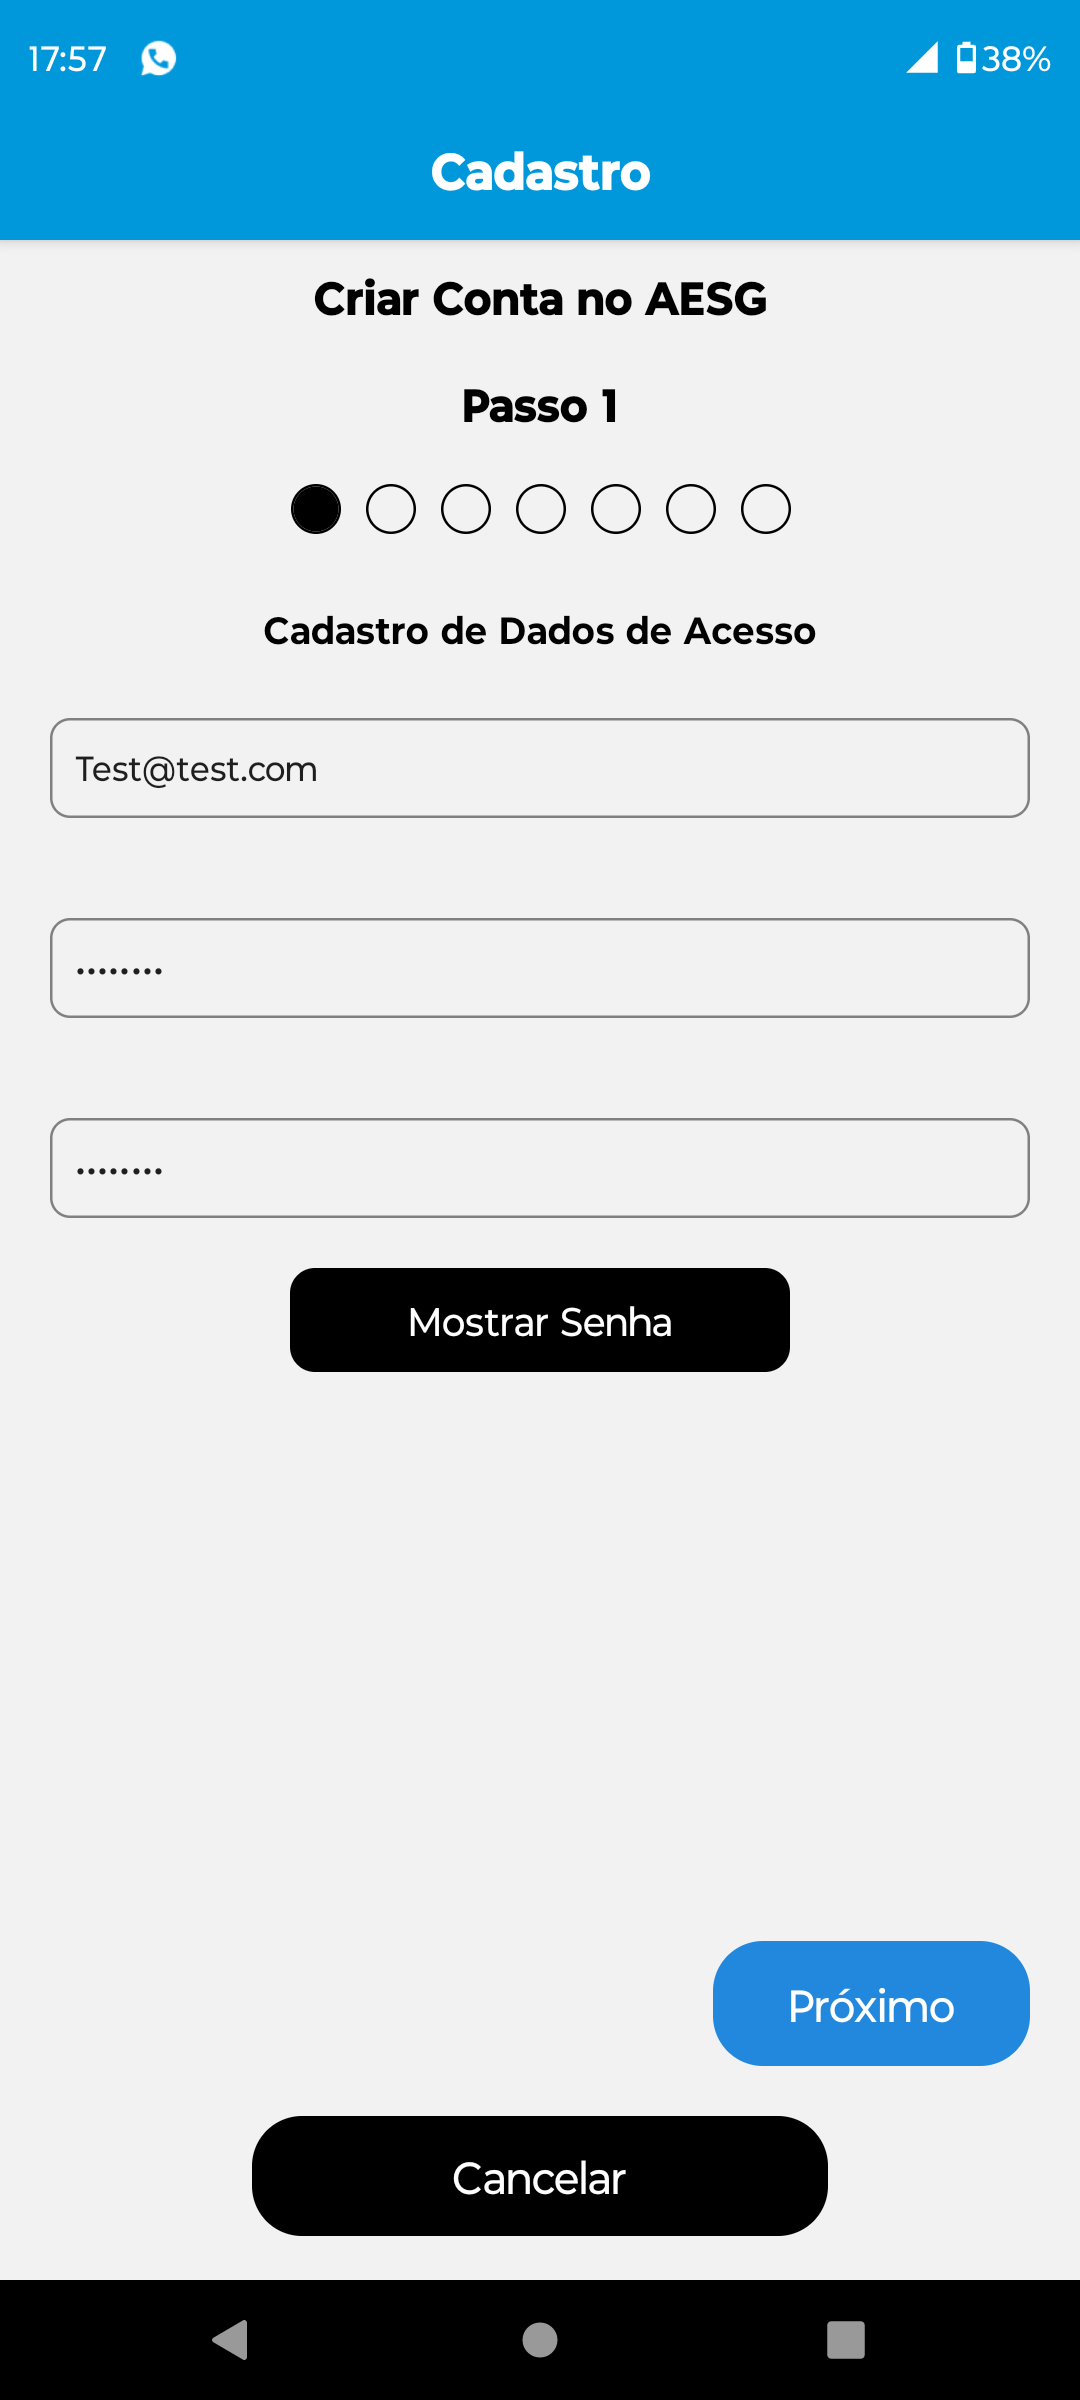
\includegraphics[width=0.8\linewidth]{Imagens/App Images User/AUCadastro1.png}
                    \caption[Imagem da Tela de Cadastro dos Dados de Acesso Preenchido do Aplicativo AESG]{ 
                    Imagem da Tela de Cadastro dos Dados de Acesso do Aplicativo AESG}
                    \label{fig:AppTelaCadastro1}
                    \legend{Fonte: O author}
                \end{minipage}
            \end{figure}

            \newpage
            
            Na tela do passo 2 o Usuario ira cadastrar seus dados pessoais como nome, celular, CPF e data de nacimento, na parte inferir da tela ele tera opçoes para voltar para o passo aonterios ou proseguir para o seguinte, a tela pode ser vista na Figura \ref{fig:AppTelaCadastro11} e Figura \ref{fig:AppTelaCadastro2}.   
            \begin{figure}[!h]          
                \begin{minipage}{0.5\textwidth}
                    \centering
                    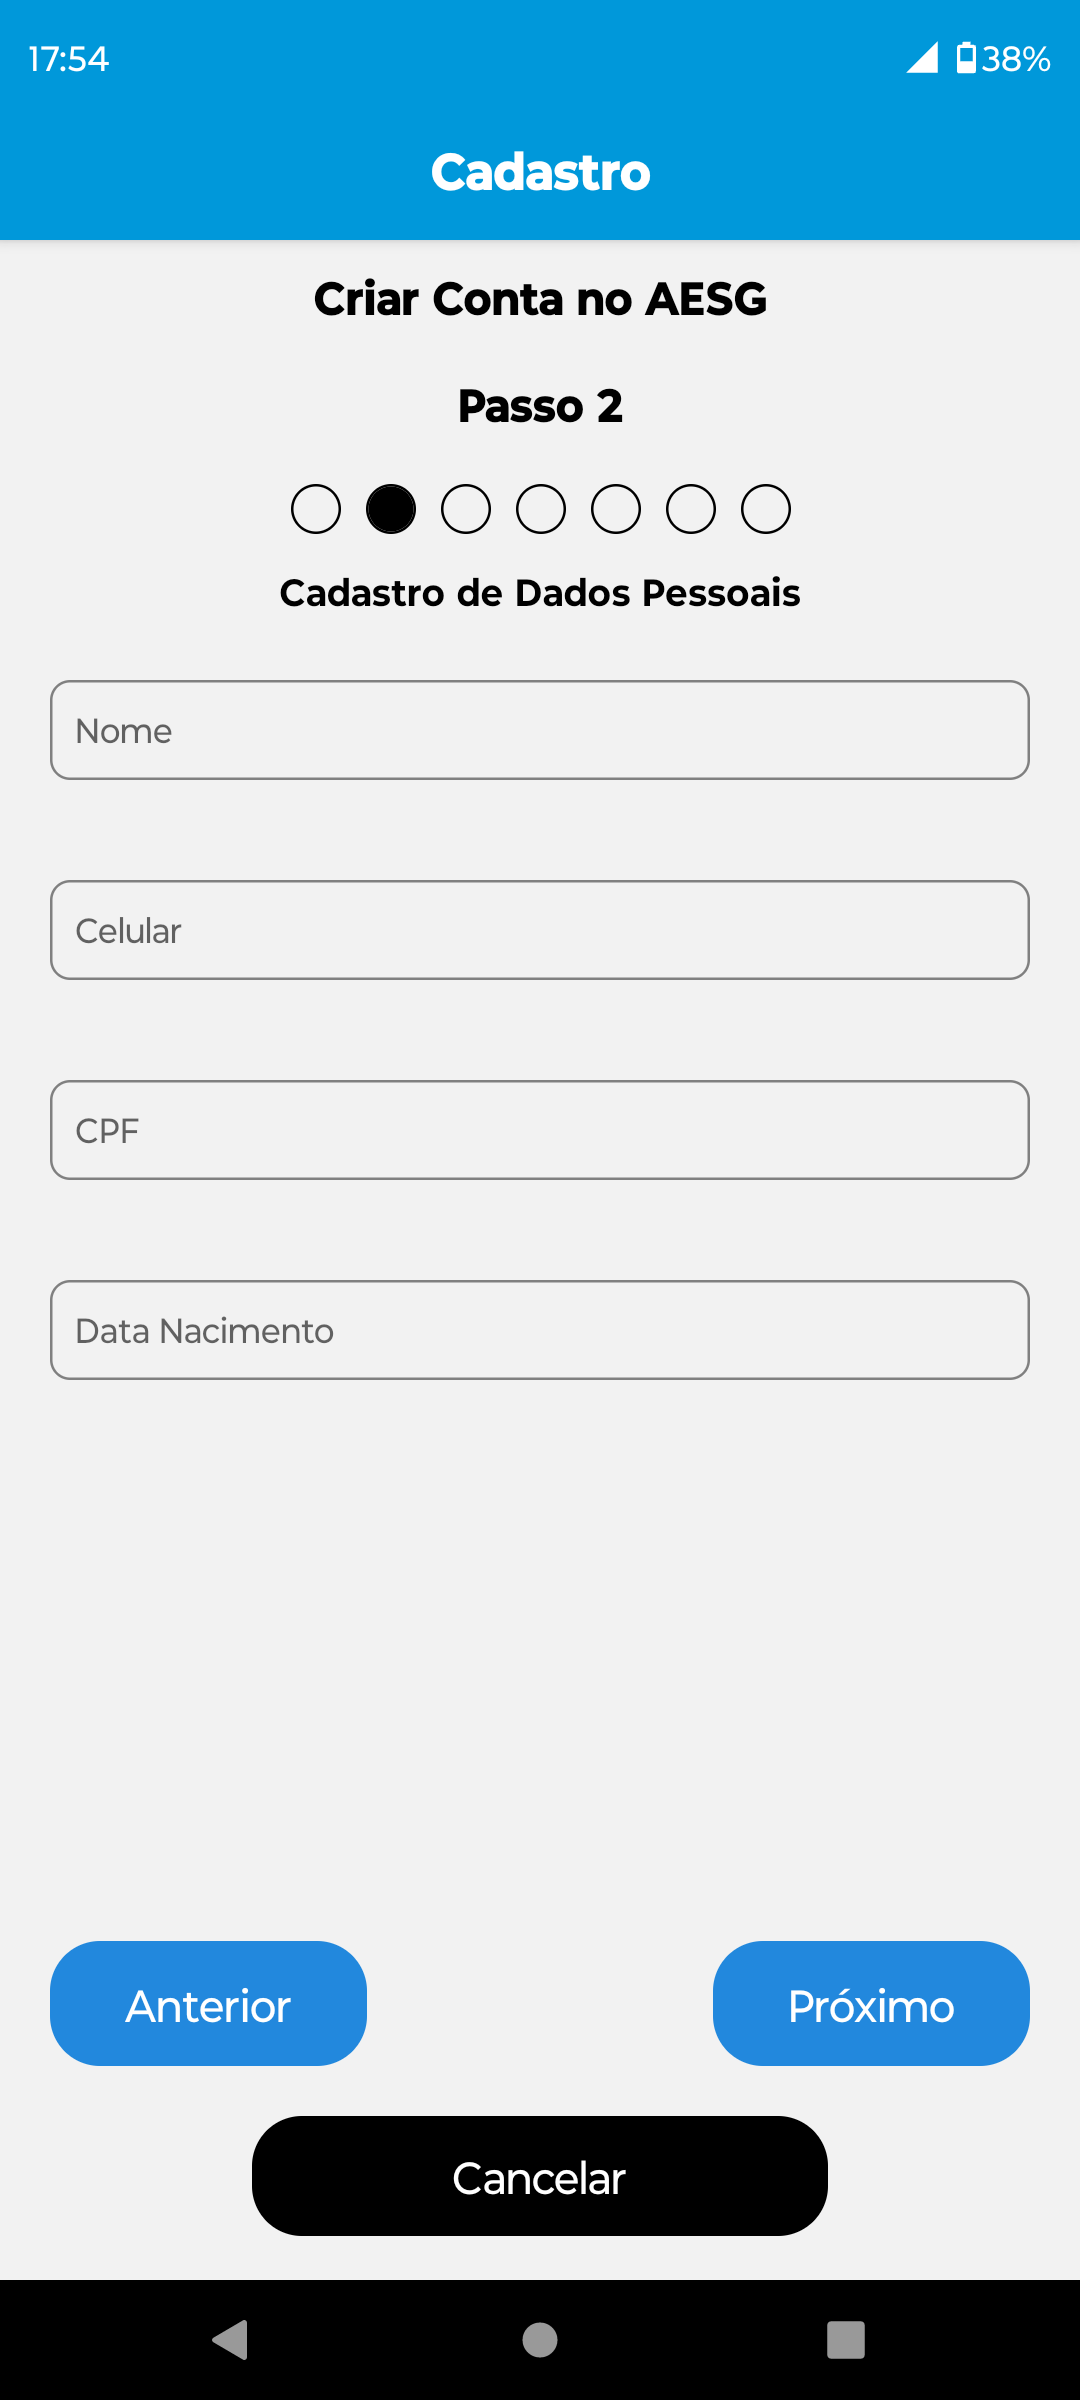
\includegraphics[width=0.8\linewidth]{Imagens/App Images User/AUCadastro11.png}
                    \caption[Imagem da Tela de Cadastro dos Dados Pessoais do Aplicativo AESG]{ 
                    Imagem da Tela de Cadastro dos Dados de Acesso do Aplicativo AESG}
                    \label{fig:AppTelaCadastro11}
                    \legend{Fonte: O author}
                \end{minipage}%
                \begin{minipage}{0.5\textwidth}
                    \centering
                    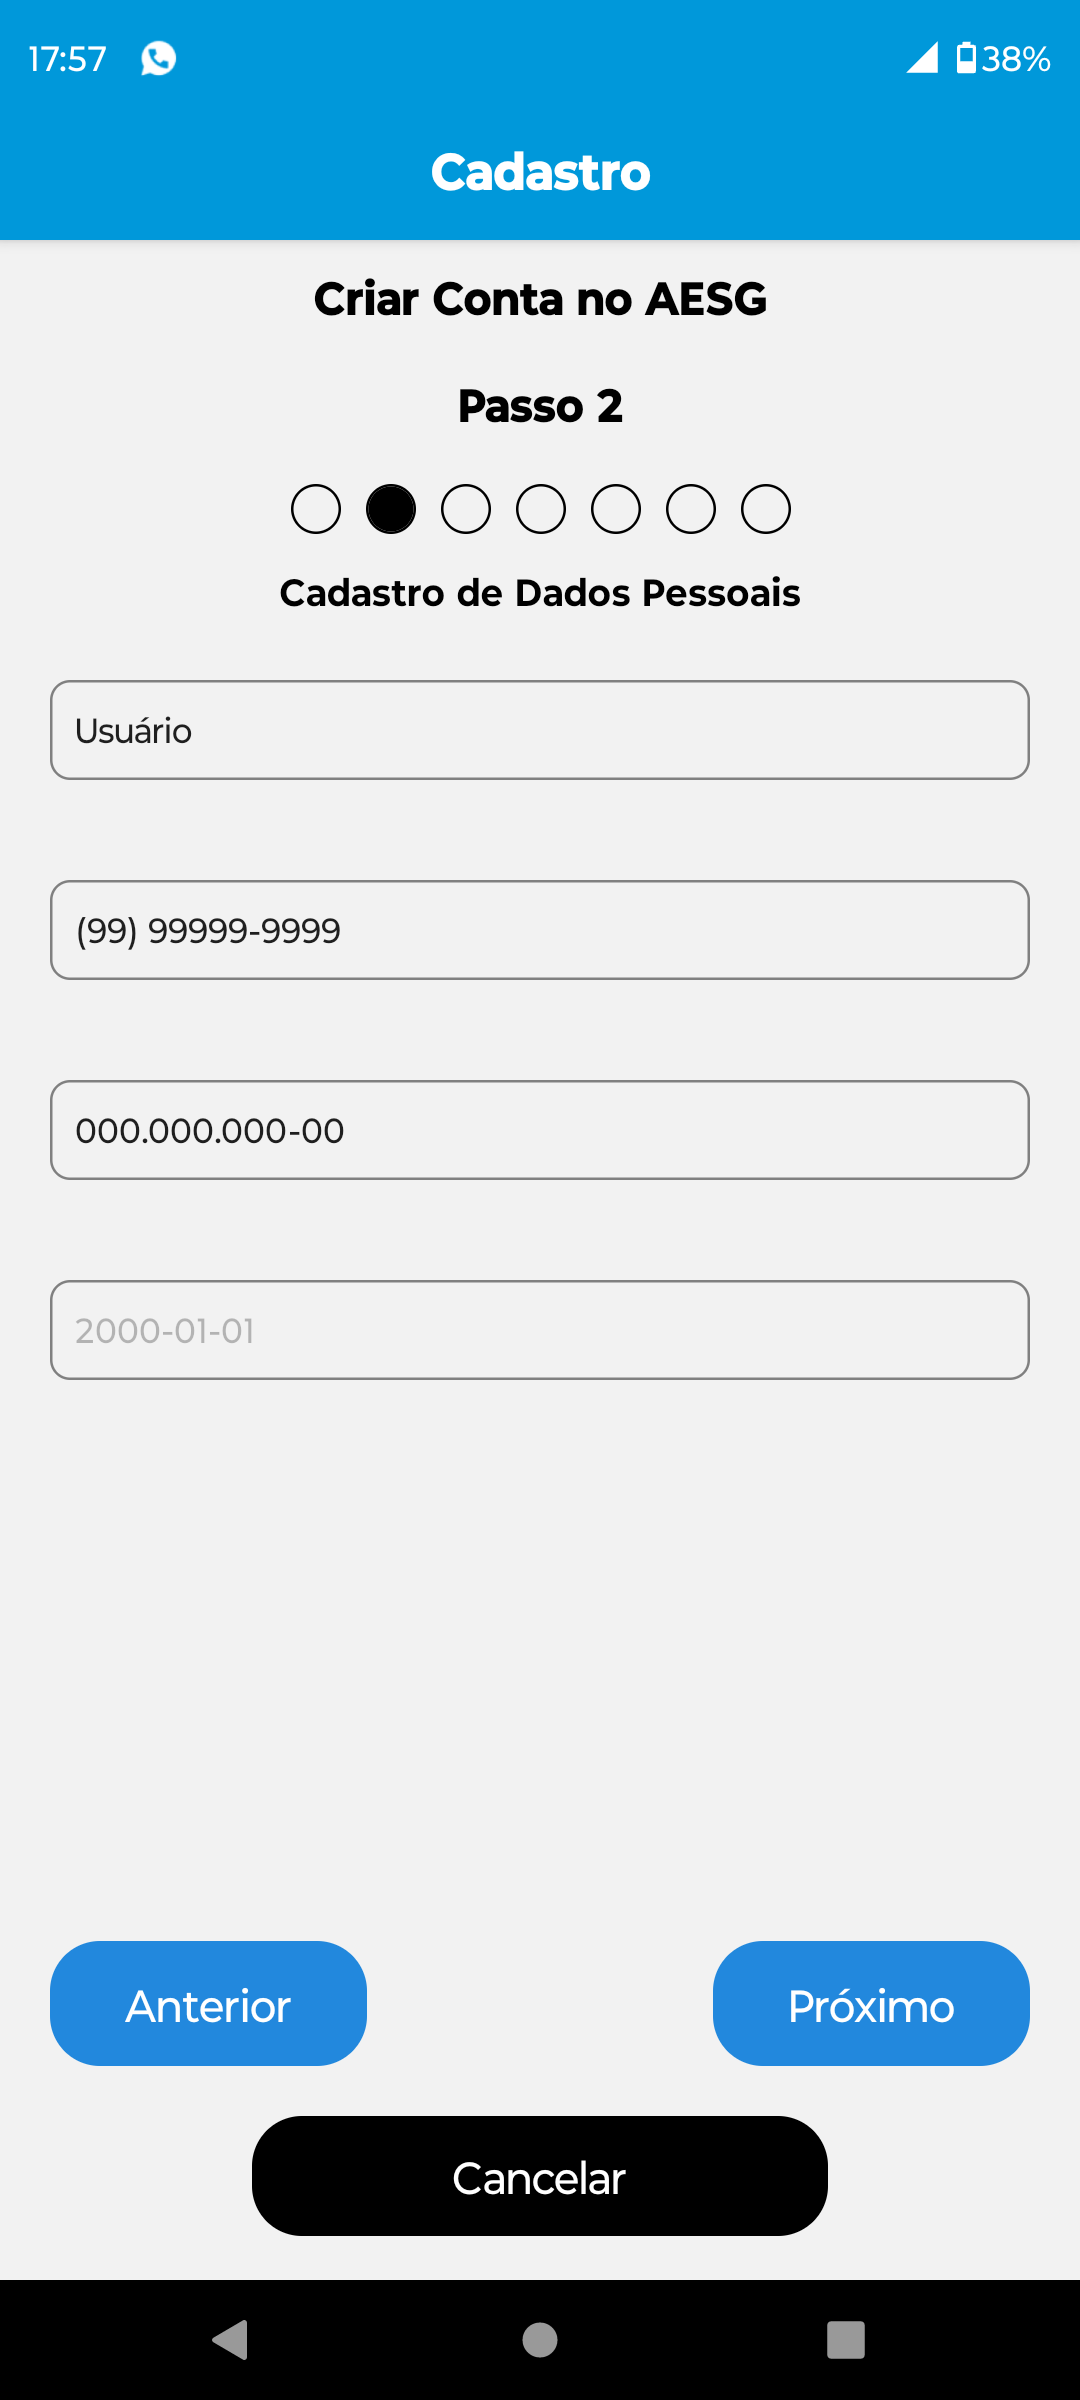
\includegraphics[width=0.8\linewidth]{Imagens/App Images User/AUCadastro2.png}
                    \caption[Imagem da Tela de Cadastro dos Dados de Pessoais Preenchido do Aplicativo AESG]{ 
                    Imagem da Tela de Cadastro dos Dados de Acesso do Aplicativo AESG}
                    \label{fig:AppTelaCadastro2}
                    \legend{Fonte: O author}
                \end{minipage}
            \end{figure}

            \newpage
            Na tela do passo 3 o Usuário ira cadastrar seus dados de endereço como cidade, estado, bairro, rua e numero  da casa, na parte inferir da tela ele tera opções para voltar para o passo anterior ou prosseguir para o seguinte, a tela pode ser vista na Figura \ref{fig:AppTelaCadastro12} e Figura \ref{fig:AppTelaCadastro3}.
            \begin{figure}[!h]          
                \begin{minipage}{0.5\textwidth}
                    \centering
                    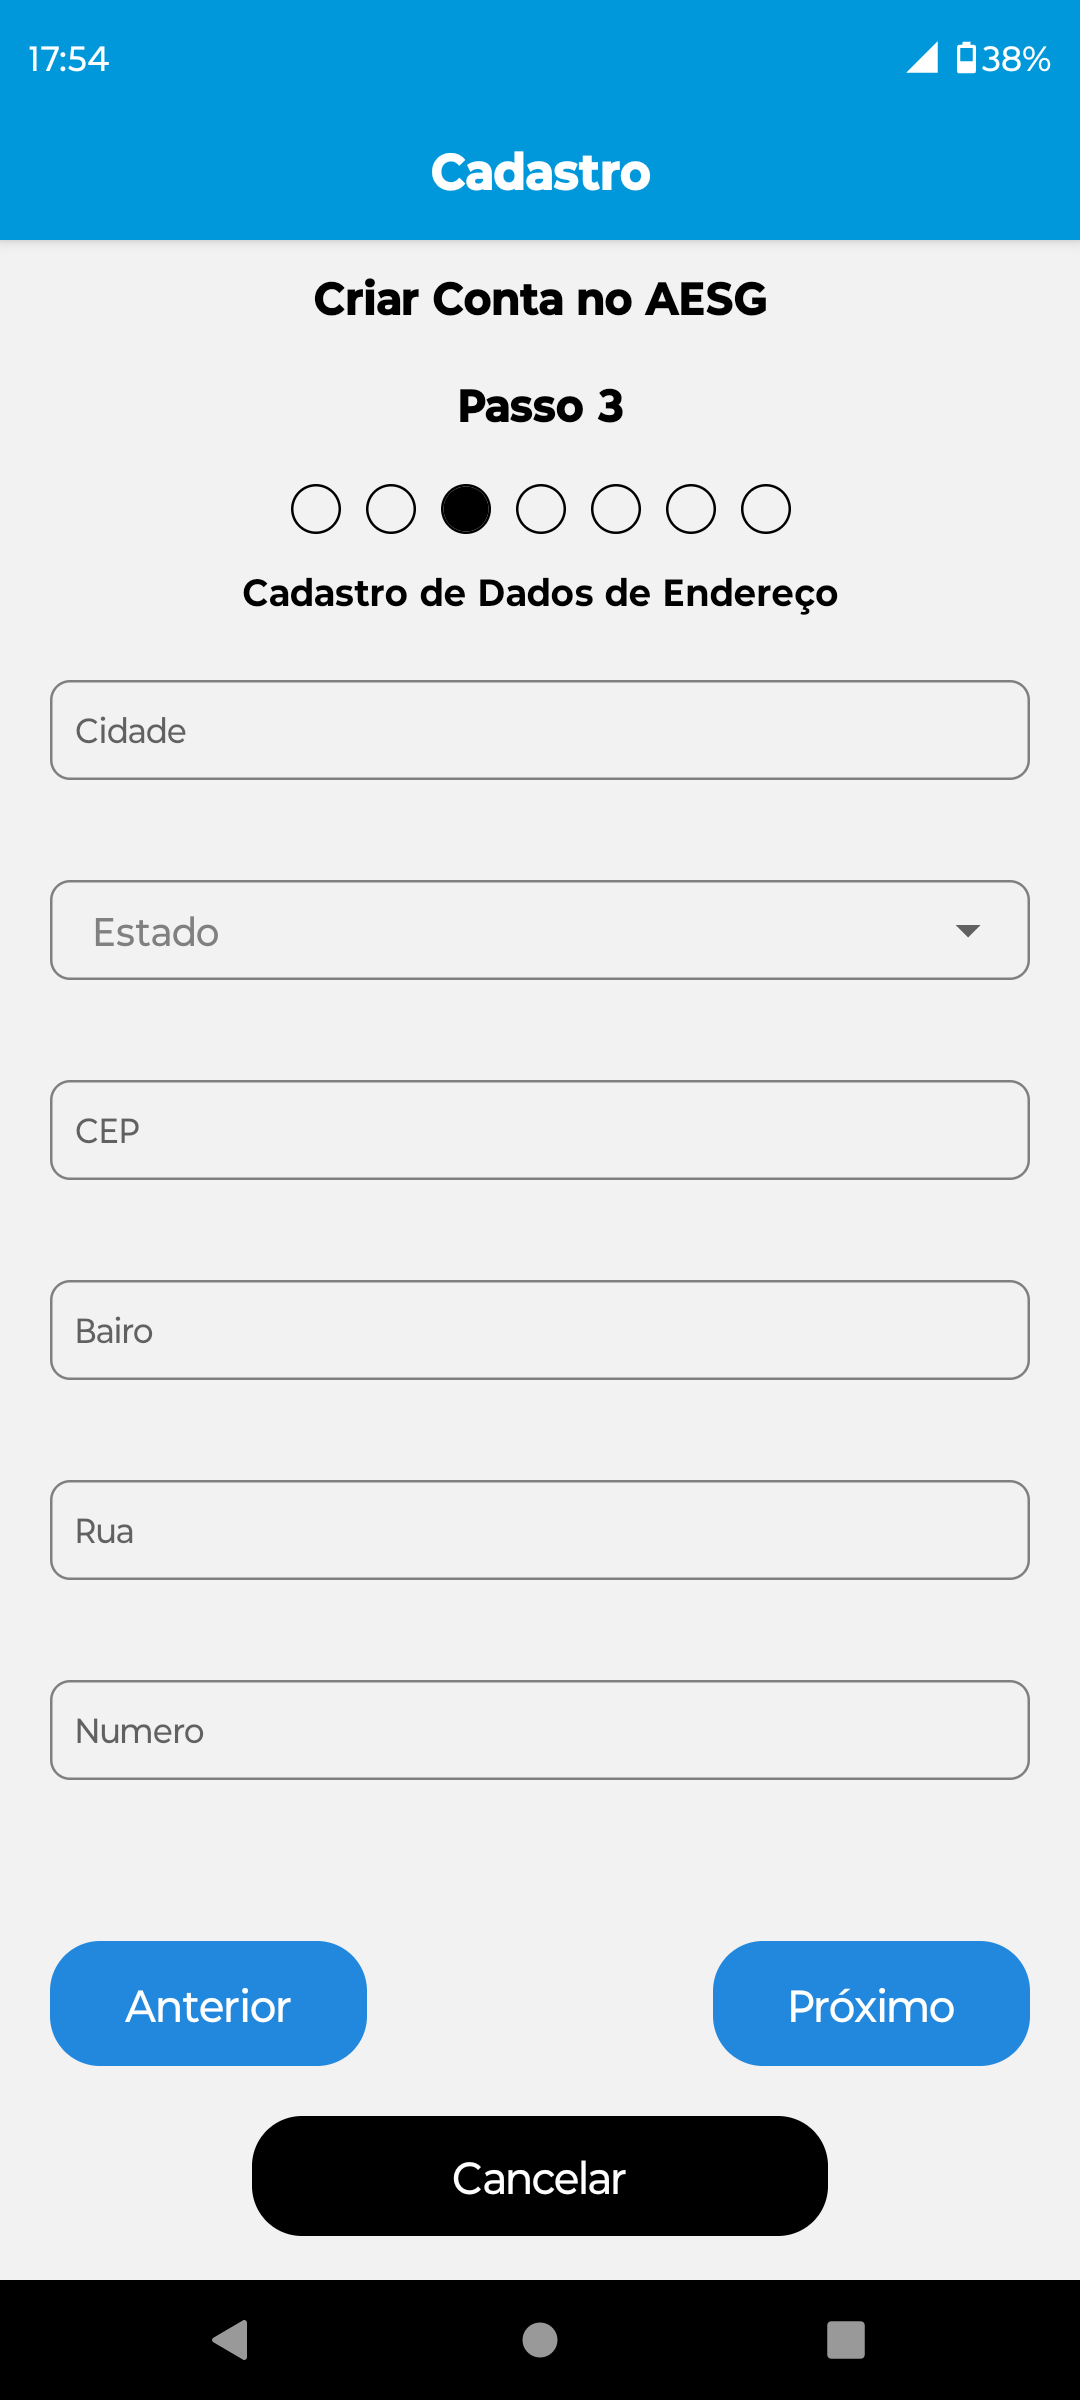
\includegraphics[width=0.8\linewidth]{Imagens/App Images User/AUCadastro12.png}
                    \caption[Imagem da Tela de Cadastro dos Dados de Endereço do Aplicativo AESG]{ 
                    Imagem da Tela de Cadastro dos Dados de Endereço do Aplicativo AESG}
                    \label{fig:AppTelaCadastro12}
                    \legend{Fonte: O author}
                \end{minipage}%
                \begin{minipage}{0.5\textwidth}
                    \centering
                    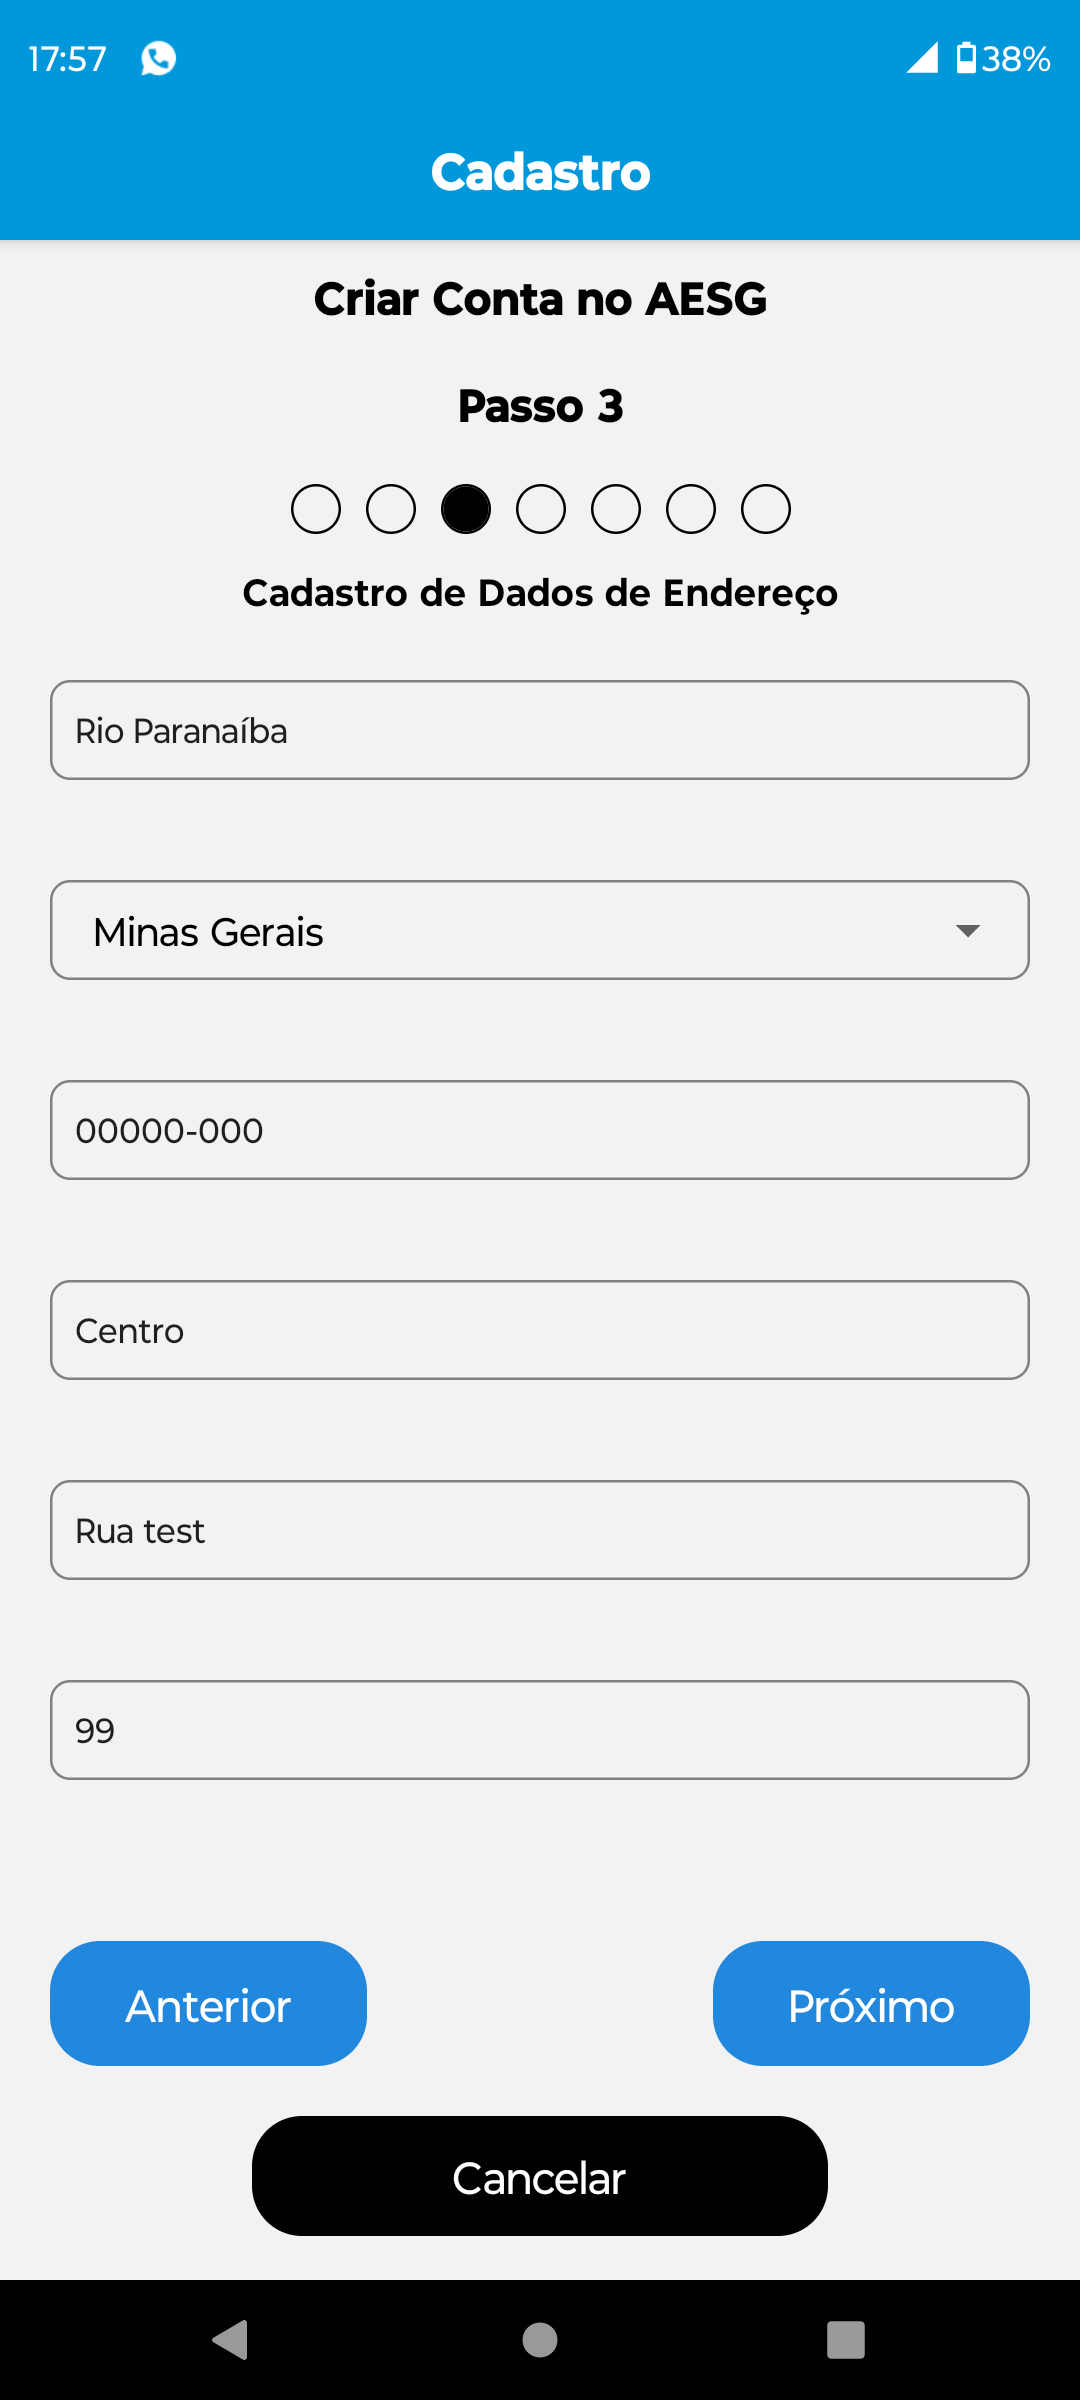
\includegraphics[width=0.8\linewidth]{Imagens/App Images User/AUCadastro3.png}
                    \caption[Imagem da Tela de Cadastro dos Dados de Endereço Preenchido do Aplicativo AESG]{ 
                    Imagem da Tela de Cadastro dos Dados de Endereço do Aplicativo AESG}
                    \label{fig:AppTelaCadastro3}
                    \legend{Fonte: O author}
                \end{minipage}
            \end{figure}
            \newpage
            Na tela do passo 4 o Usuário ira cadastrar seus dados da faculdade como matricula, curso, e ano de ingresso, na parte inferir da tela ele tera opções para voltar para o passo anterior ou prosseguir para o seguinte, a tela pode ser vista na Figura \ref{fig:AppTelaCadastro13} e Figura \ref{fig:AppTelaCadastro4}.
            \begin{figure}[!h]          
                \begin{minipage}{0.5\textwidth}
                    \centering
                    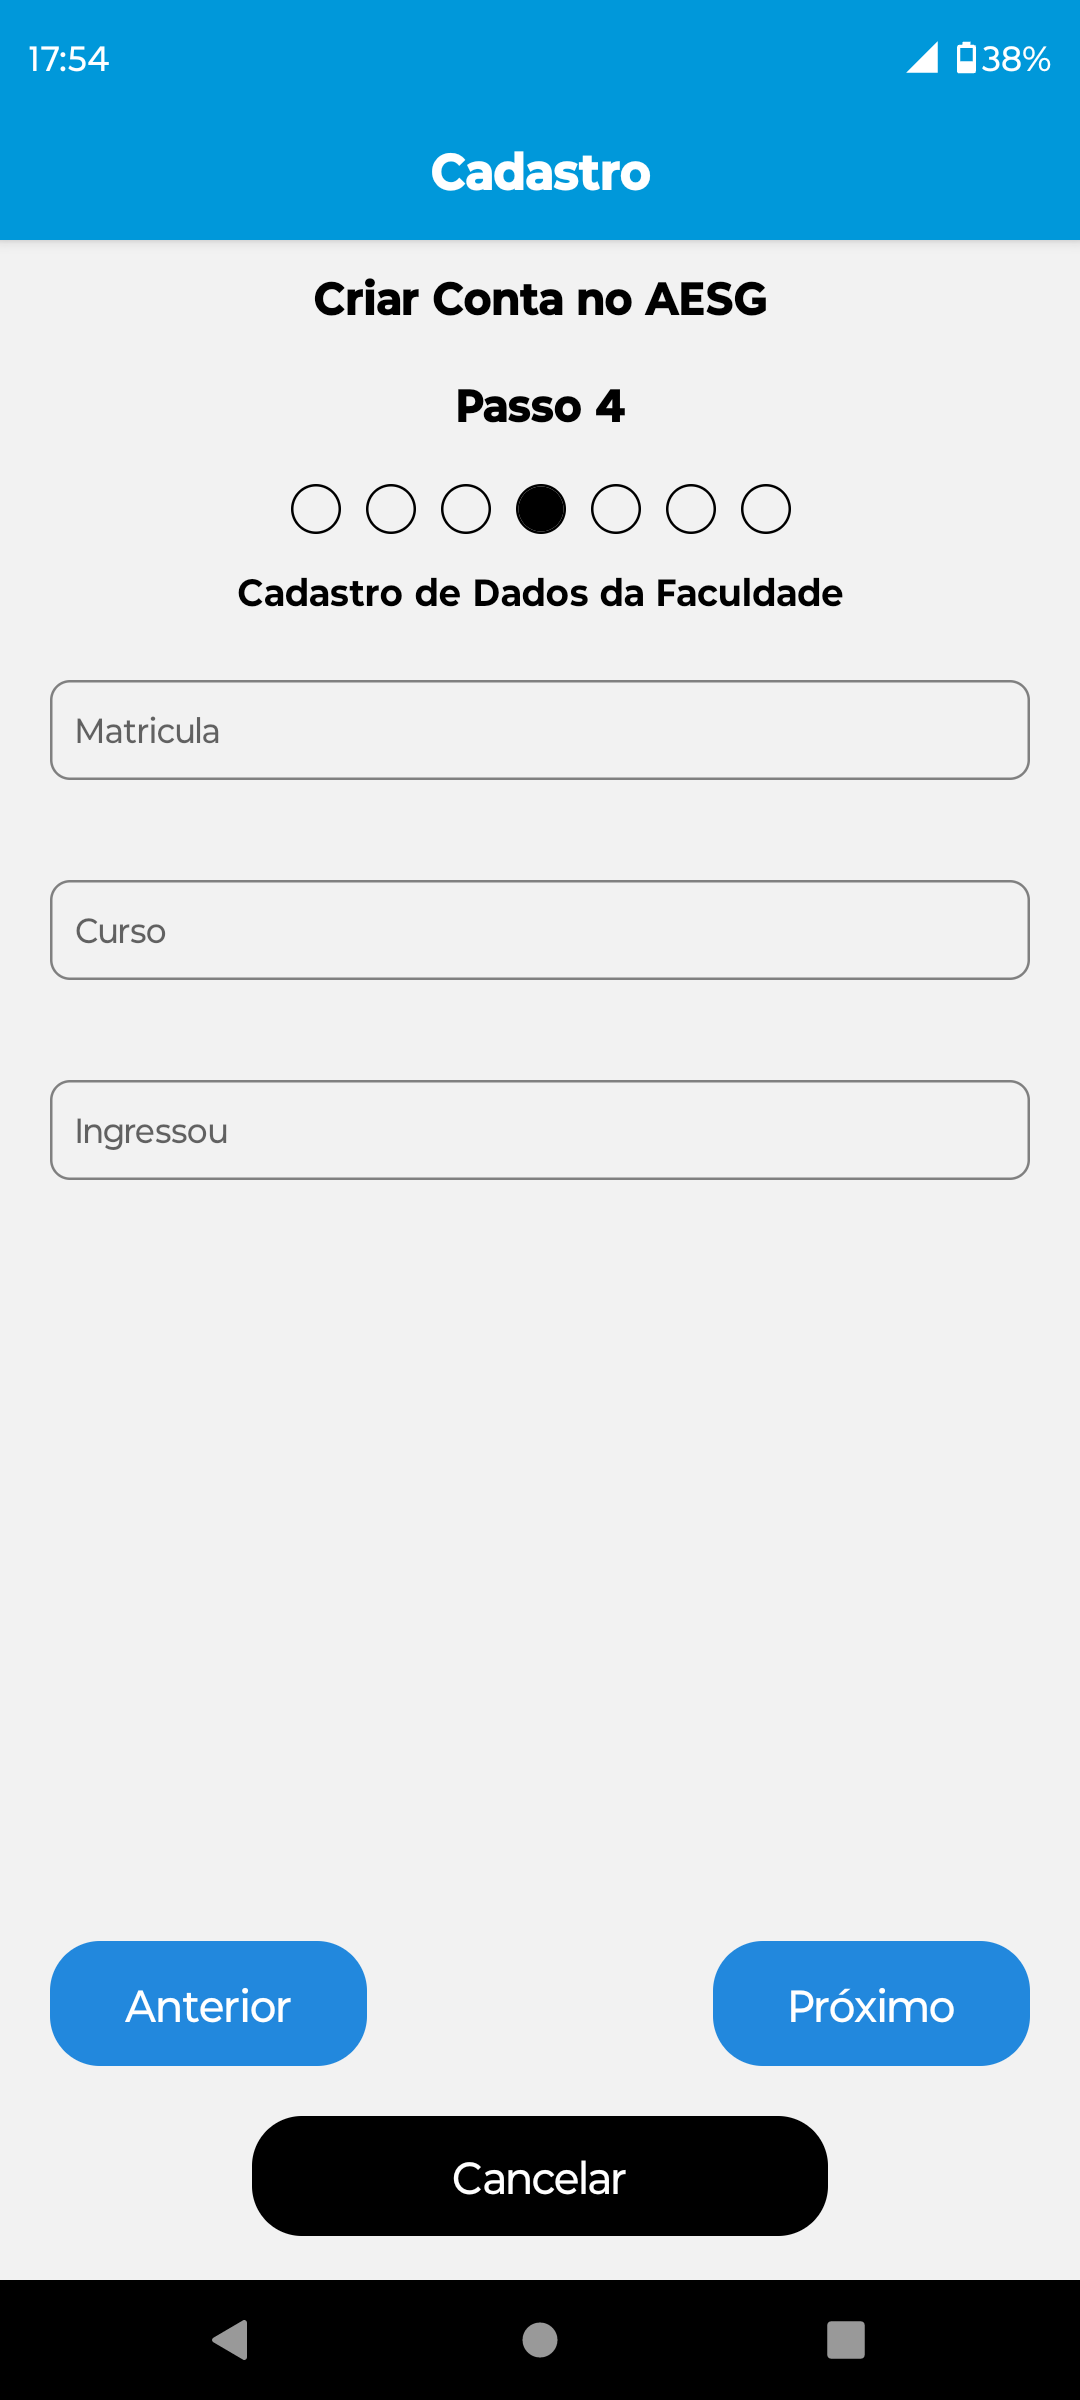
\includegraphics[width=0.8\linewidth]{Imagens/App Images User/AUCadastro13.png}
                    \caption[Imagem da Tela de Cadastro dos Dados da Faculdade do Aplicativo AESG]{ 
                    Imagem da Tela de Cadastro dos Dados da Faculdade do Aplicativo AESG}
                    \label{fig:AppTelaCadastro13}
                    \legend{Fonte: O author}
                \end{minipage}%
                \begin{minipage}{0.5\textwidth}
                    \centering
                    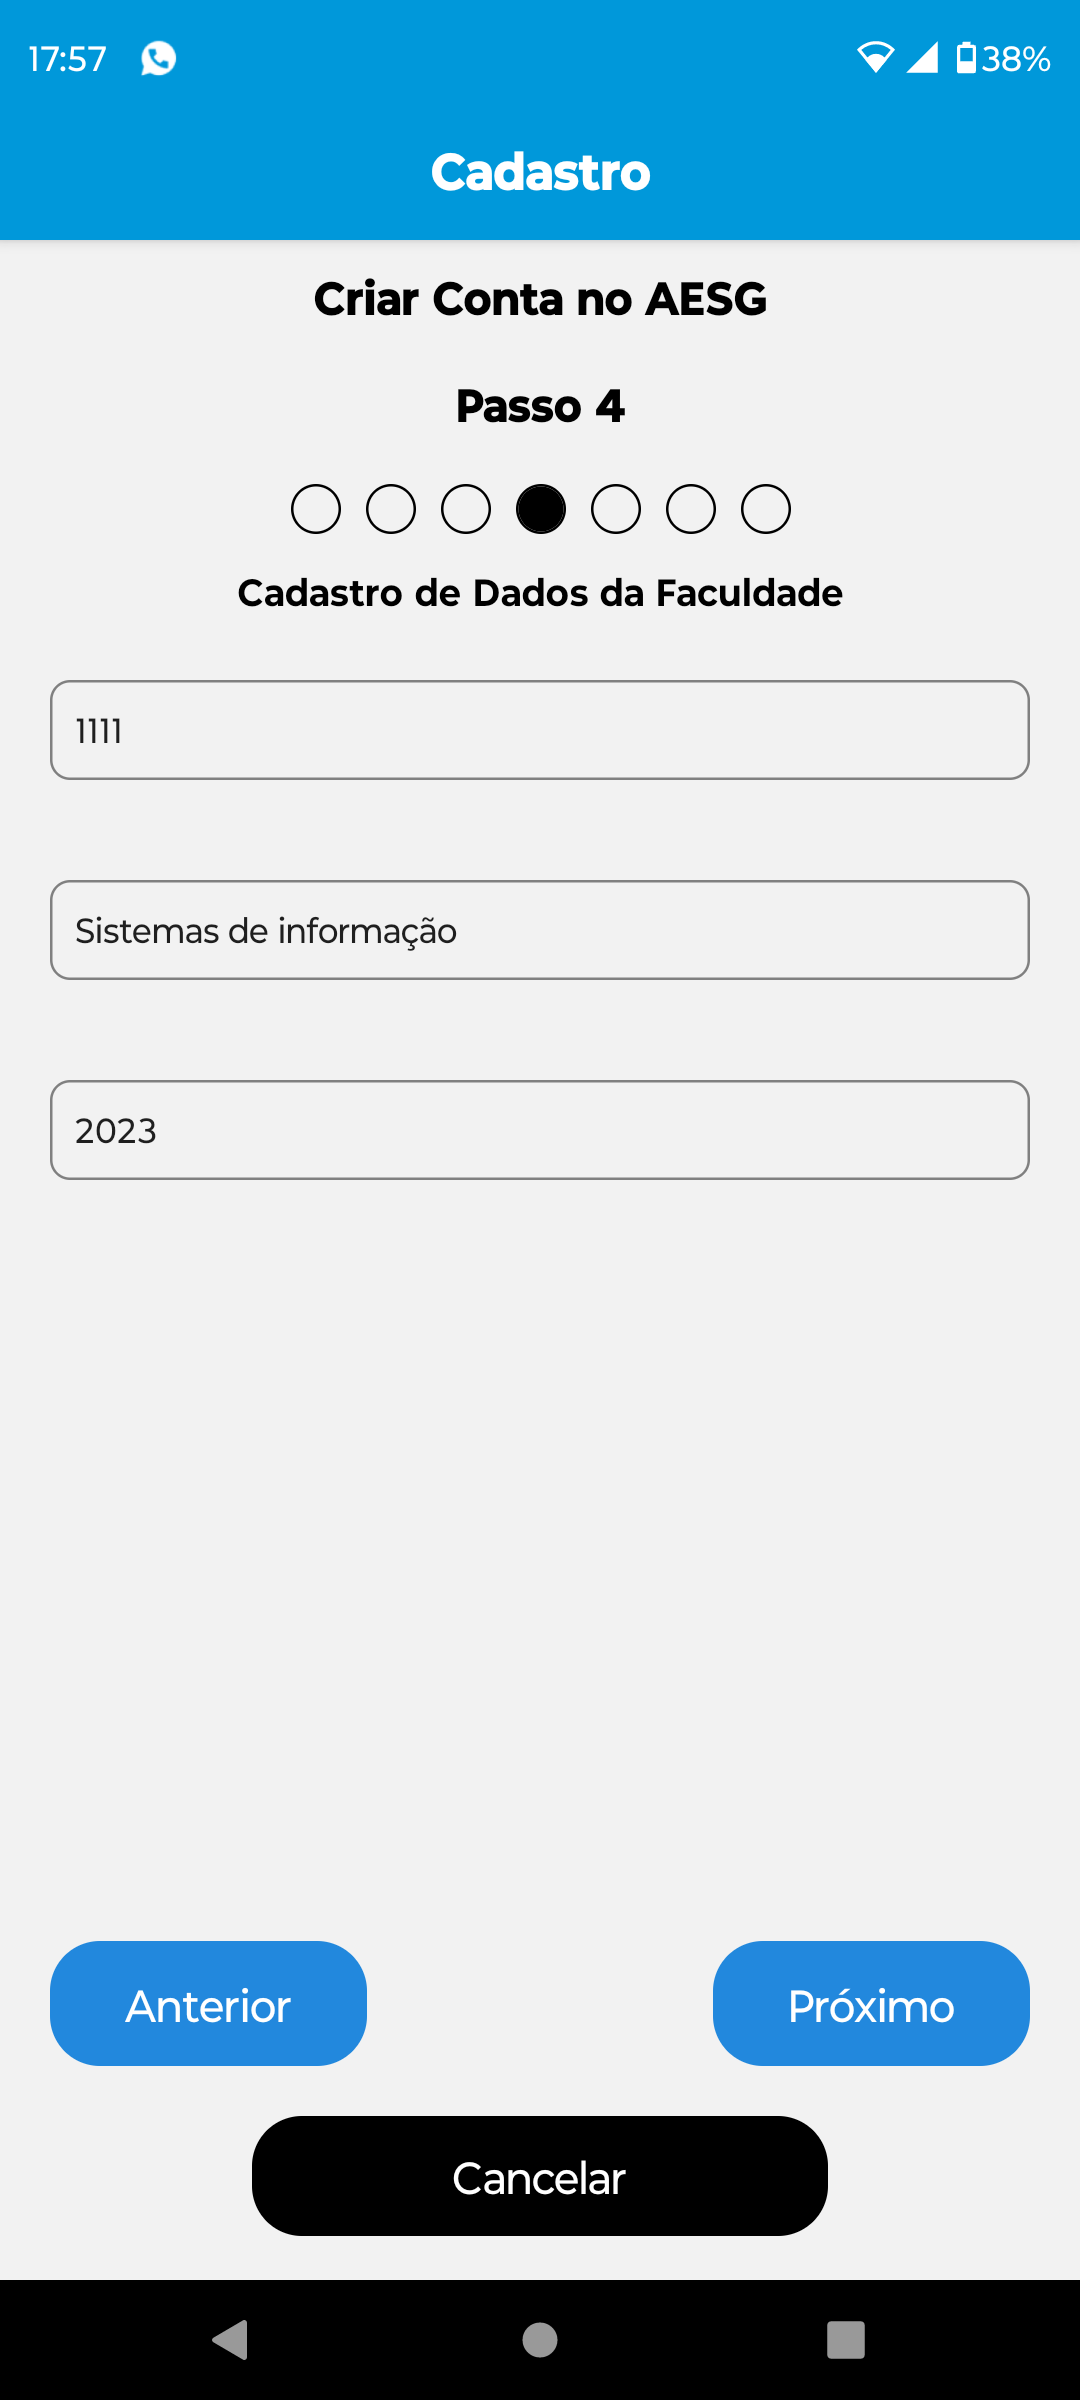
\includegraphics[width=0.8\linewidth]{Imagens/App Images User/AUCadastro4.png}
                    \caption[Imagem da Tela de Cadastro dos Dados da Faculdade Preenchido do Aplicativo AESG]{ 
                    Imagem da Tela de Cadastro dos Dados da Faculdade do Aplicativo AESG}
                    \label{fig:AppTelaCadastro4}
                    \legend{Fonte: O author}
                \end{minipage}
            \end{figure}
            \newpage
            Na tela do passo 5 o Usuário ira selecionar os horários que ira usar o ônibus tendo a opção dos turnos manhã, tarde e noite, na parte inferir da tela ele terá opções para voltar para o passo anterior ou prosseguir para o seguinte, a tela pode ser vista na Figura \ref{fig:AppTelaCadastro14} e Figura \ref{fig:AppTelaCadastro5}.
            \begin{figure}[!h]          
                \begin{minipage}{0.5\textwidth}
                    \centering
                    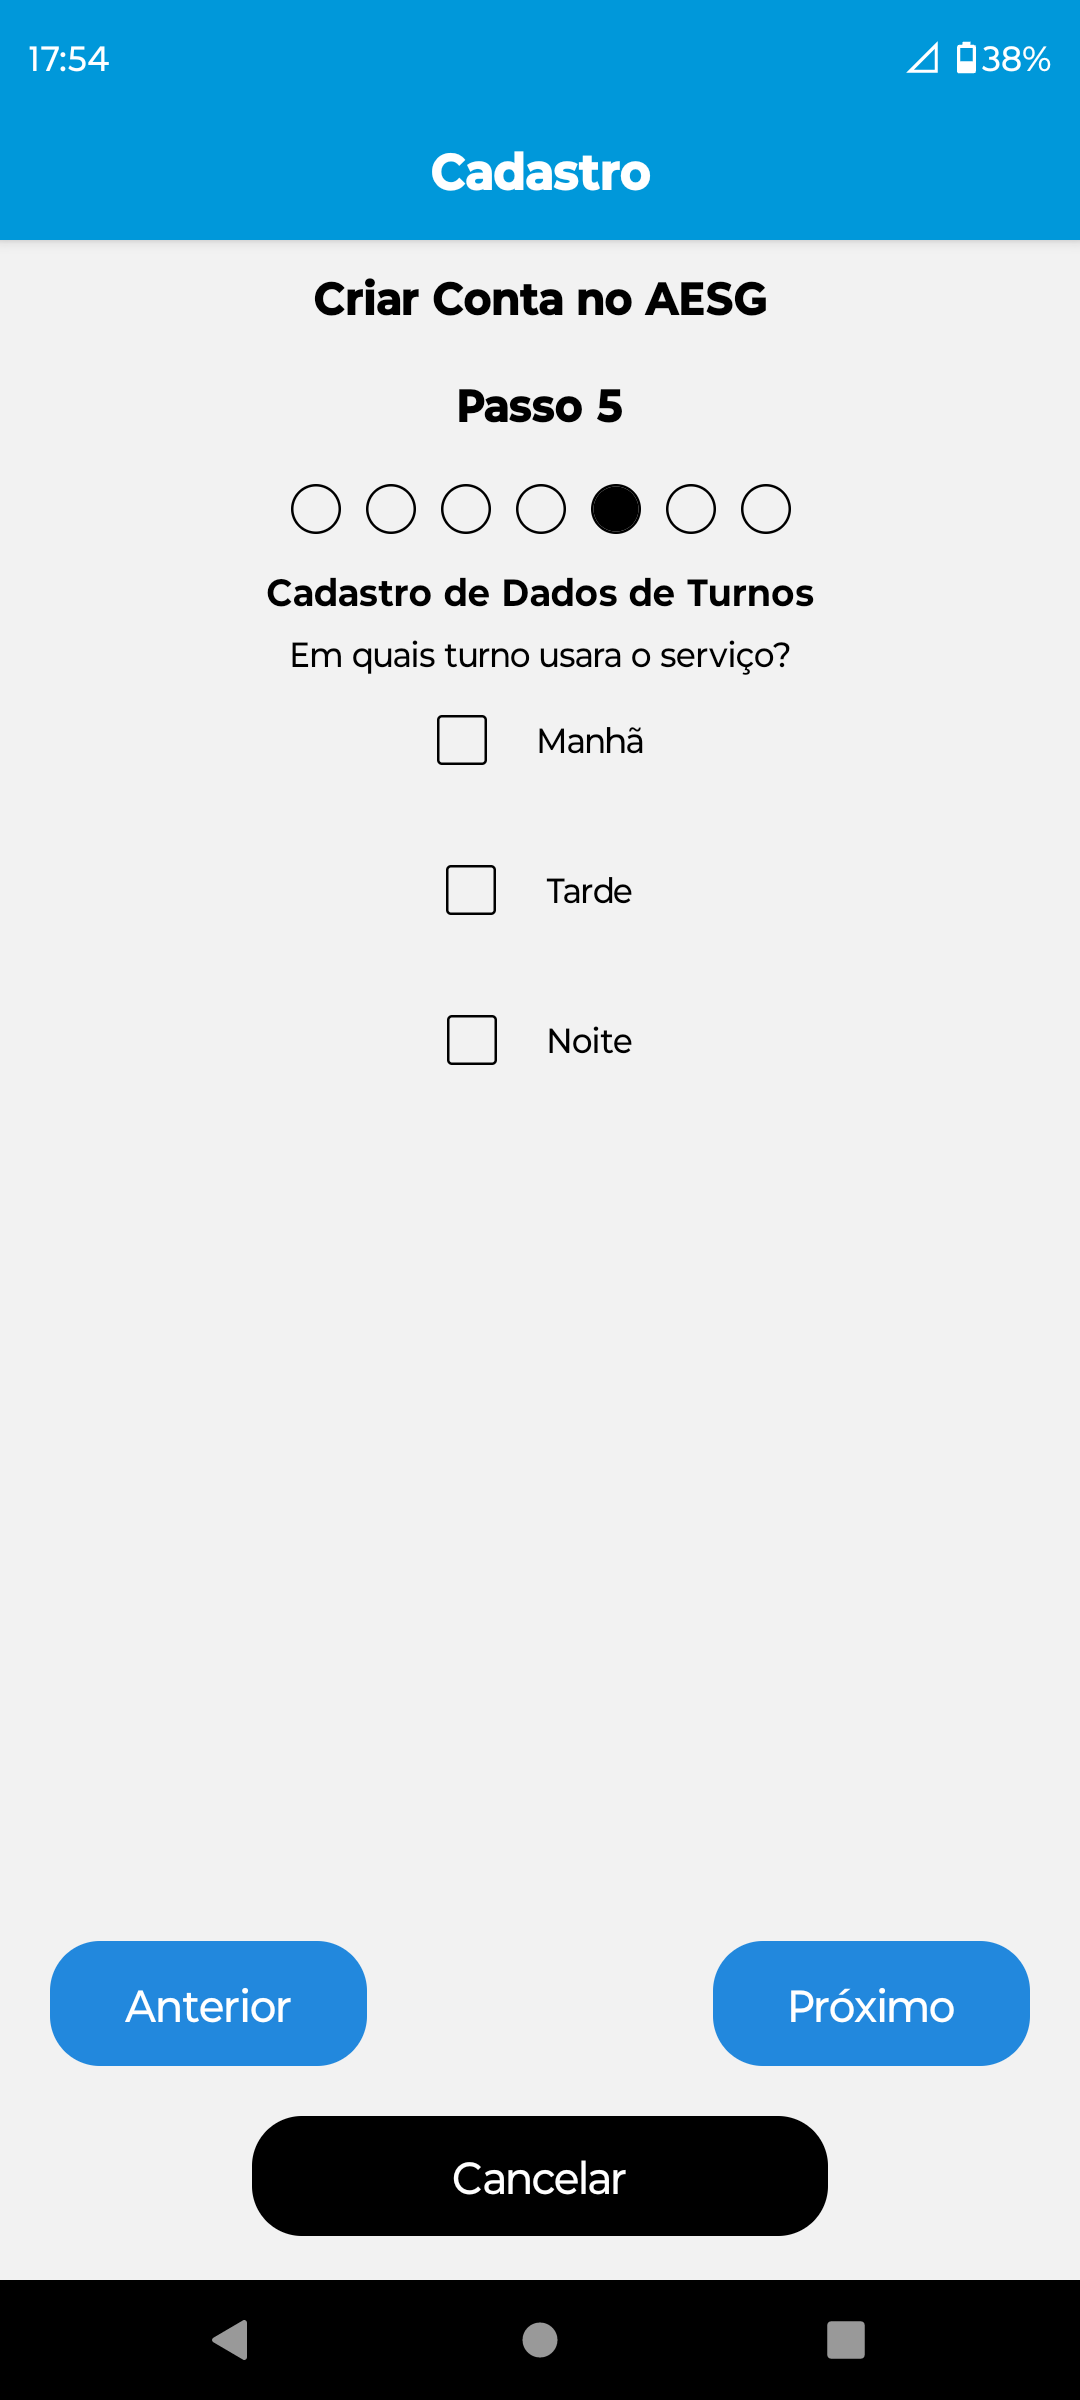
\includegraphics[width=0.8\linewidth]{Imagens/App Images User/AUCadastro14.png}
                    \caption[Imagem da Tela de Cadastro dos Dados de Turnos do Aplicativo AESG]{ 
                    Imagem da Tela de Cadastro dos Dados de Turnos do Aplicativo AESG}
                    \label{fig:AppTelaCadastro14}
                    \legend{Fonte: O author}
                \end{minipage}%
                \begin{minipage}{0.5\textwidth}
                    \centering
                    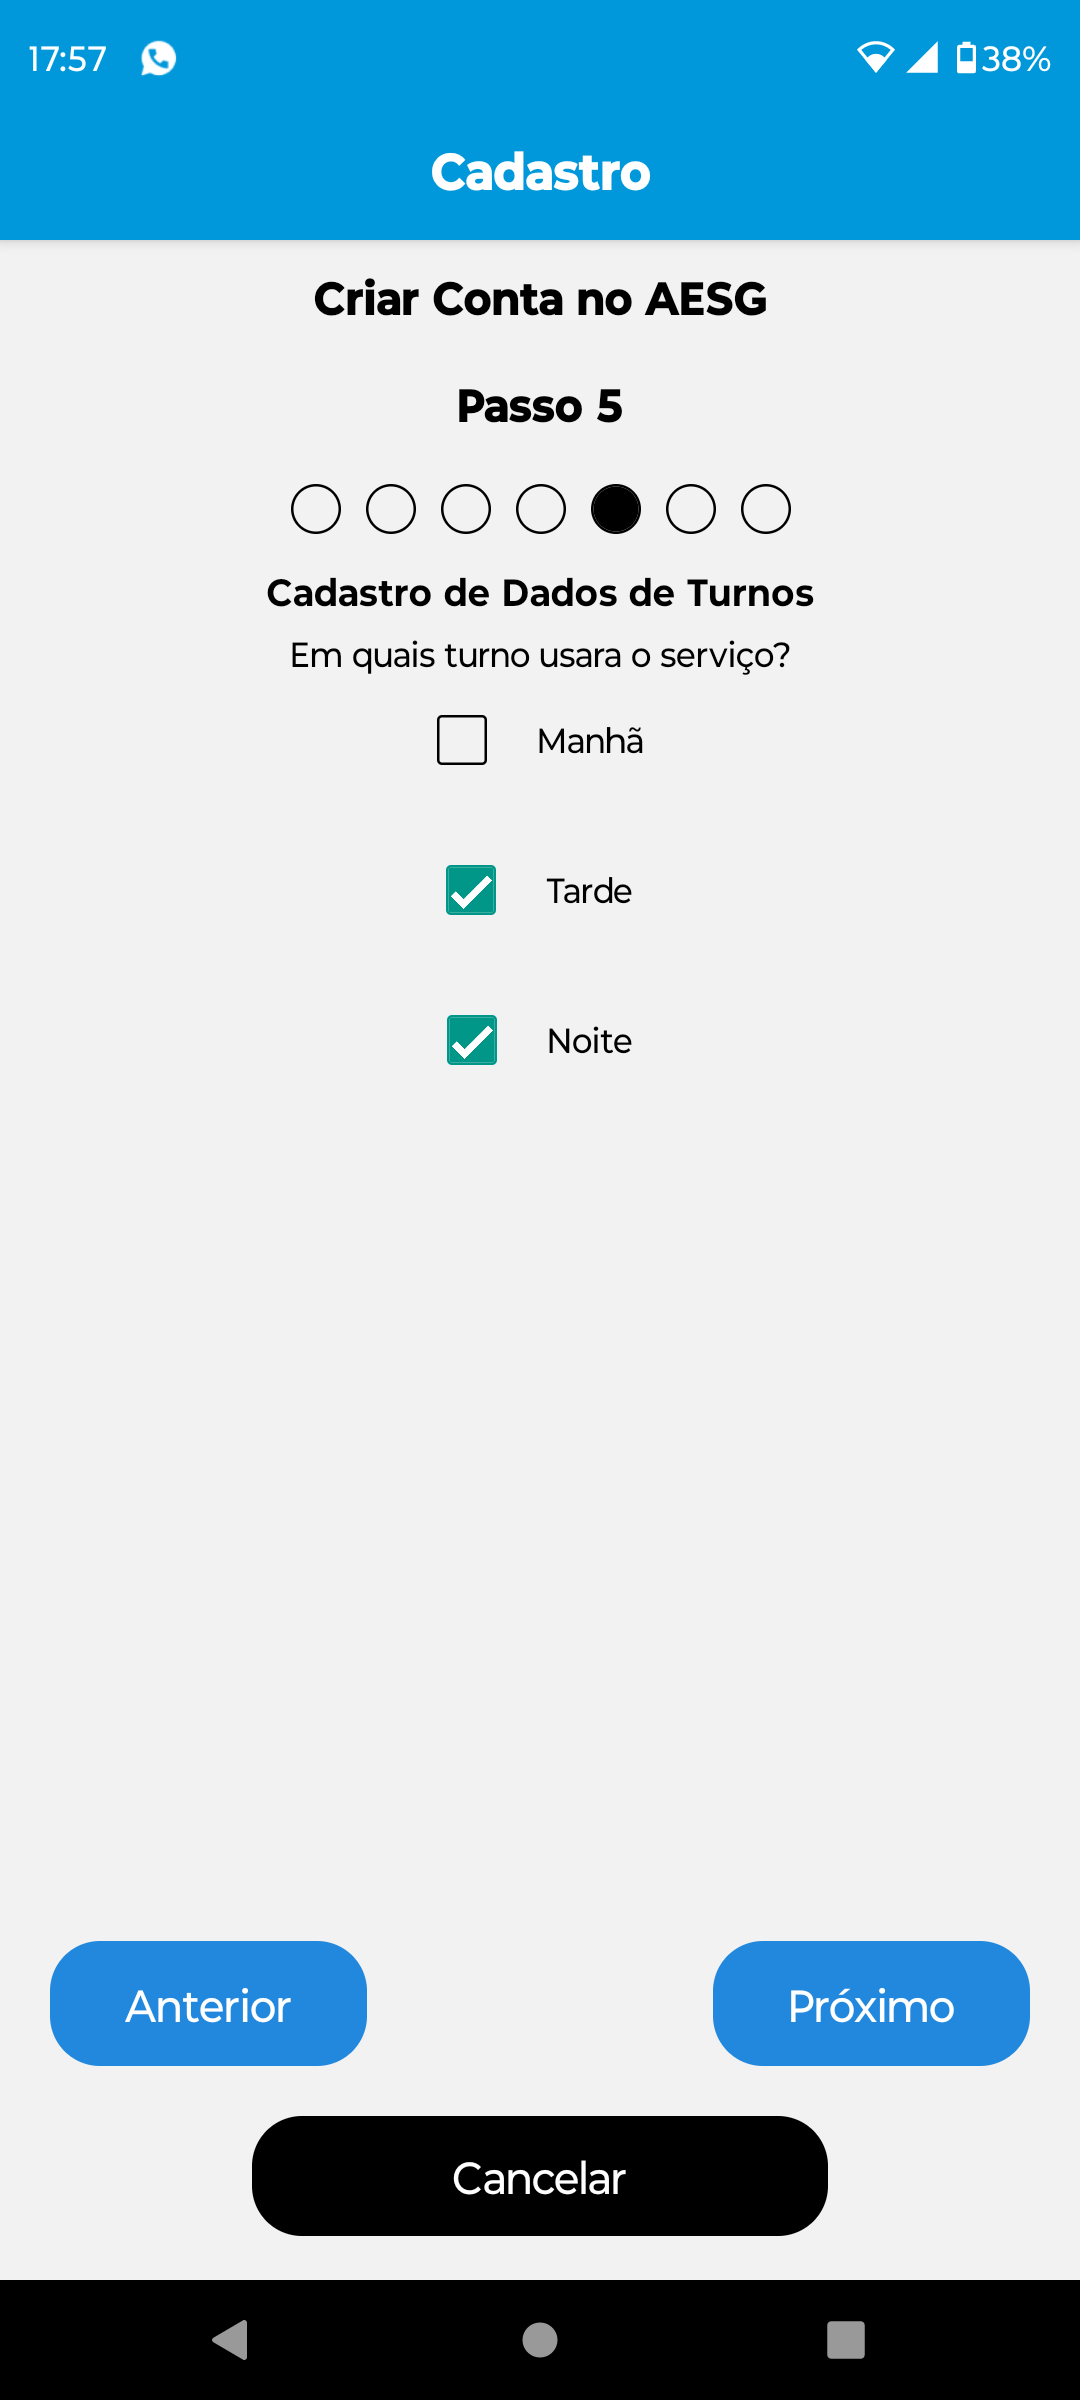
\includegraphics[width=0.8\linewidth]{Imagens/App Images User/AUCadastro5.png}
                    \caption[Imagem da Tela de Cadastro dos Dados de Turnos Preenchido do Aplicativo AESG]{ 
                    Imagem da Tela de Cadastro dos Dados  de Turnos do Aplicativo AESG}
                    \label{fig:AppTelaCadastro5}
                    \legend{Fonte: O author}
                \end{minipage}
            \end{figure}
            \newpage
            Na tela do passo 6 o Usuário ira selecionar uma foto de sua galeria para usar como foto de perfil no aplicativo, na parte inferir da tela ele terá opções para voltar para o passo anterior ou prosseguir para o seguinte, a tela pode ser vista na Figura \ref{fig:AppTelaCadastro15} e Figura \ref{fig:AppTelaCadastro6}.
            \begin{figure}[!h]          
                \begin{minipage}{0.5\textwidth}
                    \centering
                    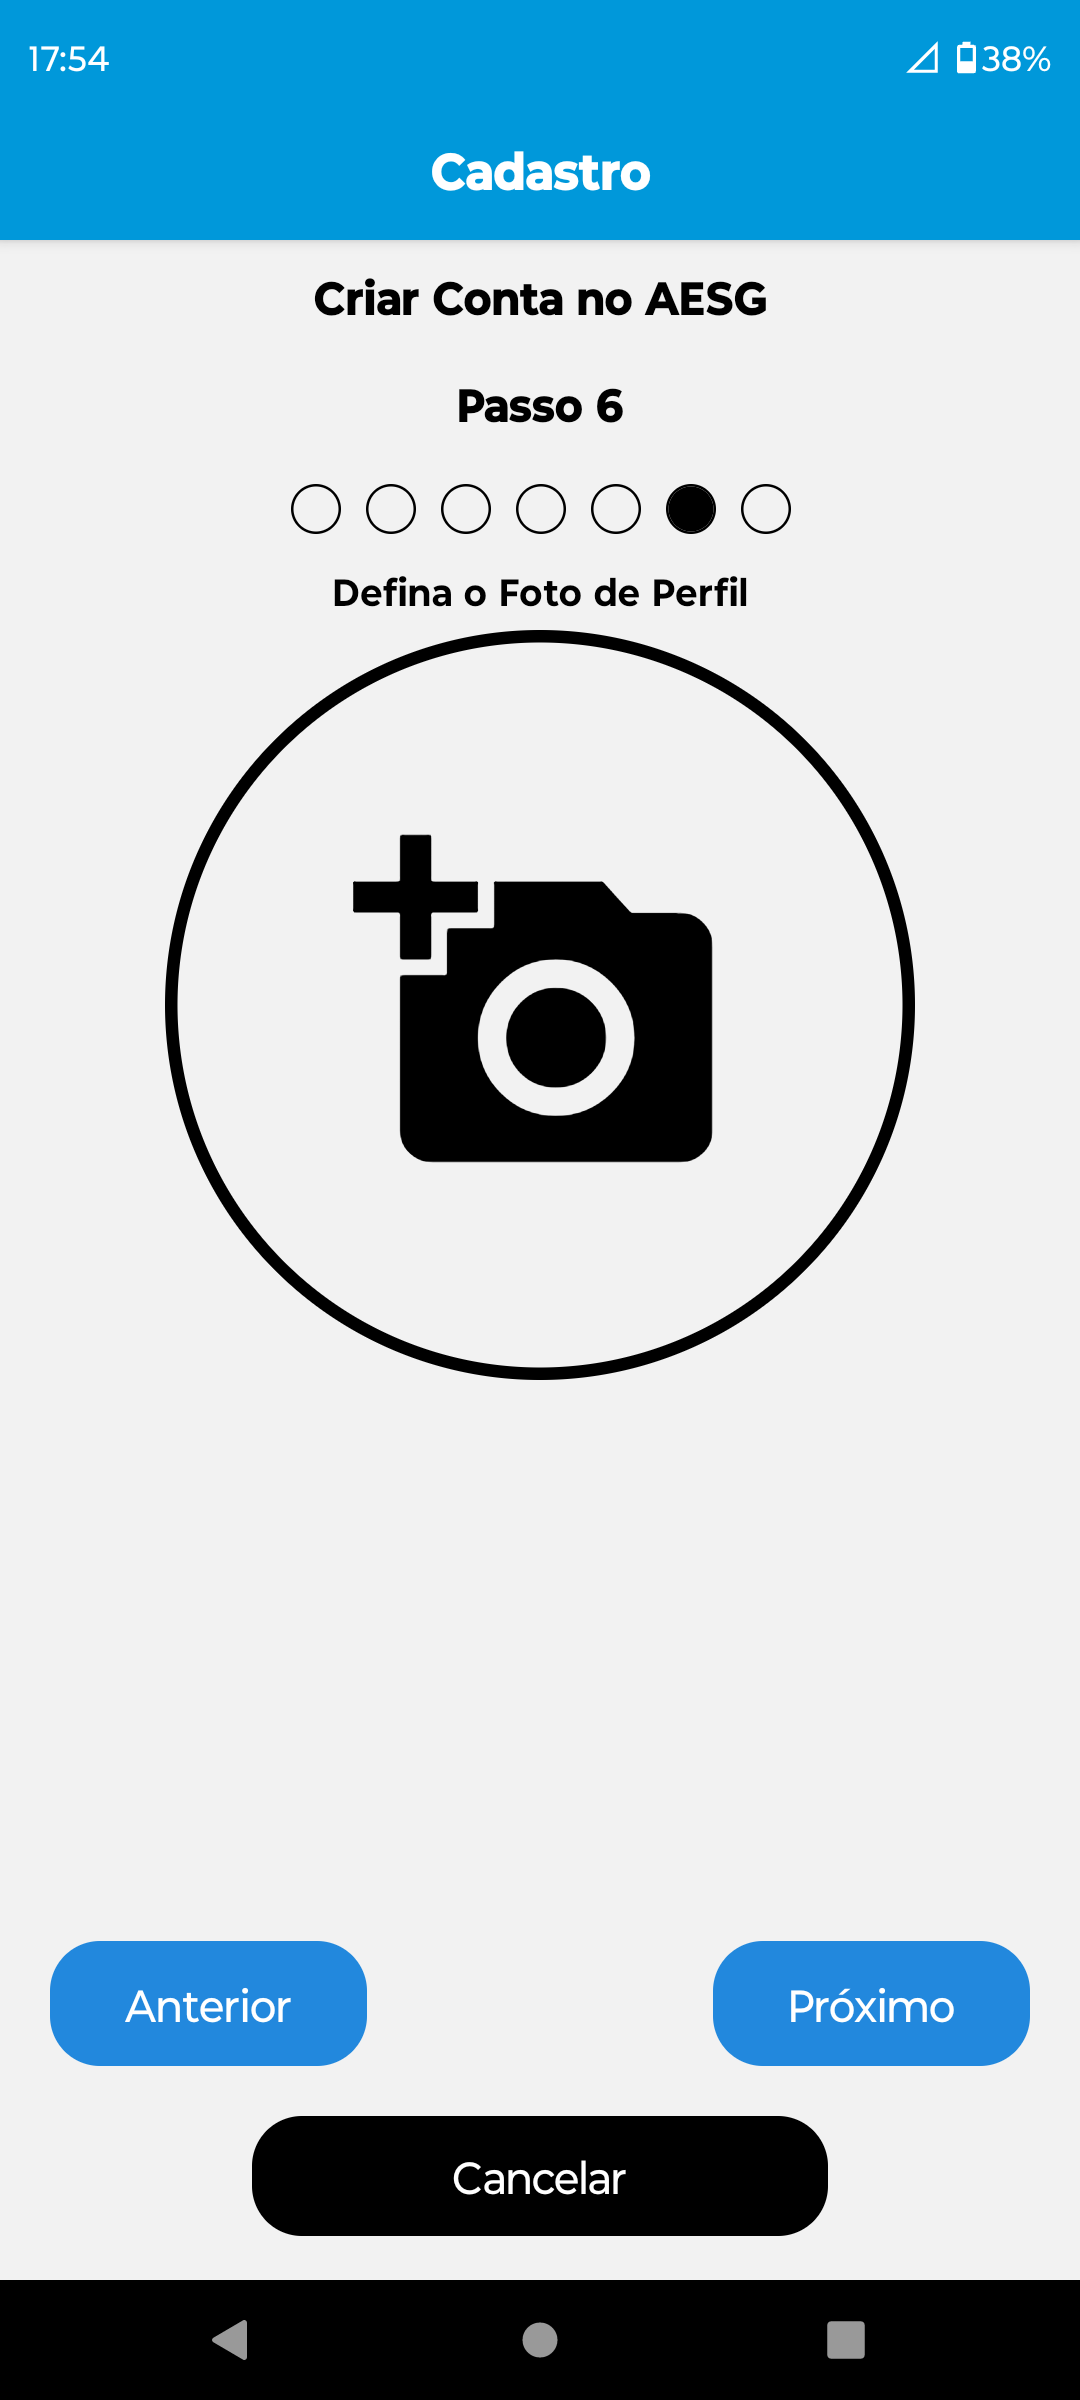
\includegraphics[width=0.8\linewidth]{Imagens/App Images User/AUCadastro15.png}
                    \caption[Imagem da Tela de Cadastro dos Dados de Foto de Perfil do Aplicativo AESG]{ 
                    Imagem da Tela de Cadastro dos Dados de Foto de Perfil  do Aplicativo AESG}
                    \label{fig:AppTelaCadastro15}
                    \legend{Fonte: O author}
                \end{minipage}%
                \begin{minipage}{0.5\textwidth}
                    \centering
                    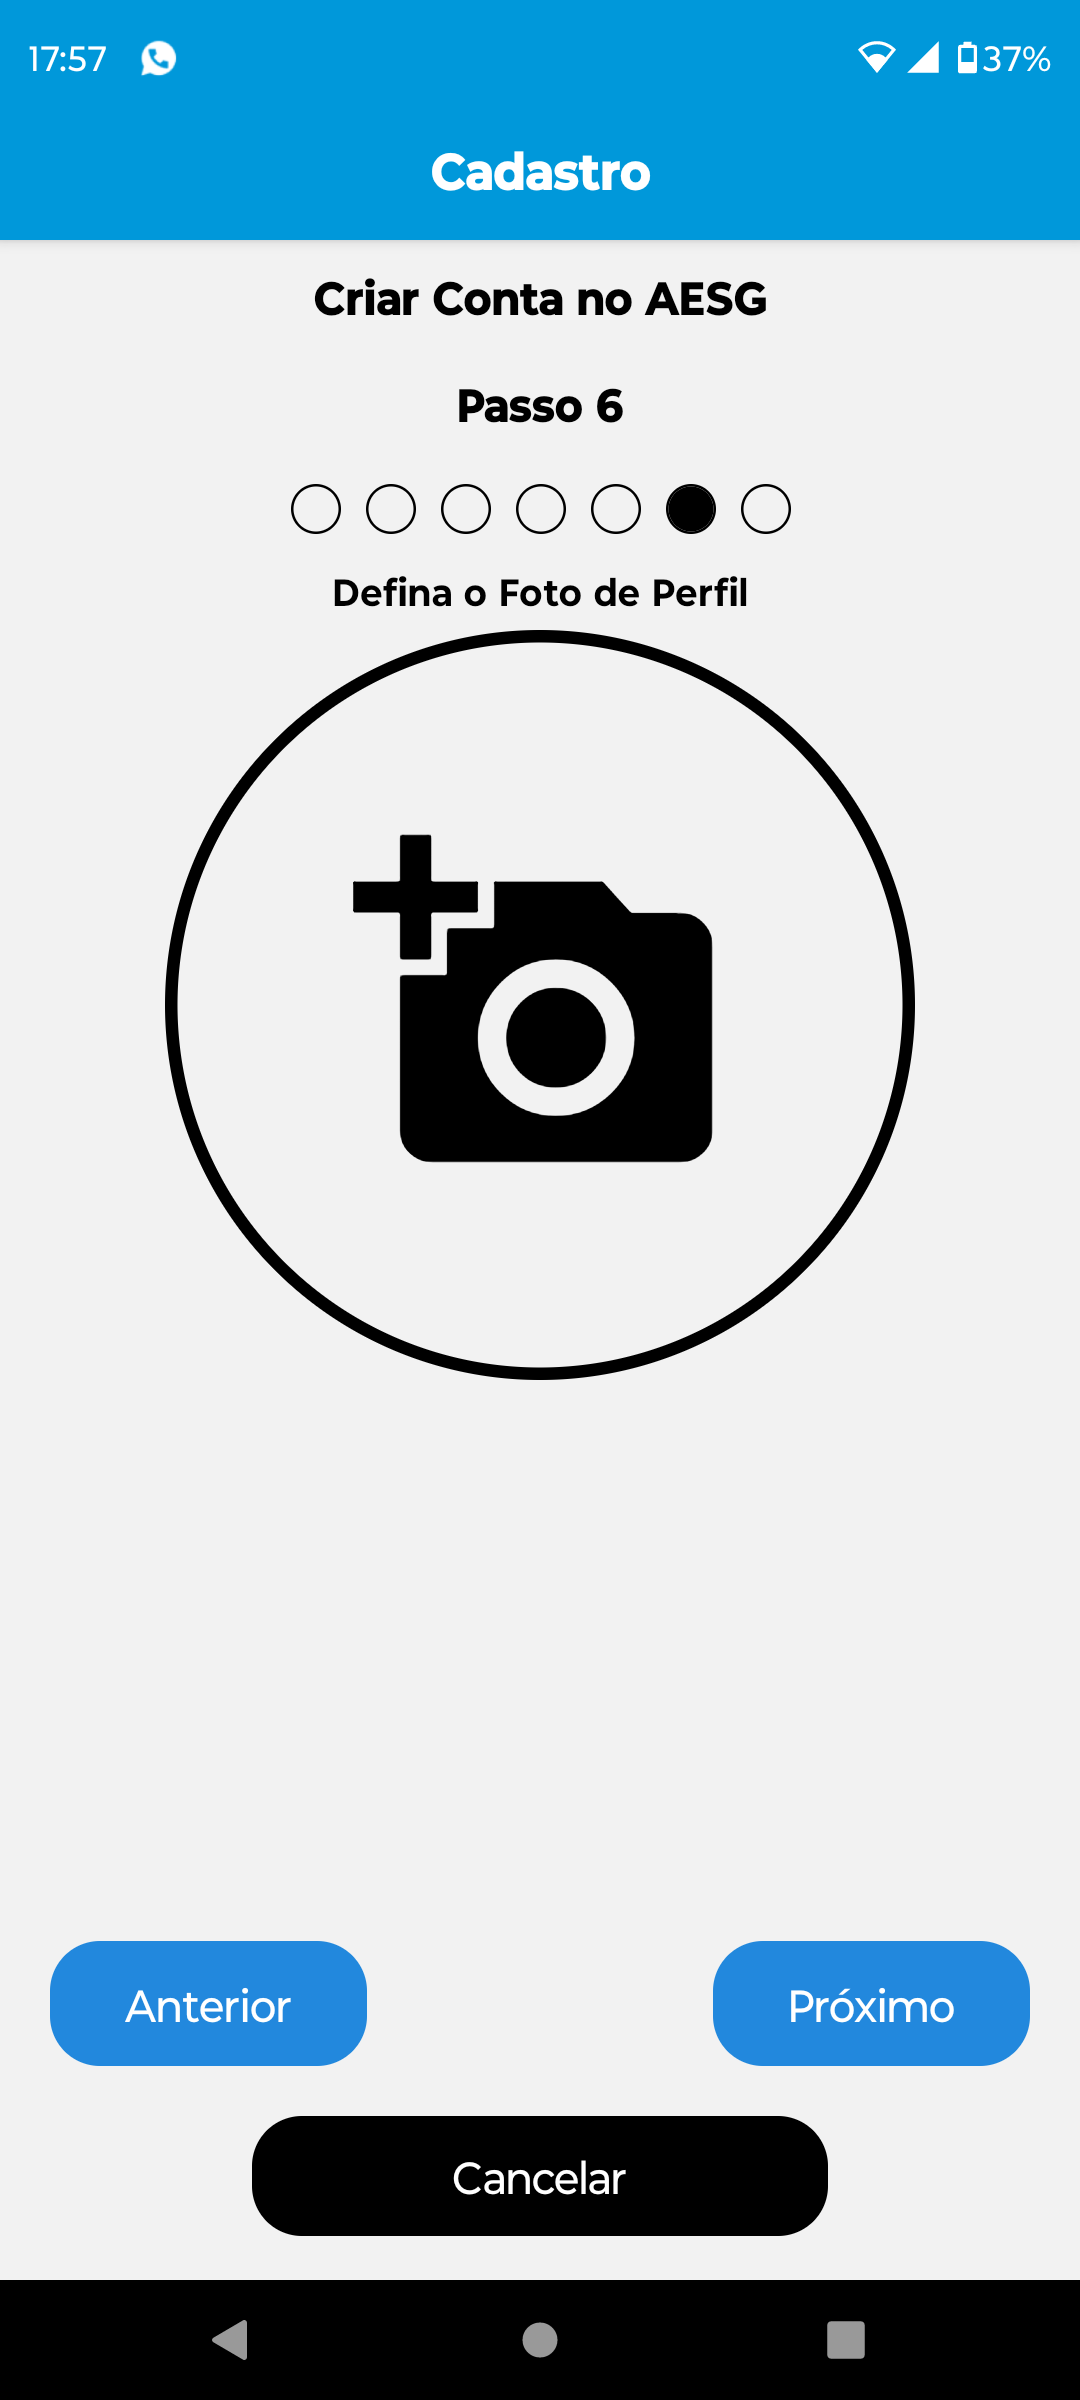
\includegraphics[width=0.8\linewidth]{Imagens/App Images User/AUCadastro6.png}
                    \caption[Imagem da Tela de Cadastro dos Dados de Foto de Perfil Preenchido do Aplicativo AESG]{ 
                    Imagem da Tela de Cadastro dos Dados  de Foto de Perfil do Aplicativo AESG}
                    \label{fig:AppTelaCadastro6}
                    \legend{Fonte: O author}
                \end{minipage}
            \end{figure}
            \newpage
            Na tela do passo 7 o Usuário poderá visualizar os dados que ele preencheu e validar antes de efetuar o cadastro, nesta tela ele vera todos os dados preenchidos dentro de suas categorias, na parte inferir da tela ele terá opções para voltar para o passo anterior ou prosseguir para o seguinte que no caso será  efetuação do cadastro, após o cadastro bem-sucedido o usuário será redirecionado para a aplicação em si, a tela pode ser vista na Figura \ref{fig:AppTelaCadastroConf1} e Figura \ref{fig:AppTelaCadastroConf2}.
            \begin{figure}[!h]          
                \begin{minipage}{0.5\textwidth}
                    \centering
                    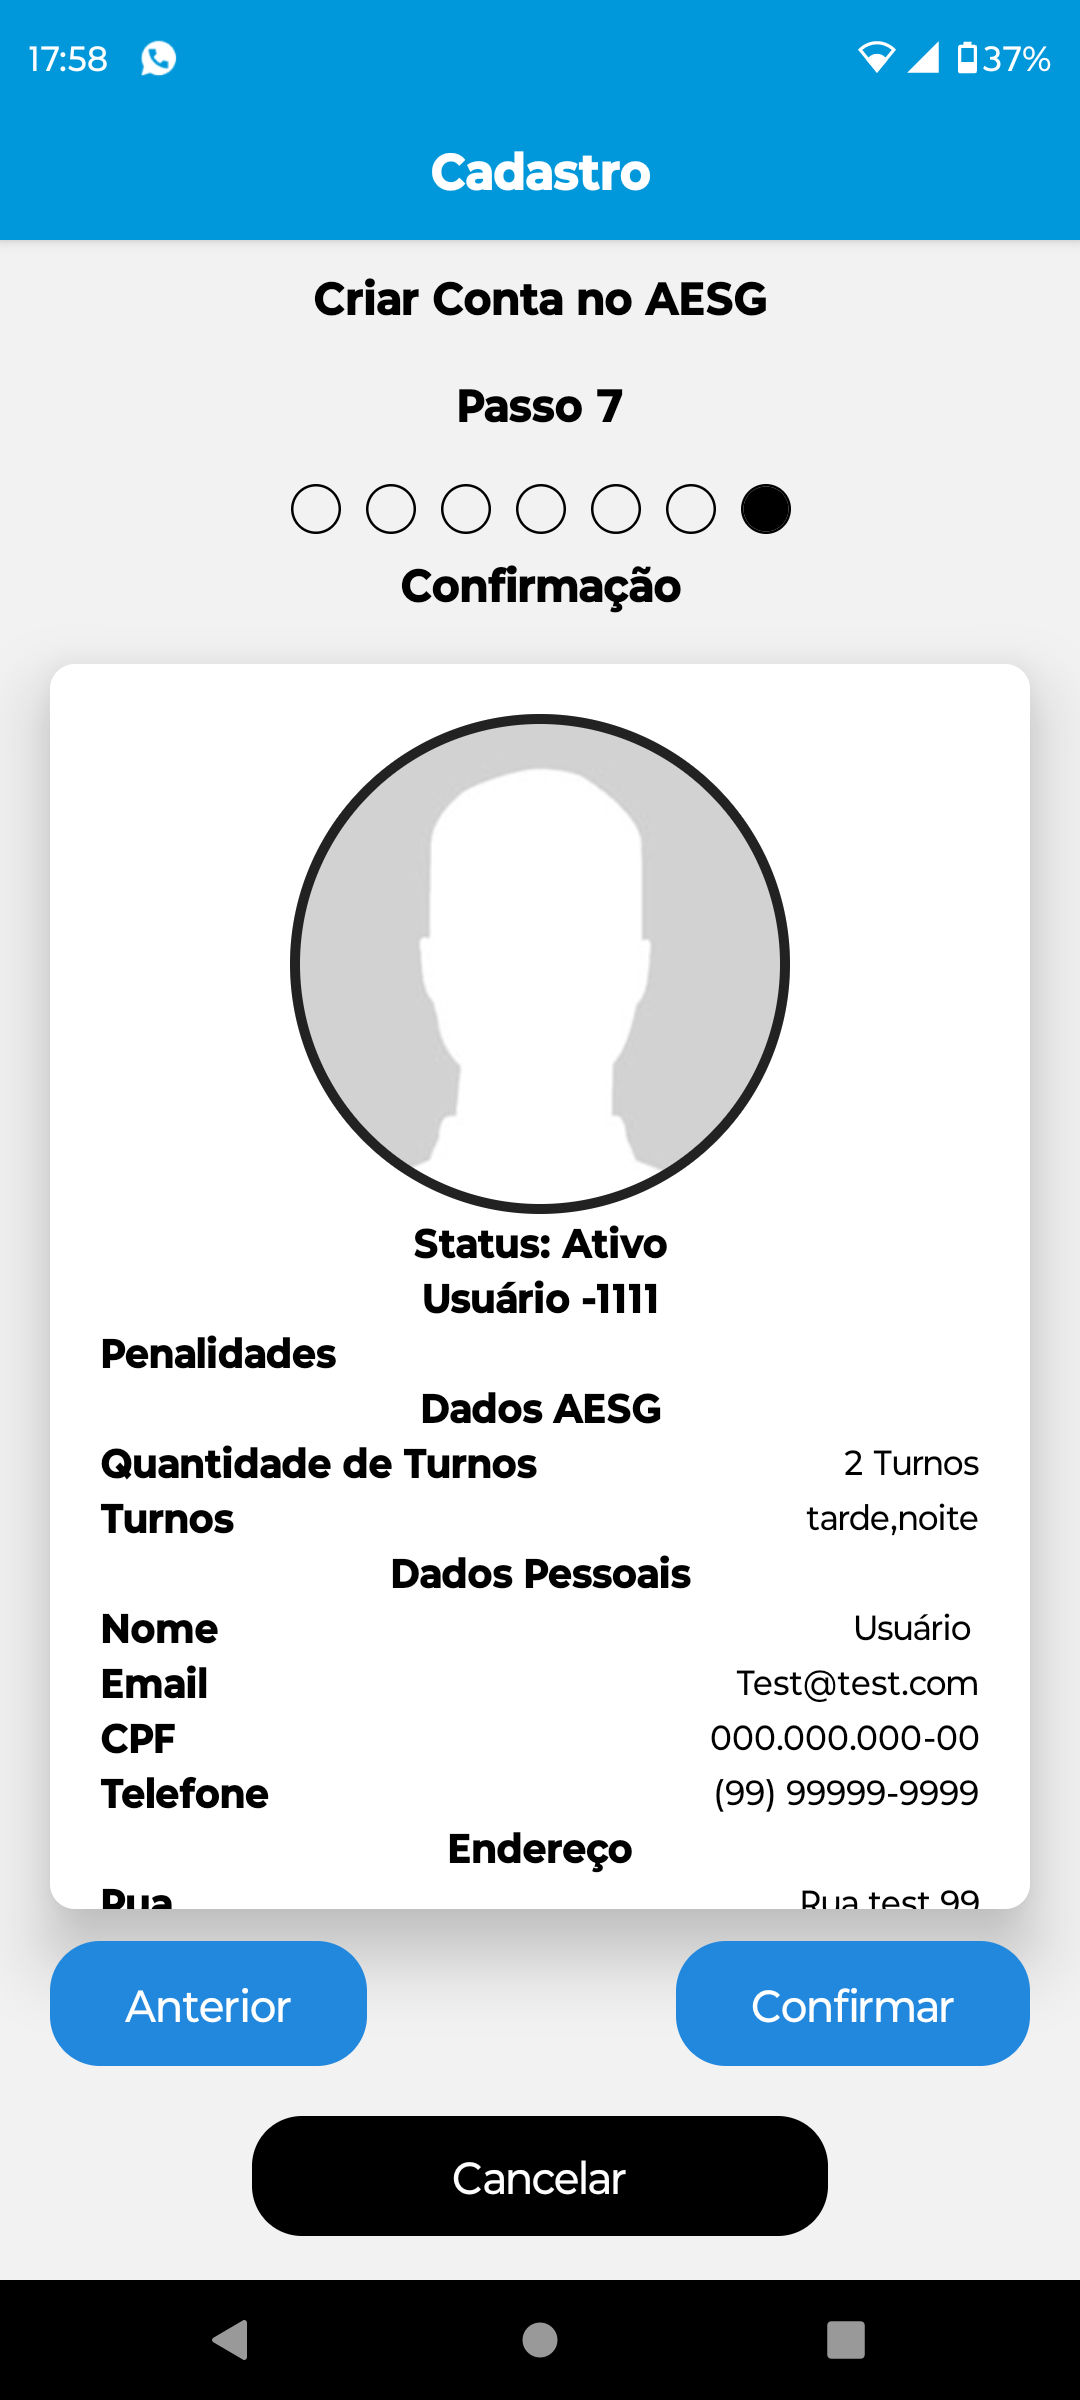
\includegraphics[width=0.8\linewidth]{Imagens/App Images User/AUCadastroConf1.png}
                    \caption[Imagem da Tela de Cadastro na Etapa de Confirmação dos Dados do Aplicativo AESG]{ 
                    Imagem da Tela de Cadastro na Etapa de Confirmação dos Dados  do Aplicativo AESG}
                    \label{fig:AppTelaCadastroConf1}
                    \legend{Fonte: O author}
                \end{minipage}%
                \begin{minipage}{0.5\textwidth}
                    \centering
                    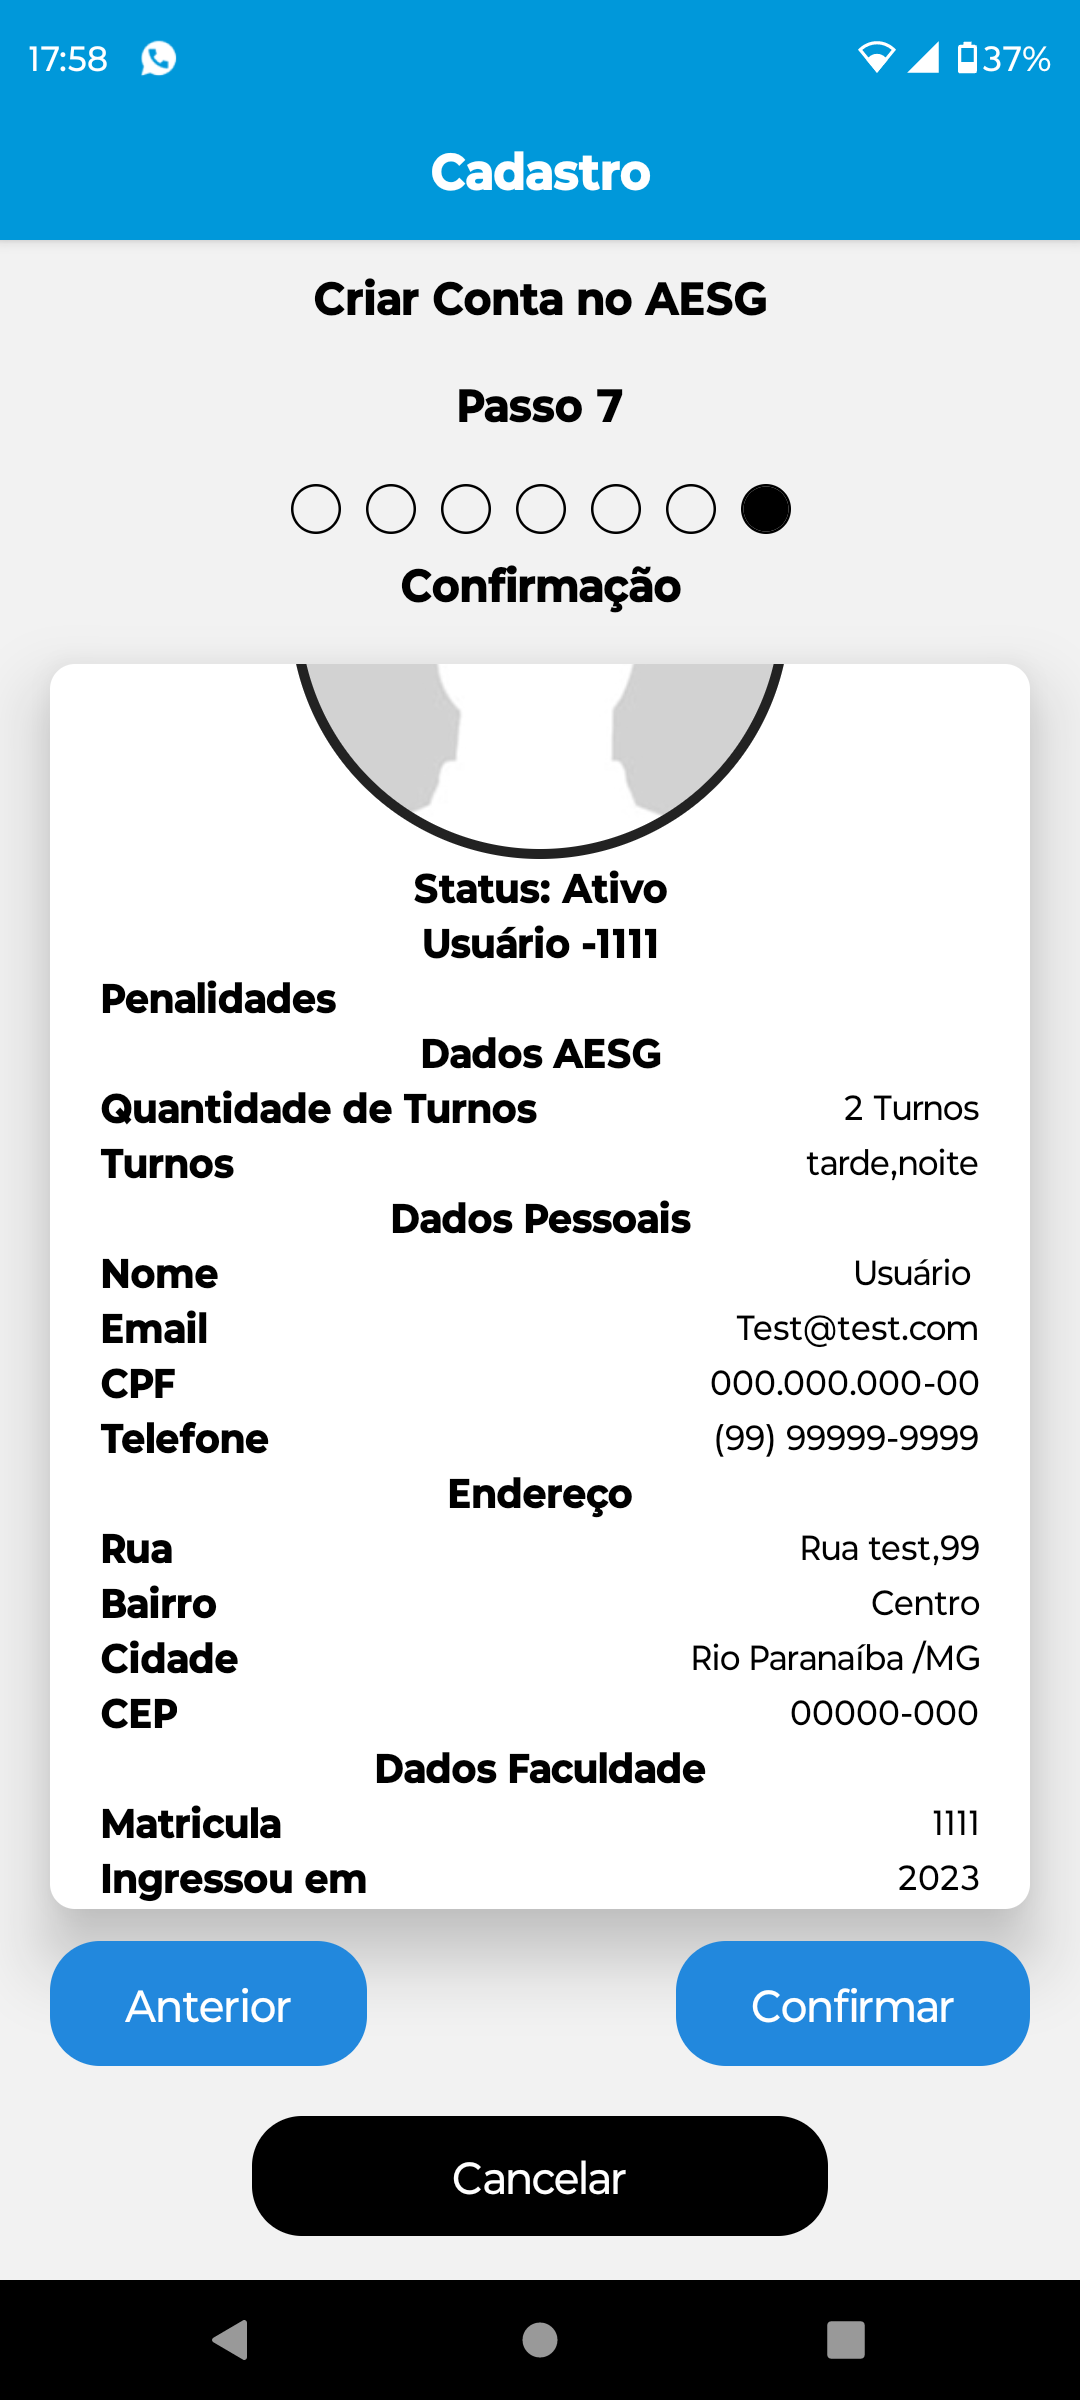
\includegraphics[width=0.8\linewidth]{Imagens/App Images User/AUCadastroConf2.png}
                    \caption[Imagem da Tela de Cadastro na Etapa de Confirmação dos Dados do Aplicativo AESG]{ 
                    Imagem da Tela de Cadastro na Etapa de Confirmação dos Dados do Aplicativo AESG}
                    \label{fig:AppTelaCadastroConf2}
                    \legend{Fonte: O author}
                \end{minipage}
            \end{figure}
        \newpage
        \subsection{Tela Home}
            Após efetuar o login ou cadastro o usuário será redirecionado para a tela Home ao ele tera se nome, matricula e foto de perfil exibidos na parte superior da página, logo abaixo disso se encontra a área de avisos aonde aviso da comissão poderão ser exibidos, e abaixo disso existe a área de listagem de pagamentos pendentes aonde o usuário visualizara resumidamente apenas pagamentos pendentes, podem clicar no pagamento para visualizar mais detalhes ou até acessar as opções de pagamentos, na parte inferior desta tela ele tem a \textit{TabBar} que permite ao usuário navegar entre as principais telas da aplicação, esta tela pode ser vista na Figura \ref{fig:AppTelaHome}.

            \begin{figure}[!h]
                \begin{center}
                \centering
                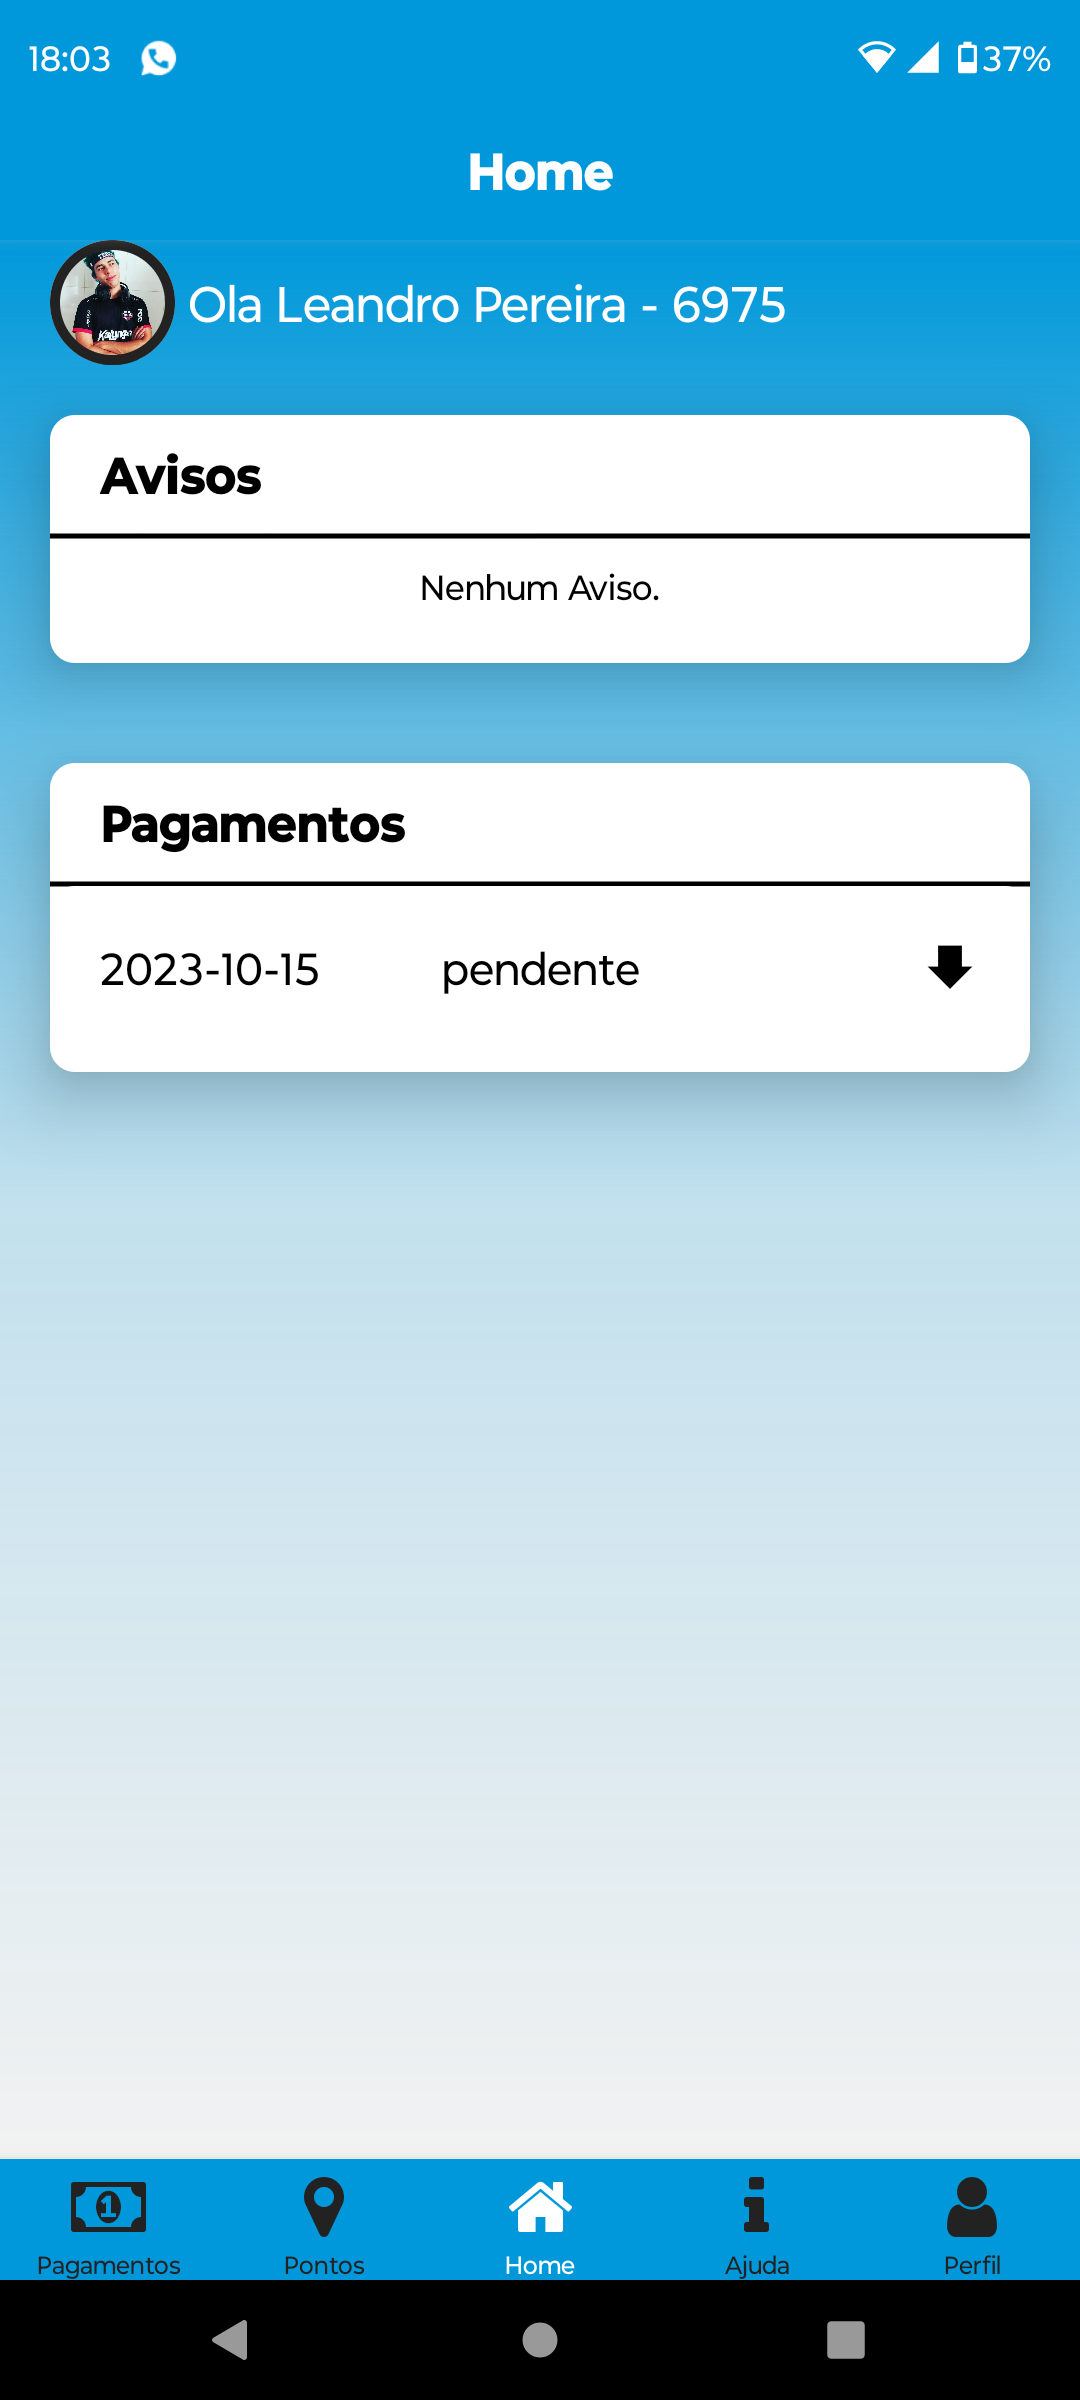
\includegraphics[width=0.4\linewidth]{Imagens/App Images User/AUHome.png}
                \end{center}
                \caption[Imagem da Tela Home do Aplicativo AESG]{ 
                Imagem da Tela Home do Aplicativo AESG}
                \label{fig:AppTelaHome}
                \legend{Fonte: O author}
            \end{figure}

        \newpage
        \subsection{Tela de Perfil}
            A partir do menu na parte inferior o usuário poderá acessar a tela de perfil, aonde ele poderá visualizar todos os dados de seu cadastro e fazer alterações, a pagina apresente a foto de perfil na parte superior seguida dos dados do usuário, na parte inferior da tele existem dois botões editar e sair, aonde em editar o usuário tem acesso a modificar seus dados de cadastro, enquanto no botão sair ele poderá sair de sua conta e retornar a tela inicial da aplicação, aonde poderá efetuar um novo login ou cadastro, esta tela pode ser vista na Figura \ref{fig:AppTelaPerfil}.
    
            \begin{figure}[!h]
                \begin{center}
                \centering
                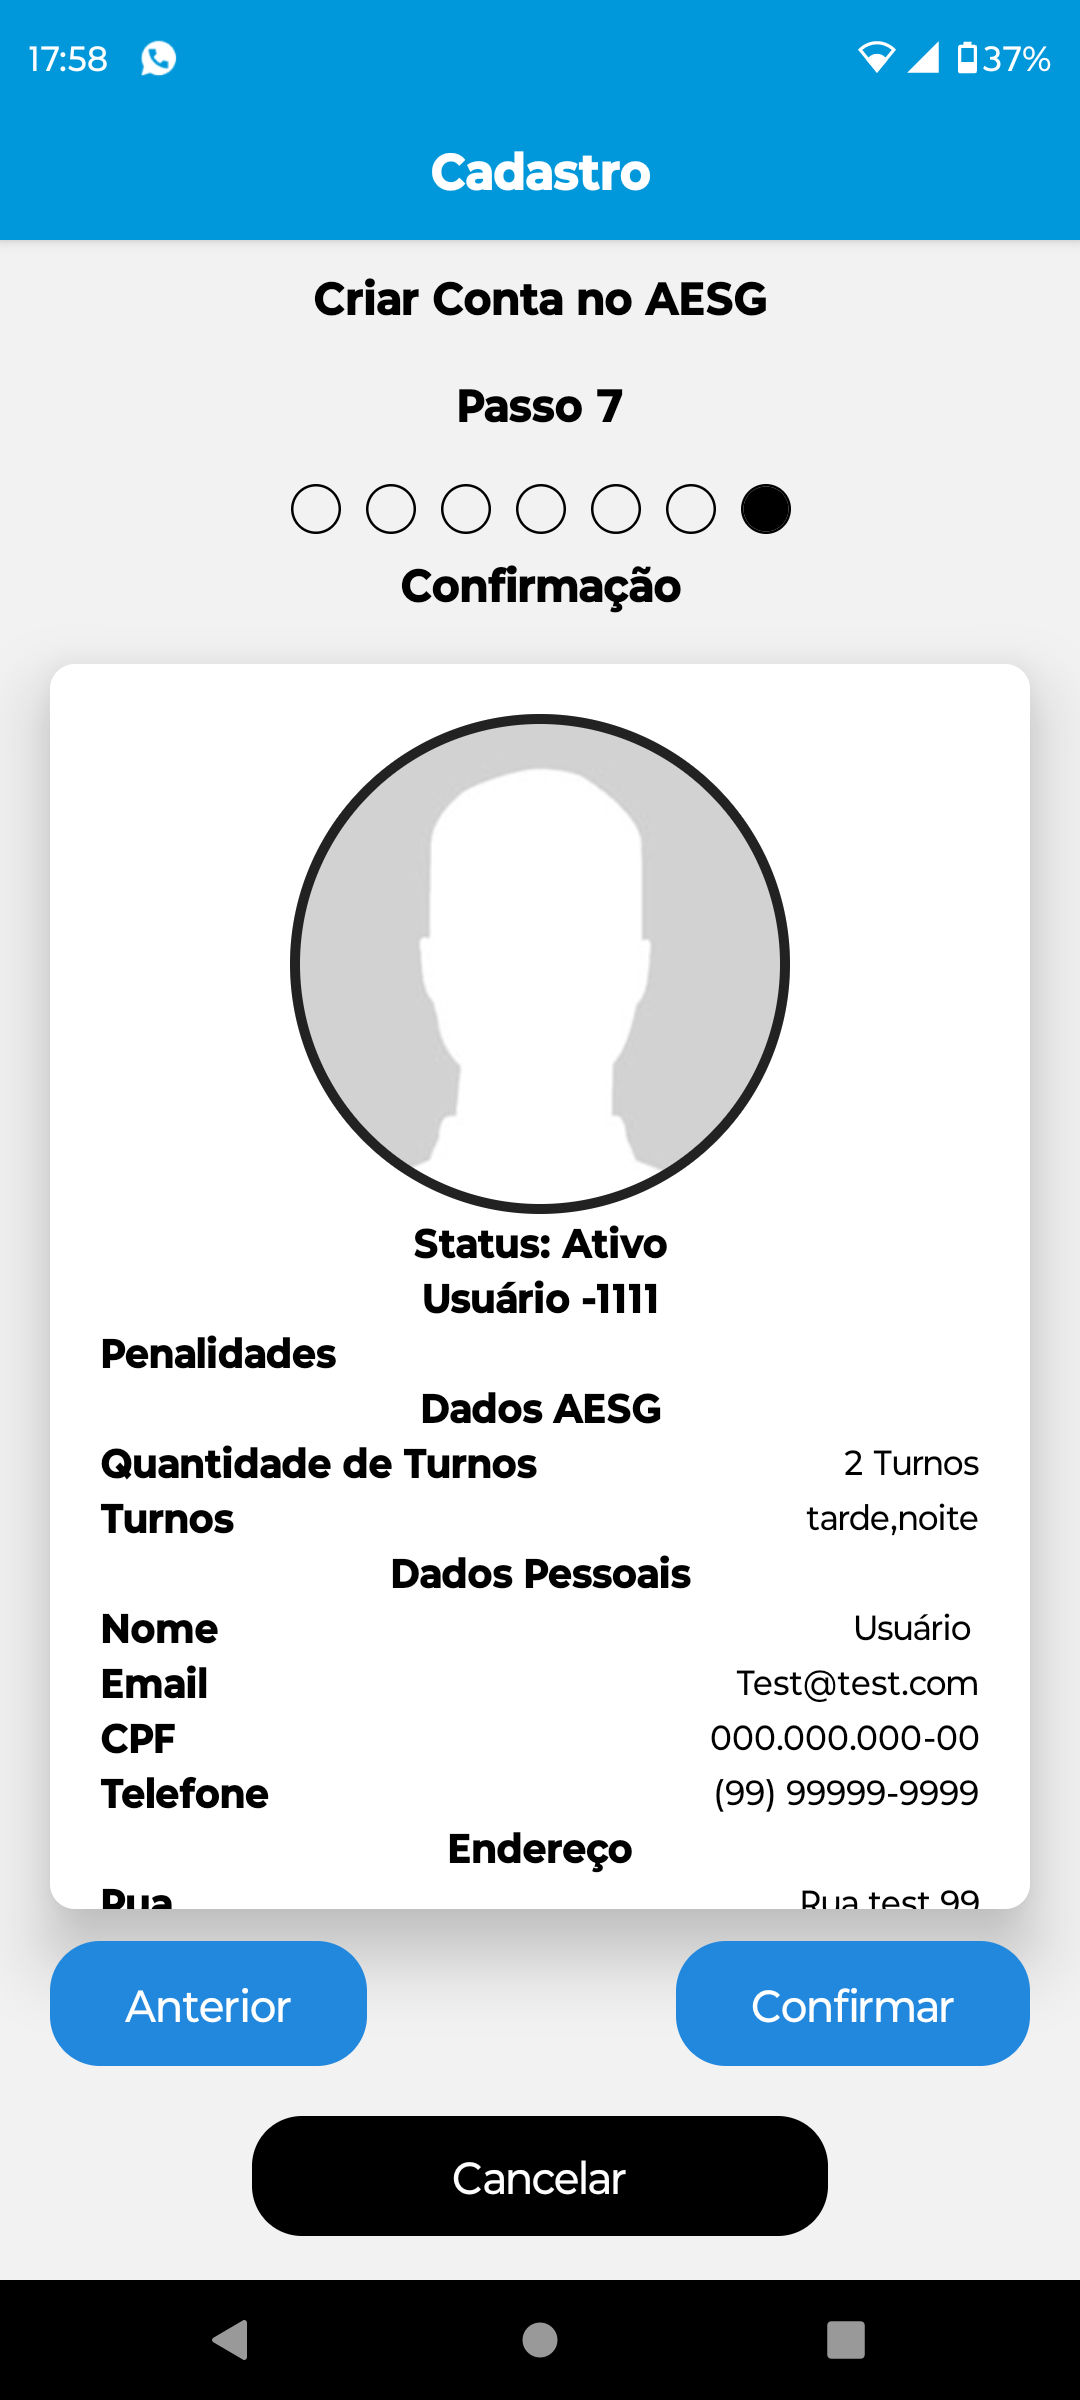
\includegraphics[width=0.4\linewidth]{Imagens/App Images User/AUCadastroConf1.png}
                \end{center}
                \caption[Imagem da Tela Perfil do Aplicativo AESG]{ 
                Imagem da Tela Perfil do Aplicativo AESG}
                \label{fig:AppTelaPerfil}
                \legend{Fonte: O author}
            \end{figure}

        \subsection{Tela de Ajuda}
            A partir do menu na parte inferior o usuário poderá acessar a tela de ajuda, aonde ele poderá visualizar um FAQ onde estão respostas para perguntas comuns do usuário de esclarecimentos sobre o funcionamentos dos processos da associação, são aprestadas na tela perguntas bem objetivas e ao clicar nelas o usuário terá acesso a um testo rápido respondendo aquela pergunta, esta tela pode ser vista na Figura \ref{fig:AppTelaAjuda} e Figura \ref{fig:AppTelaAjuda2}.

            \begin{figure}[!h]          
                \begin{minipage}{0.5\textwidth}
                    \centering
                    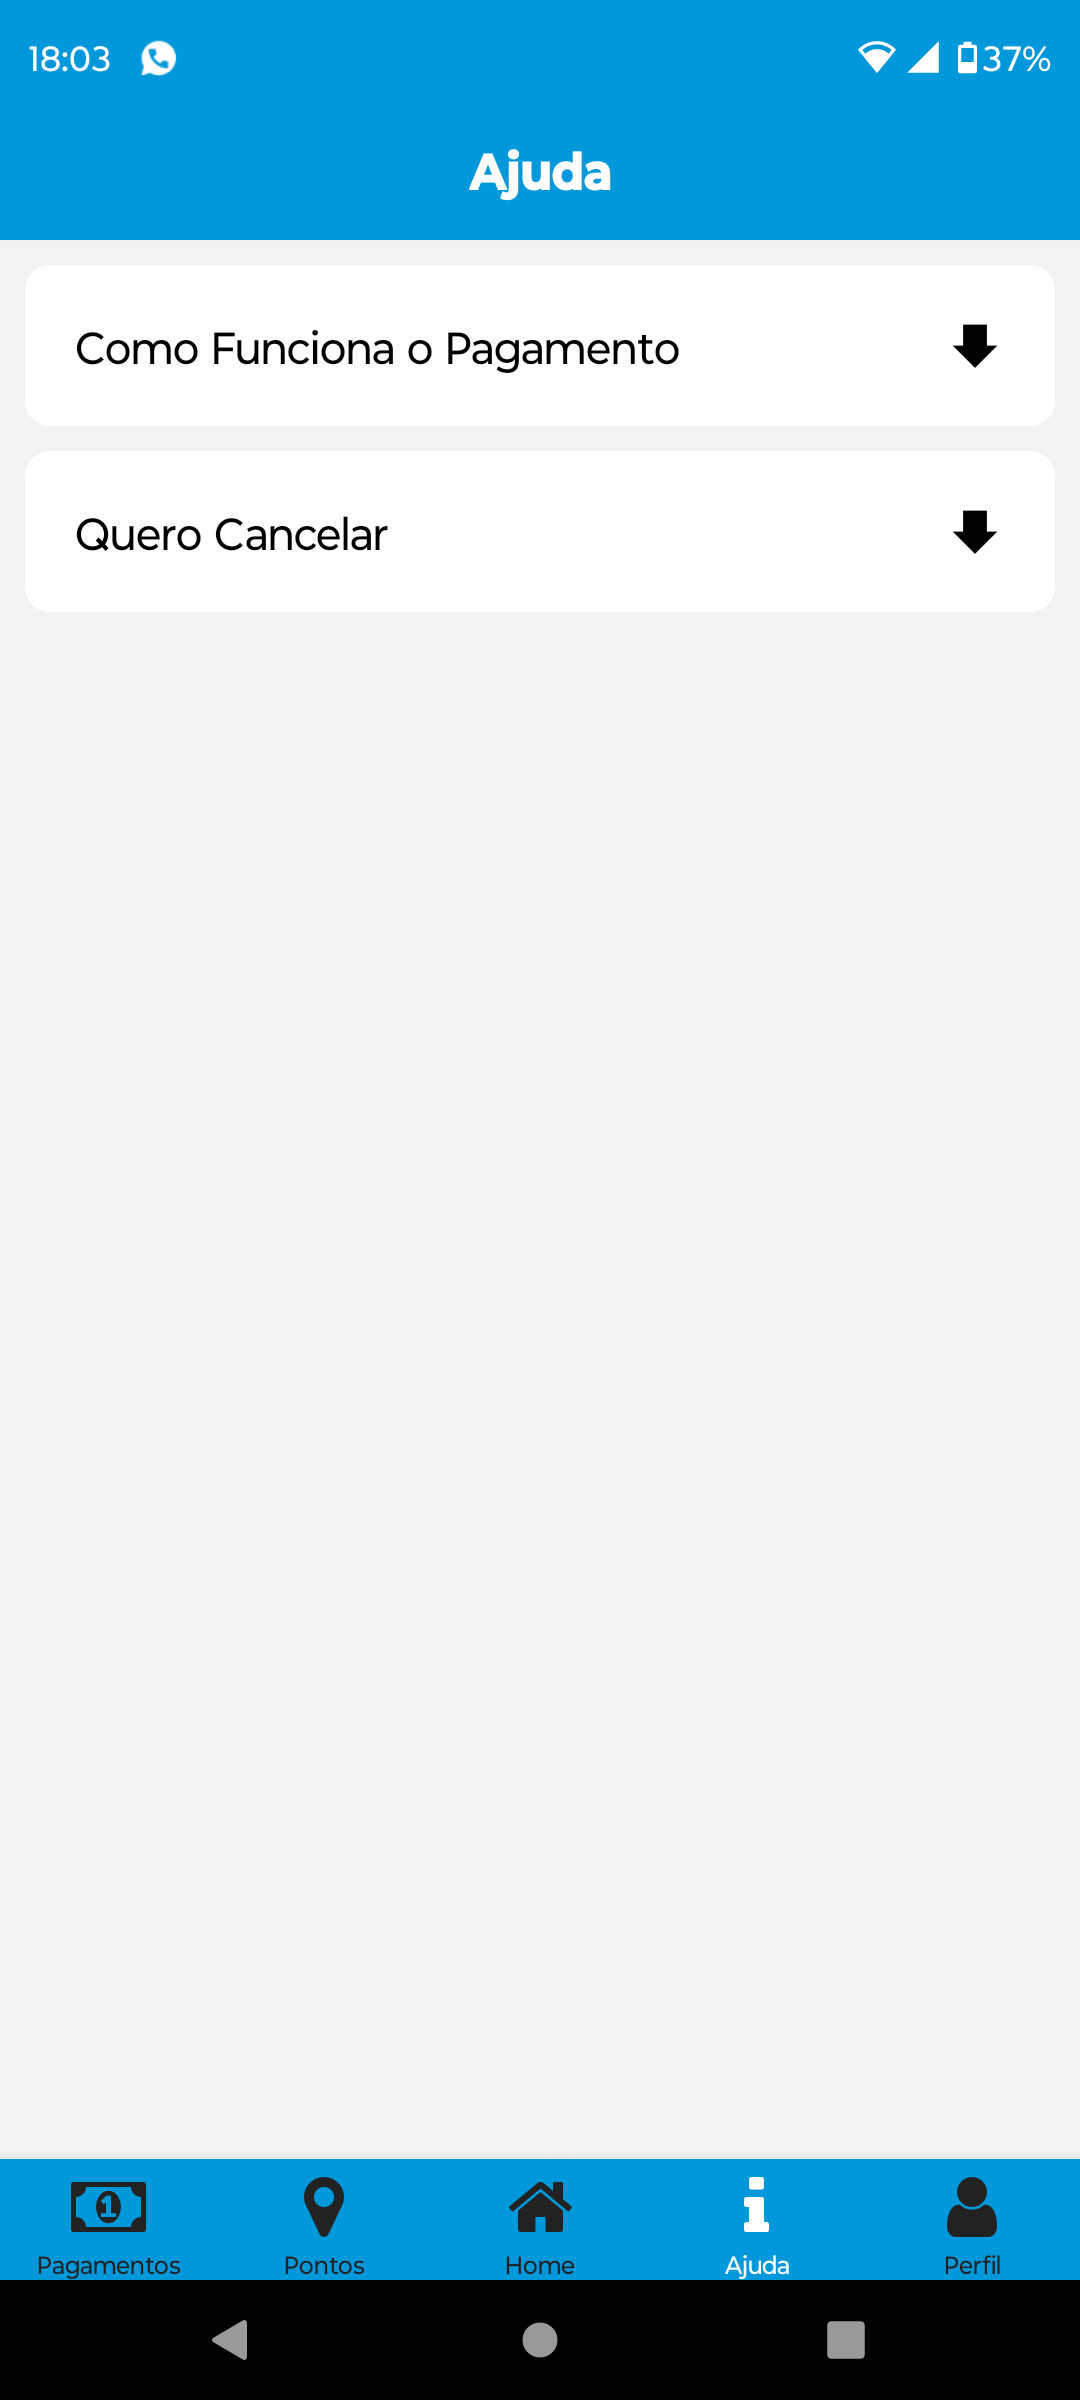
\includegraphics[width=0.8\linewidth]{Imagens/App Images User/AUAjuda1.png}
                    \caption[Imagem da Tela Ajuda do Aplicativo AESG]{ 
                    Imagem da Tela Ajuda do Aplicativo AESG}
                    \label{fig:AppTelaAjuda}
                    \legend{Fonte: O author}
                \end{minipage}%
                \begin{minipage}{0.5\textwidth}
                    \centering
                    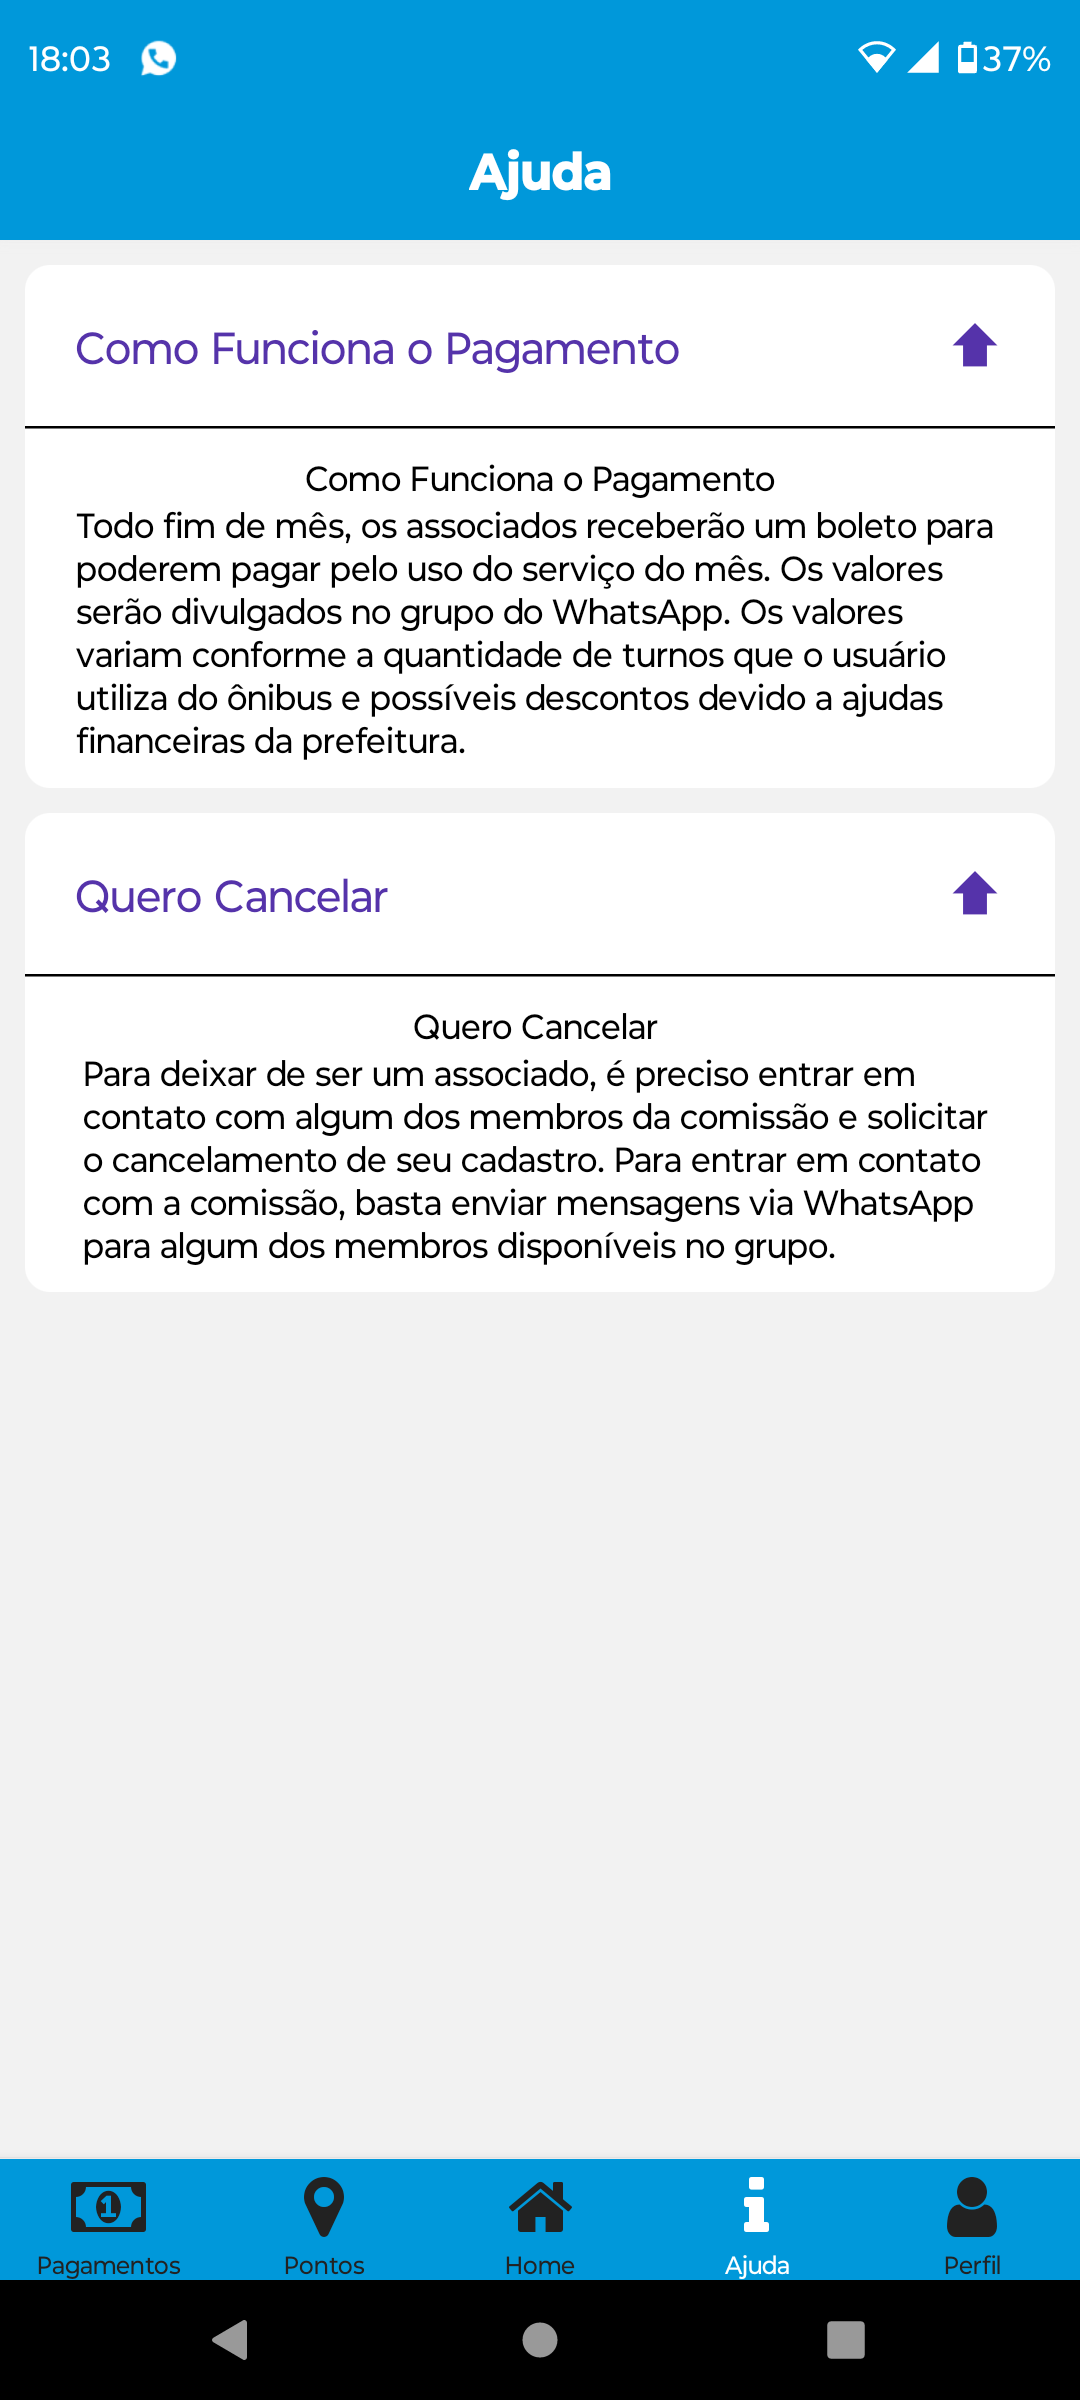
\includegraphics[width=0.8\linewidth]{Imagens/App Images User/AUAjuda2.png}
                    \caption[Imagem da Tela Ajuda do Aplicativo AESG]{ 
                    Imagem da Tela Ajuda do Aplicativo AESG}
                    \label{fig:AppTelaAjuda2}
                    \legend{Fonte: O author}
                \end{minipage}
            \end{figure}
        \subsection{Tela de Pontos}
            A partir do menu na parte inferior o usuário poderá acessar a tela de pontos, aonde ele poderá visualizar um mapa contendo demarcações dos pontos e marcação das rotas, que podem ser selecionadas pelos conjuntos de botoes seletores na parte superior da tela, e clicando em qualquer um dos pontos será possível visualizar os dados daquele ponto em específico, além de uma opção no canto inferir direto que permite definir uma rota para aquele ponto em seu aplicativo de GPS do celular, esta tela pode ser vista na Figura \ref{fig:AppTelaPontos} e Figura \ref{fig:AppTelaPontos2}.

            \begin{figure}[!h]          
                \begin{minipage}{0.5\textwidth}
                    \centering
                    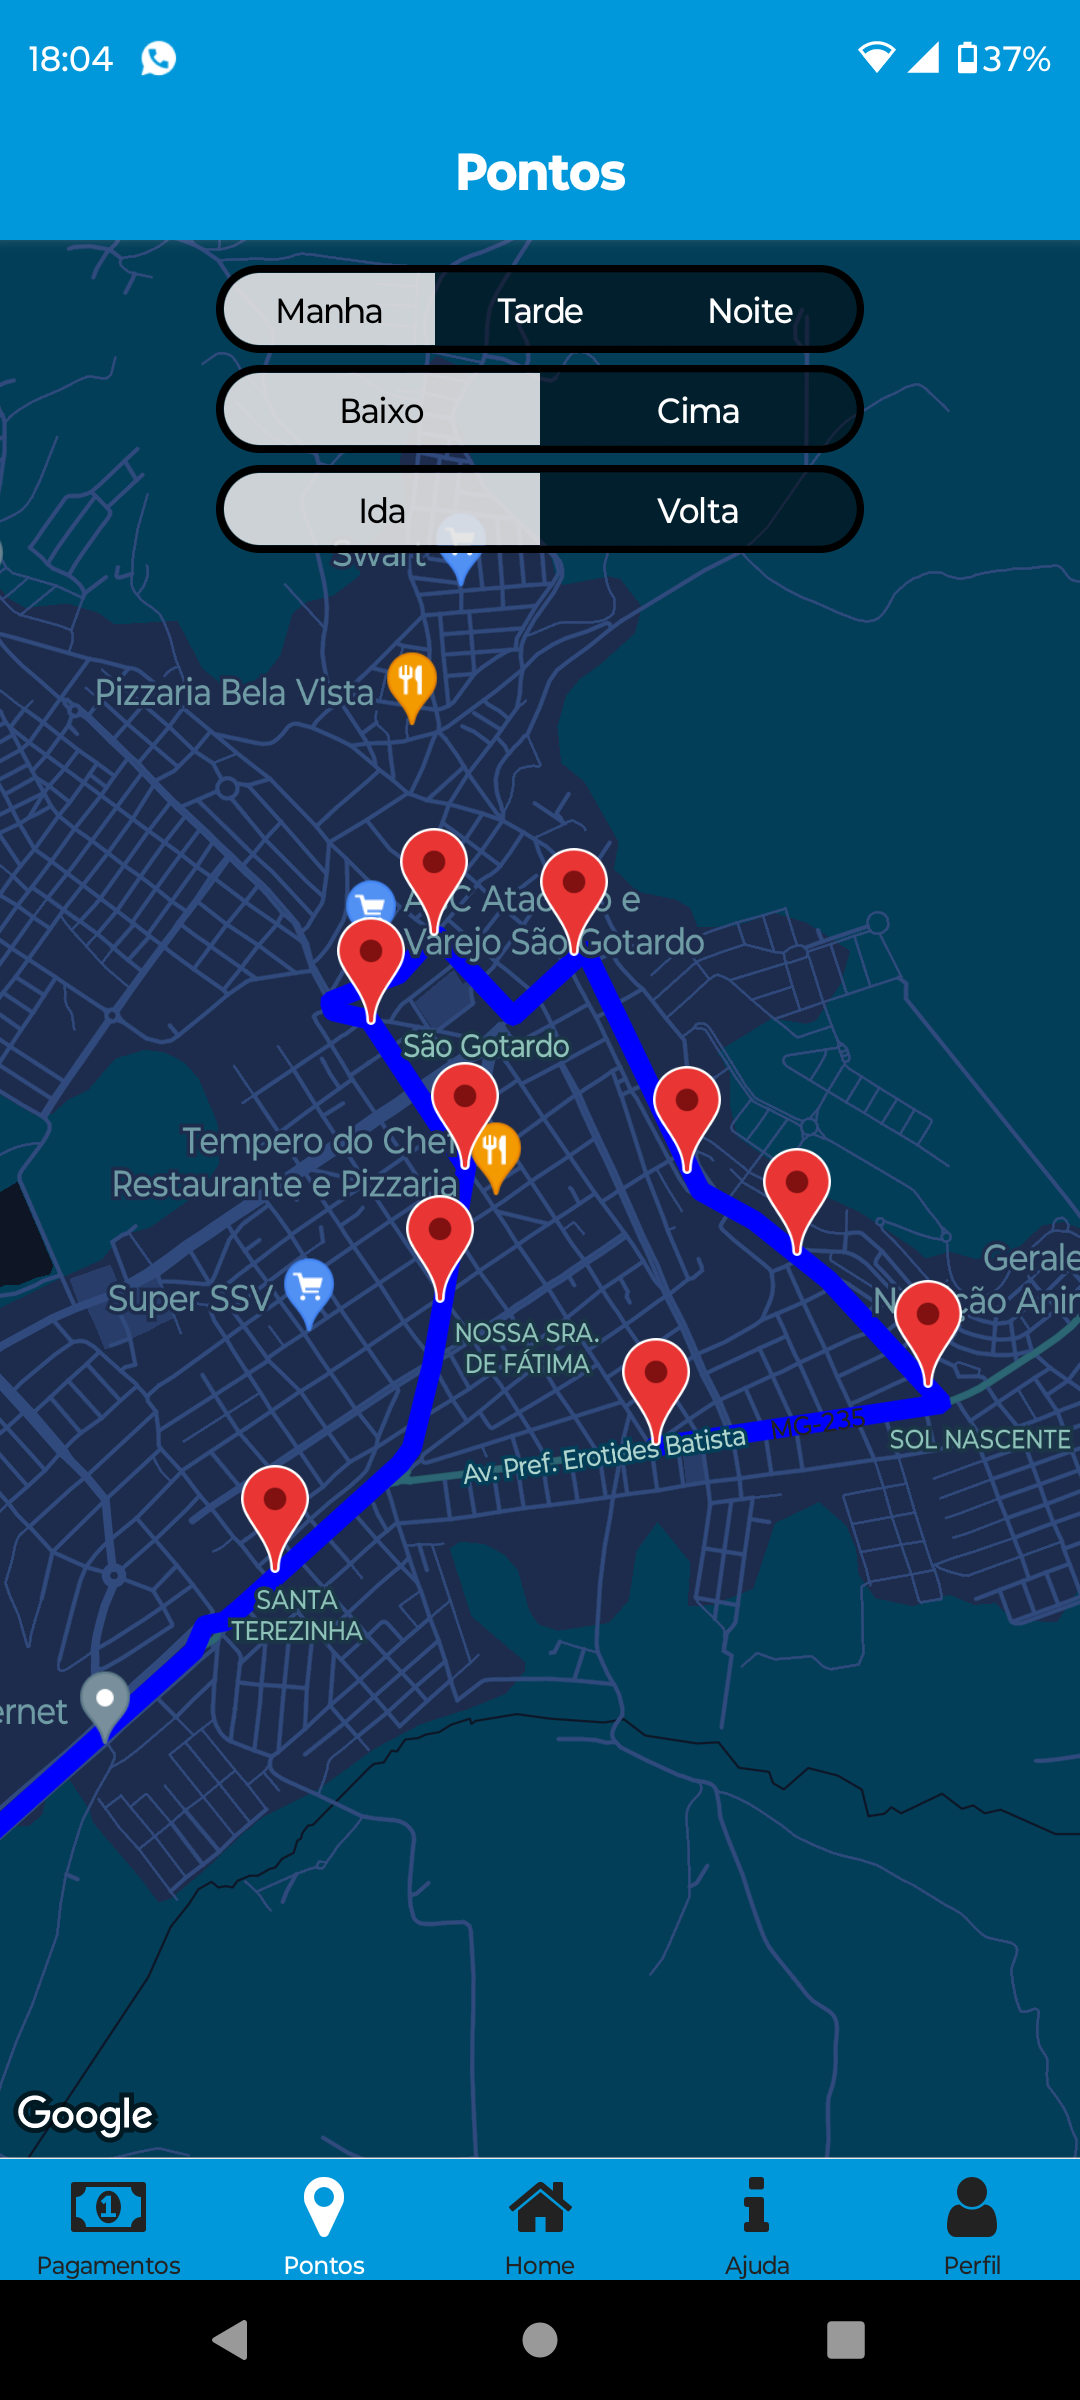
\includegraphics[width=0.8\linewidth]{Imagens/App Images User/AUPontos1.png}
                    \caption[Imagem da Tela Pontos do Aplicativo AESG]{ 
                    Imagem da Tela Pontos do Aplicativo AESG}
                    \label{fig:AppTelaPontos}
                    \legend{Fonte: O author}
                \end{minipage}%
                \begin{minipage}{0.5\textwidth}
                    \centering
                    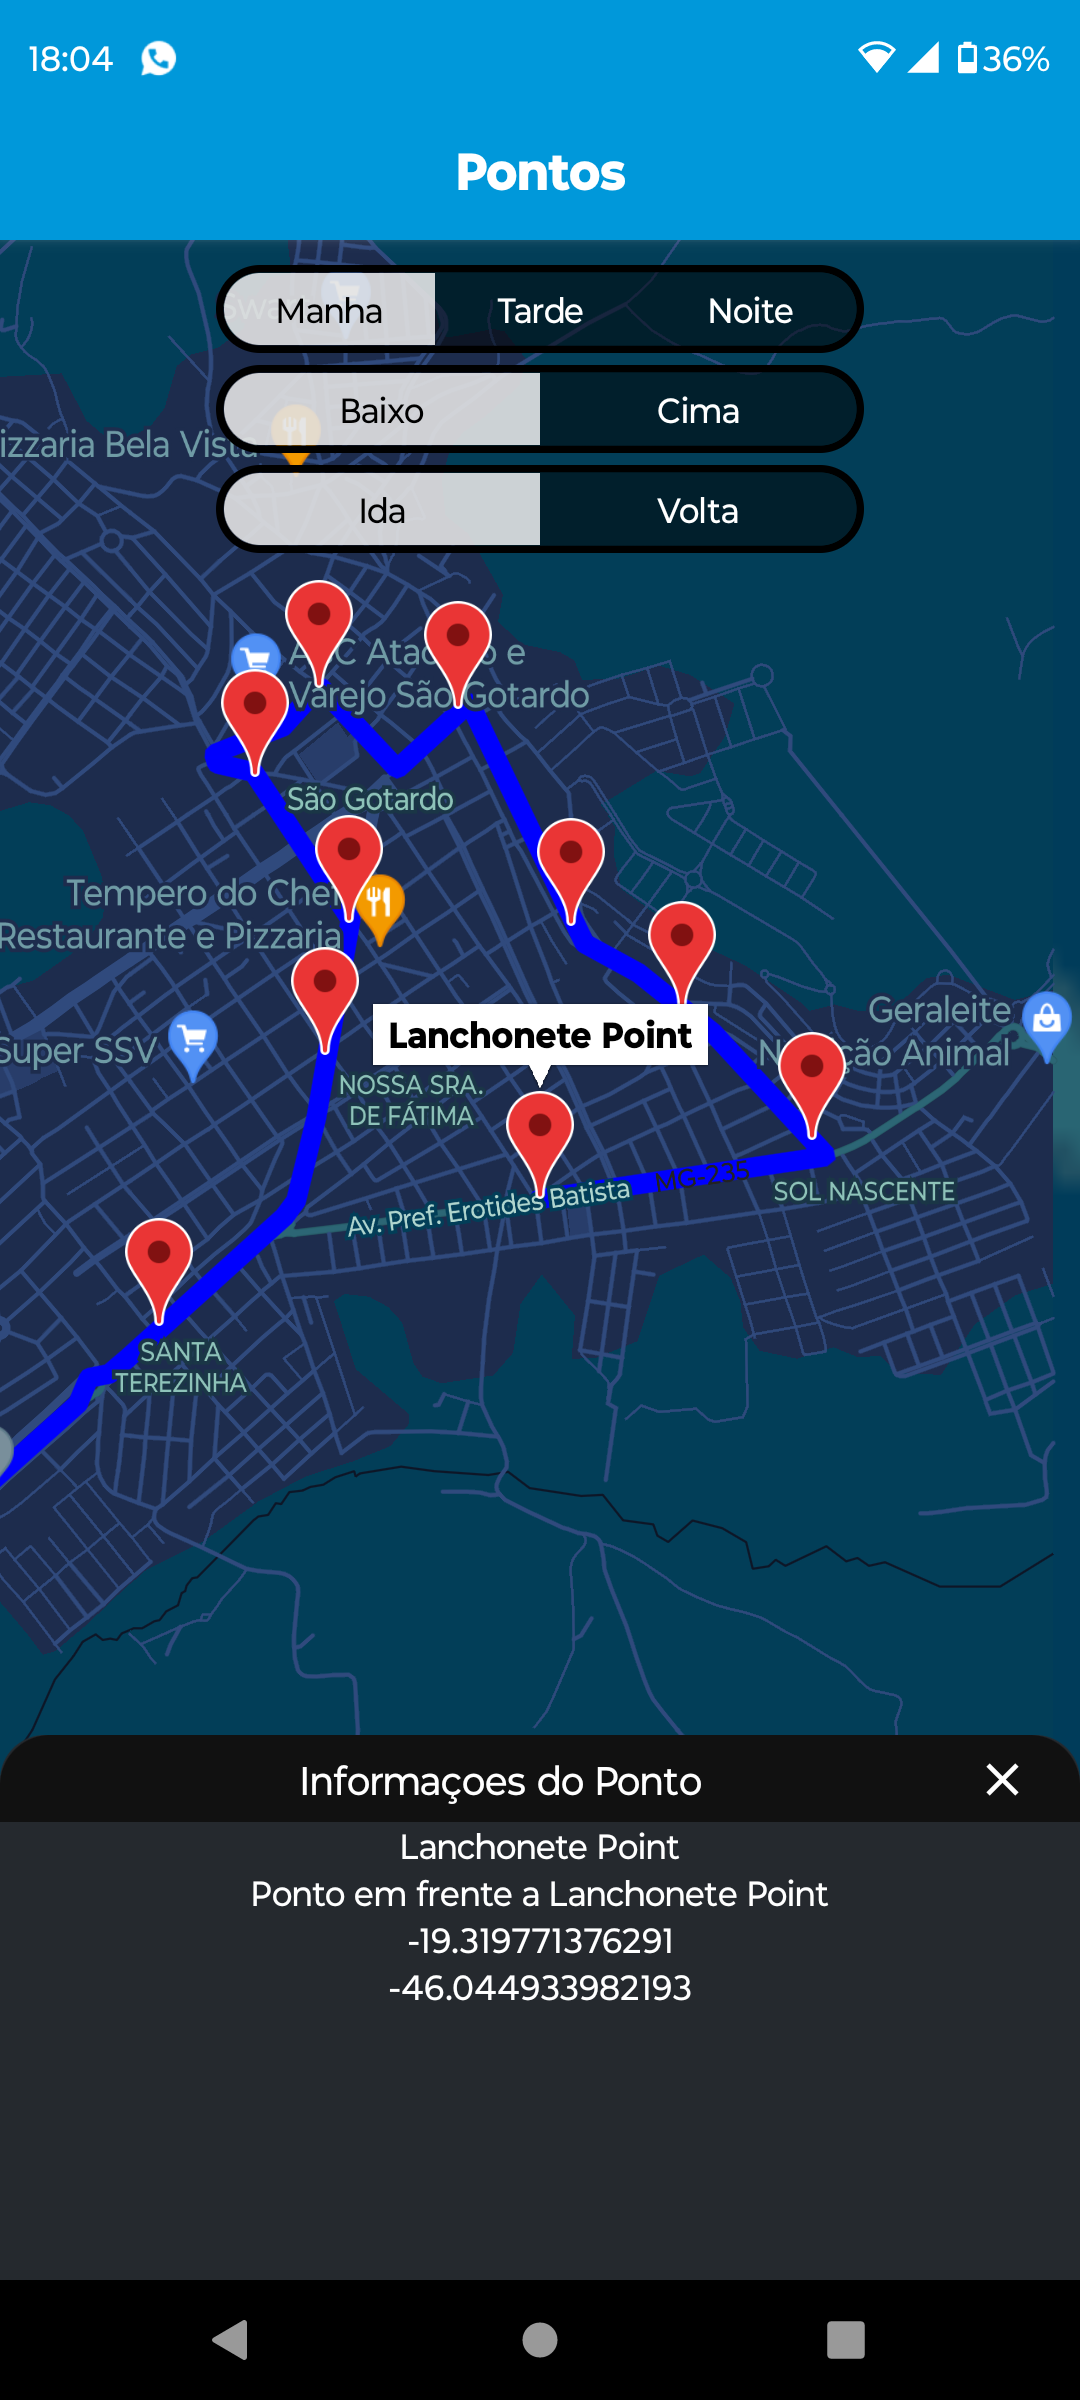
\includegraphics[width=0.8\linewidth]{Imagens/App Images User/AUPontos2.png}
                    \caption[Imagem da Tela Pontos do Aplicativo AESG]{ 
                    Imagem da Tela Pontos do Aplicativo AESG}
                    \label{fig:AppTelaPontos2}
                    \legend{Fonte: O author}
                \end{minipage}
            \end{figure}

        \subsection{Tela de Pagamentos}
            A partir do menu na parte inferior o usuário poderá acessar a tela de pagamentos, aonde ele poderá visualizar todos os pagamentos pendentes e pagos de uso do serviço, no menu da parte superior o usuário poderá selecionar os filtros dos pagamentos para visualização, serão listados os pagamentos conforme os filtros definidos e o usuário poderá clicar em qualquer um deles para ter acesso a mais dados sobre o pagamento, juntamente com os dados haverá o botão pagar aonde o usuário poderá abrir um menu para selecionar o método de pagamento desejado, tendo como opção boleto ou PIX,  esta tela pode ser vista na Figura \ref{fig:AppTelaPagamentos} e Figura \ref{fig:AppTelaPagamentos2}.

            \begin{figure}[!h]          
                \begin{minipage}{0.5\textwidth}
                    \centering
                    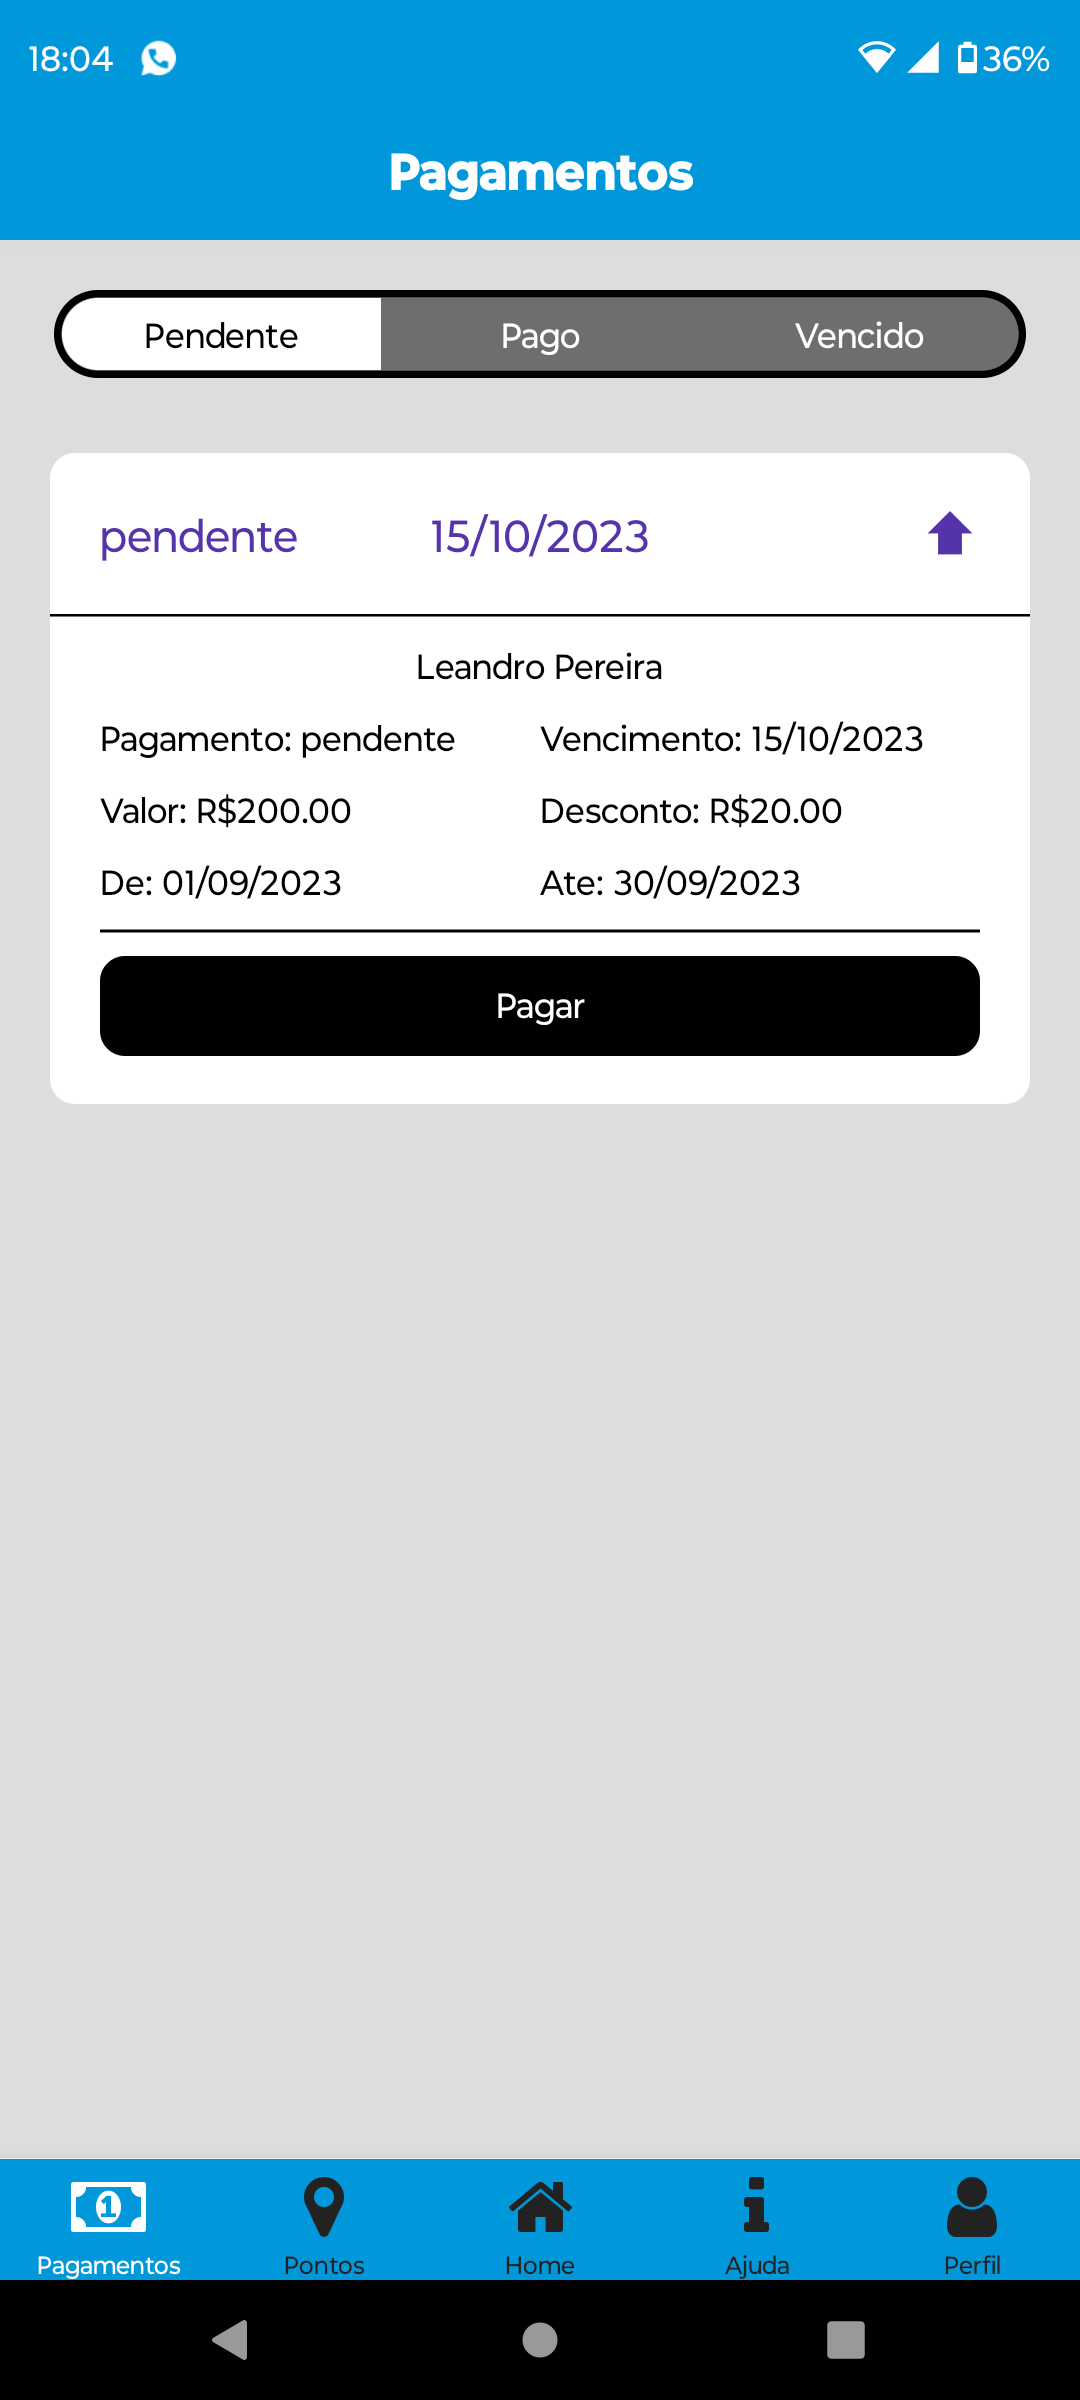
\includegraphics[width=0.8\linewidth]{Imagens/App Images User/AUPagamento1.png}
                    \caption[Imagem da Tela Pagamentos do Aplicativo AESG]{ 
                    Imagem da Tela Pagamentos do Aplicativo AESG}
                    \label{fig:AppTelaPagamentos}
                    \legend{Fonte: O author}
                \end{minipage}%
                \begin{minipage}{0.5\textwidth}
                    \centering
                    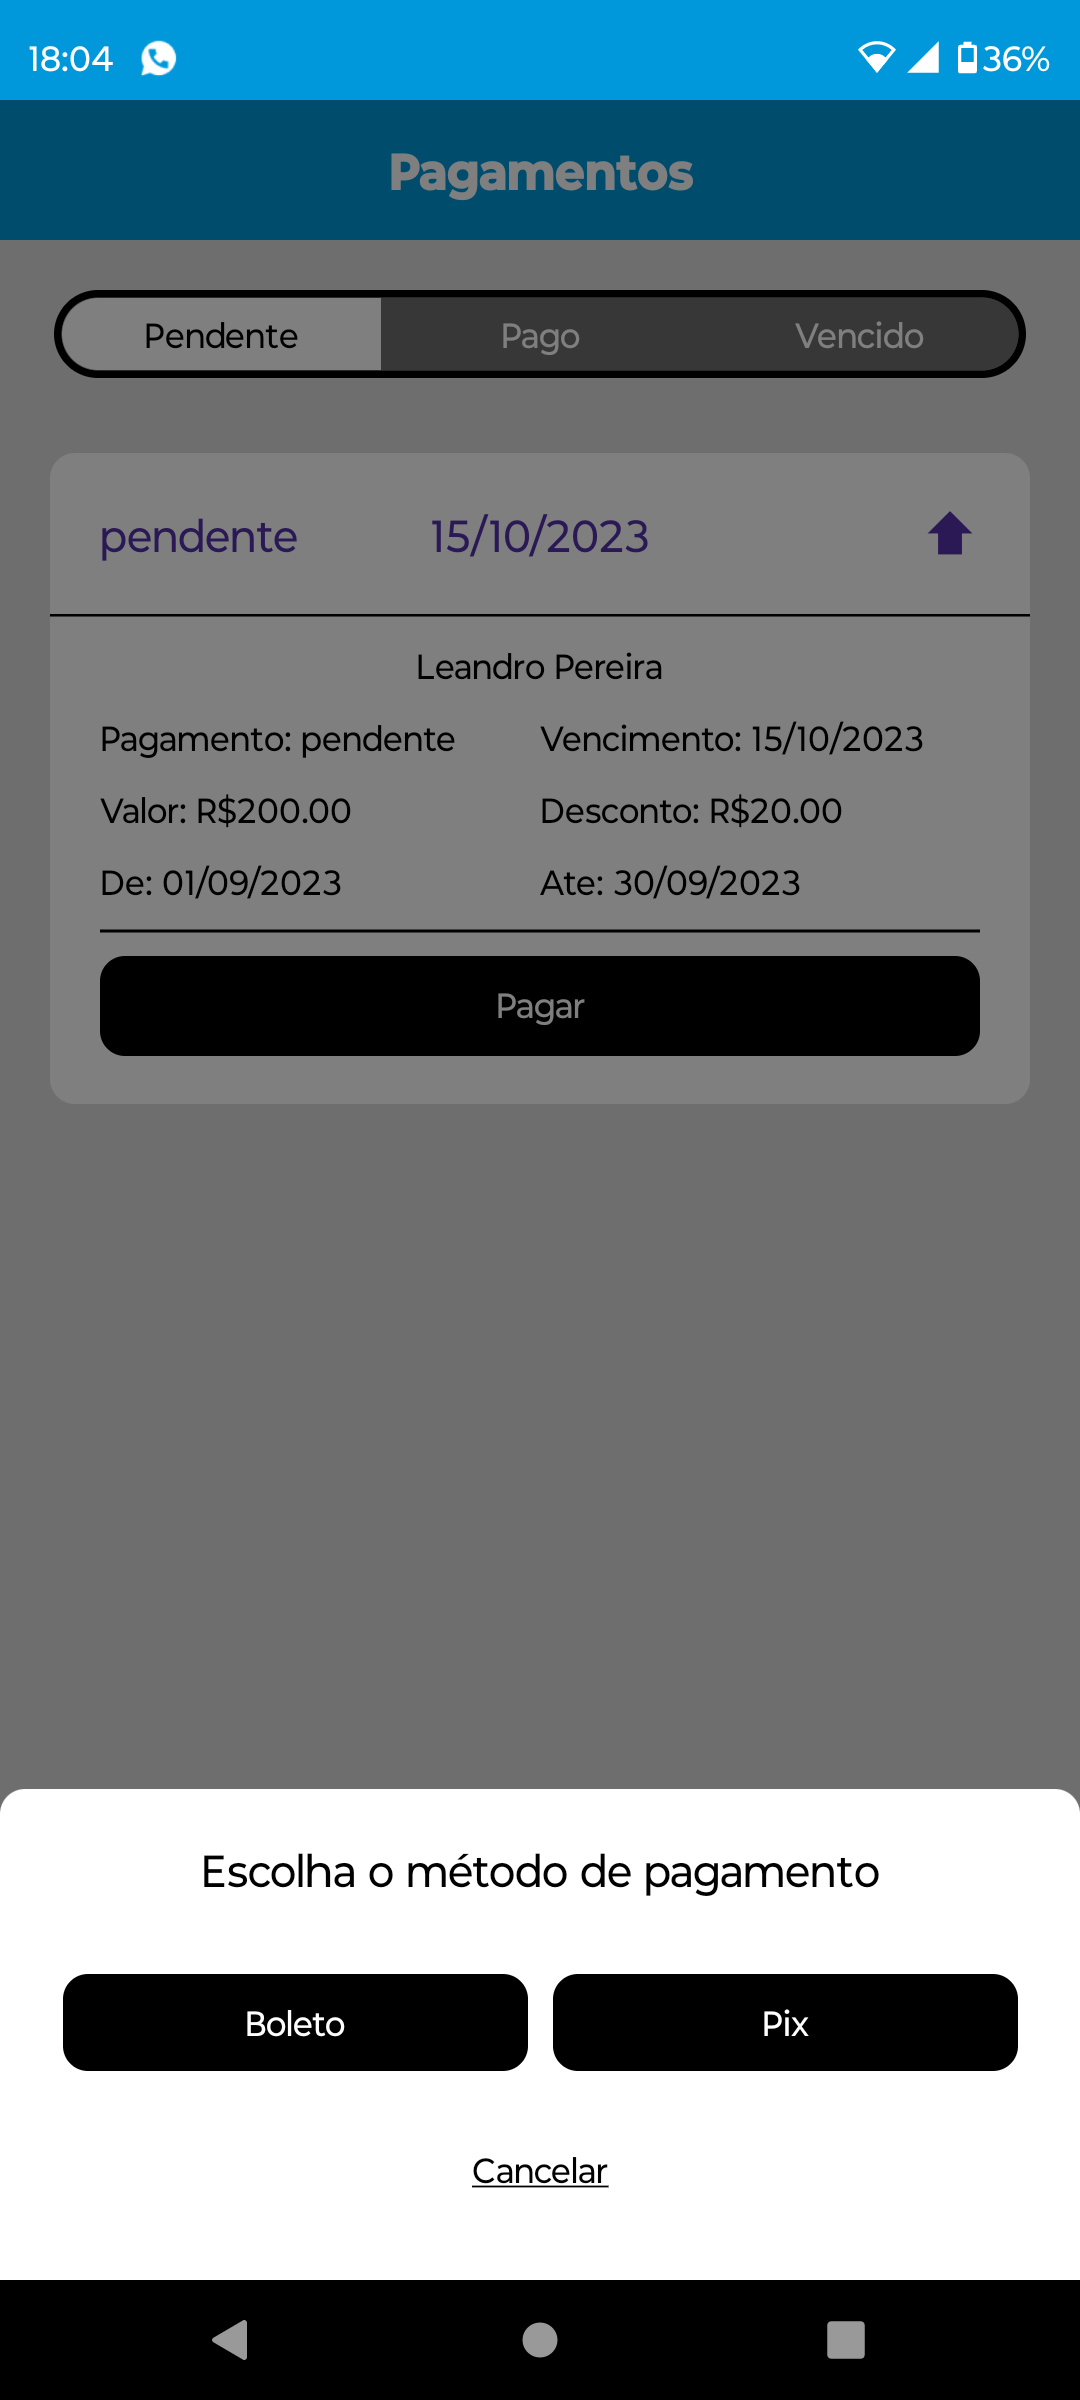
\includegraphics[width=0.8\linewidth]{Imagens/App Images User/AUPagamento2.png}
                    \caption[Imagem da Tela Pagamentos do Aplicativo AESG]{ 
                    Imagem da Tela Pagamentos do Aplicativo AESG}
                    \label{fig:AppTelaPagamentos2}
                    \legend{Fonte: O author}
                \end{minipage}
            \end{figure}
    
    %\section{Conclusões dos Resultados}
    
    
\chapter{Conclusão Geral}

\label{chap:conclusao}

Este capítulo final resume os principais resultados, contribuições e aprendizados obtidos ao longo do desenvolvimento deste trabalho. Além disso, são apresentadas sugestões para trabalhos futuros e reflexões sobre a importância do aplicativo proposto para a comunidade acadêmica.

\section{Principais Resultados}

O desenvolvimento do aplicativo de transporte universitário para as cidades de São Gotardo-MG e Rio Paranaíba-MG proporcionou resultados significativos. A implementação efetiva das funcionalidades propostas trouxe melhorias tangíveis na organização, eficiência e experiência dos usuários do transporte universitário.

O aplicativo, ao fornecer informações atualizadas sobre rotas, horários e disponibilidade de veículos, demonstrou ser uma ferramenta valiosa para otimizar o deslocamento diário dos estudantes. A integração de funcionalidades como rastreamento em tempo real e comunicação direta contribuiu para uma gestão mais eficaz do serviço.

\section{Resultados da Pesquisa de Feedback}
\label{sec:resultados-feedback}

Nesta seção, apresentamos os resultados da pesquisa de feedback realizada com os usuários do aplicativo desenvolvido para a organização do transporte universitário entre São Gotardo e a UFV-CRP. A pesquisa foi conduzida para avaliar a satisfação dos usuários com o serviço atual e obter insights sobre o desempenho e as áreas de melhoria do aplicativo.

\subsection{Perfil dos Participantes}

A pesquisa contou com a participação de vários estudantes que utilizam o serviço de transporte universitário. Entre os respondentes, foram incluídos estudantes que utilizam diferentes plataformas para acessar o serviço.

\subsection{Avaliação do Serviço Atual}

Os usuários foram questionados sobre a classificação do serviço atual oferecido pela AESG (Associação dos Estudantes de São Gotardo na UFV-CRP). As respostas foram variadas, conforme mostrado na Tabela \ref{tab:avaliacao-servico-atual}.

\begin{table}[htbp]
	\centering
	\caption{Classificação do Serviço Atual}
	\label{tab:avaliacao-servico-atual}
	\begin{tabular}{|c|c|}
		\hline
		\textbf{Classificação do Serviço} & \textbf{Frequência} \\
		\hline
		Muito Bom & 3 \\
		\hline
		Bom & 4 \\
		\hline
		Normal & 6 \\
		\hline
		Ruim & 0 \\
		\hline
		Péssimo & 0 \\
		\hline
	\end{tabular}
	\fonte{Próprio Autor}
\end{table}


\subsection{Problemas Encontrados no Serviço Atual}

Diversos problemas foram relatados pelos usuários, incluindo:
\begin{itemize}
	\item Lotação dos veículos em alguns dias, especialmente na rota noturna.
	\item Falta de educação por parte de alguns usuários.
	\item Barulho dentro dos ônibus, dificultando o descanso durante o trajeto.
\end{itemize}


\subsection{Plataforma Utilizada}

Os usuários acessam o serviço em diferentes plataformas:
\begin{itemize}
	\item Ambos (Celular e Computador): 6
	\item Celular: 5
	\item Computador: 2
\end{itemize}


\subsection{Problemas nas Plataformas}

Os participantes foram questionados sobre a existência de problemas nas plataformas utilizadas. As respostas indicaram que alguns problemas foram encontrados, mas a maioria não especificou quais plataformas apresentavam esses problemas.


\subsection{Comparação com o Sistema Atual}

Ao serem perguntados se o aplicativo foi mais fácil de usar em comparação ao sistema usado atualmente, a maioria dos respondentes que testaram o aplicativo indicou que sim.


\subsection{Vantagens e Desvantagens do Aplicativo}

Embora nem todos os participantes tenham respondido, algumas vantagens mencionadas incluem:
\begin{itemize}
	\item Facilidade de uso.
	\item Acesso rápido a informações sobre rotas e horários.
\end{itemize}


\subsection{Melhorias Sugeridas}

As melhorias sugeridas pelos usuários incluíram:
\begin{itemize}
	\item Implementação de notificações sobre mudanças de horário ou rota.
	\item Melhoria na interface para torná-la mais intuitiva.
\end{itemize}


\subsection{Opiniões Gerais sobre o Aplicativo}

Alguns participantes deixaram suas opiniões gerais sobre o aplicativo, destacando pontos positivos e áreas a serem melhoradas. Um dos respondentes mencionou que o aplicativo é uma boa iniciativa, mas ainda há espaço para aprimoramentos na usabilidade.


\section{Discussão dos Resultados}
\label{sec:discussao-resultados}

Os resultados da pesquisa de \textit{feedback} indicam que o aplicativo desenvolvido foi bem recebido pelos usuários, com várias vantagens reconhecidas em relação ao sistema atual. No entanto, alguns desafios e áreas de melhoria foram identificados, como a necessidade de aprimorar a interface e implementar funcionalidades adicionais para melhorar a experiência do usuário.


\section{Contribuições do Trabalho}

Este trabalho contribui para a área de transporte universitário ao apresentar uma solução tecnológica inovadora. A proposta de desenvolvimento de um aplicativo móvel atendeu às necessidades específicas da comunidade acadêmica, abordando desafios logísticos e financeiros enfrentados pelos estudantes no deslocamento entre São Gotardo-MG e Rio Paranaíba-MG.

Além disso, a metodologia adotada e os resultados obtidos fornecem \textit{insights} valiosos para pesquisadores e profissionais interessados no desenvolvimento de aplicativos similares em outros contextos.

\section{Conclusões e Trabalhos Futuros}
\label{sec:conclusoes-trabalhos-futuros}

Com base nos \textit{feedbacks} recebidos, é possível concluir que o aplicativo tem um grande potencial para otimizar o transporte universitário. As sugestões de melhoria fornecem uma direção clara para os próximos passos no desenvolvimento do aplicativo, visando atender ainda melhor às necessidades dos estudantes.

\subsection{Sugestões para Trabalhos Futuros}

Apesar dos avanços significativos alcançados neste trabalho, há oportunidades para futuras pesquisas e aprimoramentos. Algumas sugestões para trabalhos futuros incluem:
\begin{itemize}
	\item Realização de estudos mais aprofundados sobre a eficácia do aplicativo em longo prazo, considerando diferentes cenários e variações nas condições de uso.
	\item Implementação de funcionalidades adicionais com base no feedback contínuo dos usuários, visando sempre melhorar a experiência e a utilidade do aplicativo.
	\item Implementação de um possível rastreamento do ônibus de forma mais precisa utilizando de tecnologias como Arduino, algo parecido com o mostrado no trabalho relacionado \cite{miranda2019infraestrutura}.
	\item Exploração de parcerias com órgãos governamentais e entidades estudantis para potencializar o impacto do aplicativo e garantir seu contínuo desenvolvimento e manutenção.
	\item Uma possível expansão do aplicativo para atender ao transporte municipal de Rio Paranaíba para a UFV.
\end{itemize}

\section{Reflexões Finais}
\label{sec:reflexoes-finais}

Ao longo deste trabalho, foi possível perceber a importância de soluções inovadoras no contexto do transporte universitário. A tecnologia, quando aplicada de maneira adequada, tem o potencial de transformar positivamente a vida dos estudantes, proporcionando maior conforto, segurança e eficiência em suas jornadas acadêmicas.

A experiência de desenvolver este aplicativo não apenas contribuiu para a minha formação acadêmica, mas também reforçou a relevância de projetos que visam melhorar a acessibilidade e a qualidade de serviços essenciais, como o transporte para instituições de ensino.

\section{Considerações Finais}
\label{sec:consideracoes-finais}

Encerramos este trabalho com a satisfação de ter alcançado os objetivos propostos. O aplicativo desenvolvido representa um passo significativo na melhoria do transporte universitário entre São Gotardo-MG e Rio Paranaíba-MG.

Agradecemos a todos que contribuíram para este projeto, desde a orientação acadêmica até o apoio da comunidade acadêmica local. Esperamos que este trabalho sirva de inspiração para futuras iniciativas e que as lições aprendidas possam ser aplicadas em outros contextos.


% ----------------------------------------------------------
% ELEMENTOS PÓS-TEXTUAIS
% ----------------------------------------------------------
\postextual

% Referências bibliográficas

%\bibliography{referencias}
\linespread{1}
\printbibliography
% Caso sejam necessários apêndices ou anexos em seu documento
% Use os ambientes abaixo

%% Apêndices
%
%% Inicia os apêndices
%\begin{apendicesenv}
%
%% Imprime uma página indicando o início dos apêndices
%\partapendices
%
%\chapter{Primeiro Apêndice}
%
%\chapter{Segundo Apêndice}
%
%\end{apendicesenv}
%
%% ----------------------------------------------------------
%% Anexos
%% ----------------------------------------------------------
%\begin{anexosenv}
%
%% Imprime uma página indicando o início dos anexos
%\partanexos
%
%\chapter{Primeiro Anexo}
%\lipsum[30]
%
%\chapter{Segundo Anexo}
%\lipsum[31]
%
%\end{anexosenv}

\end{document}
